\documentclass[10pt, a4paper]{article}
\usepackage[english]{babel}
%\usepackage[brazilian]{babel}
\usepackage[utf8]{inputenc}
% \usepackage[T1]{fontenc}
\usepackage{lipsum}

% code
\usepackage{pythonhighlight}
\renewcommand{\lstlistingname}{Anexo} % Listing->Code
\usepackage{adjustbox}

% For subfigure use
\usepackage[font=small,labelfont=bf]{caption}
\usepackage{subcaption}

% Set page size and margins
% Replace `letterpaper' with`a4paper' for UK/EU standard size
\usepackage[a4paper,top=2cm,bottom=2cm,left=2cm,right=2cm,marginparwidth=2cm]{geometry}

% tabelas
\usepackage{array}
\usepackage{tabularx}
\usepackage{booktabs}

\usepackage{float}

% Useful packages
\usepackage{amsmath}
\usepackage{enumerate}

\usepackage{graphicx}
\usepackage[colorlinks=true, allcolors=blue]{hyperref}
\usepackage{cleveref}
\newcommand{\crefrangeconjunction}{--}


\begin{document}

\def\TITLE{Homework 02}
\def\DISCIPLINE{ELE 2346 - DEEP LEARNING}
\def\PROFESSOR{Raul Queiroz Feitosa}
\def\AUTHOR{Pedro Henrique Cardoso Paulo}
\def\CONTACT{pedrorjpaulo.phcp@gmail.com}
\def\DATE{May, 2023}

\title{\textbf{\TITLE} \\ \DISCIPLINE}
\author{\AUTHOR}
\date{\DATE}

\begin{titlepage}
      \begin{center}
          \vspace*{1cm}

          \Huge
          \textbf{\TITLE}

          \vspace{0.5cm}
          \LARGE
          \DISCIPLINE

          \vspace{1.5cm}

          \textbf{\AUTHOR \\ {\tt \CONTACT}}

          \vfill
          Professor: \PROFESSOR

          \vspace{0.8cm}

          
\includegraphics[width=0.2\textwidth]{../general/puc.jpg}

          \Large
          Departamento de Engenharia Mecânica\\
          PUC-RJ Pontifícia Universidade Católica do Rio de Janeiro\\
          \DATE

      \end{center}
  \end{titlepage}

\maketitle

\section{Introduction}

\subsection{Objectives}

The main objectives of this exercice is to provide the students some experience with:

\begin{itemize}
  \item The PyTorch library
  \item Segmentation models
  \item The patch strategy for dealing with big images
\end{itemize}

\subsection{Dataset}

For this exercice, the dataset will be comprised of two images that will be splitted into train, validation and test sets by creating patches of the image. Figure \ref{fig:example}
shows the images belonging to the train and test dataset.

\begin{figure}[htpb]
  \centering
  \begin{subfigure}[b]{0.32\textwidth}
      \centering
      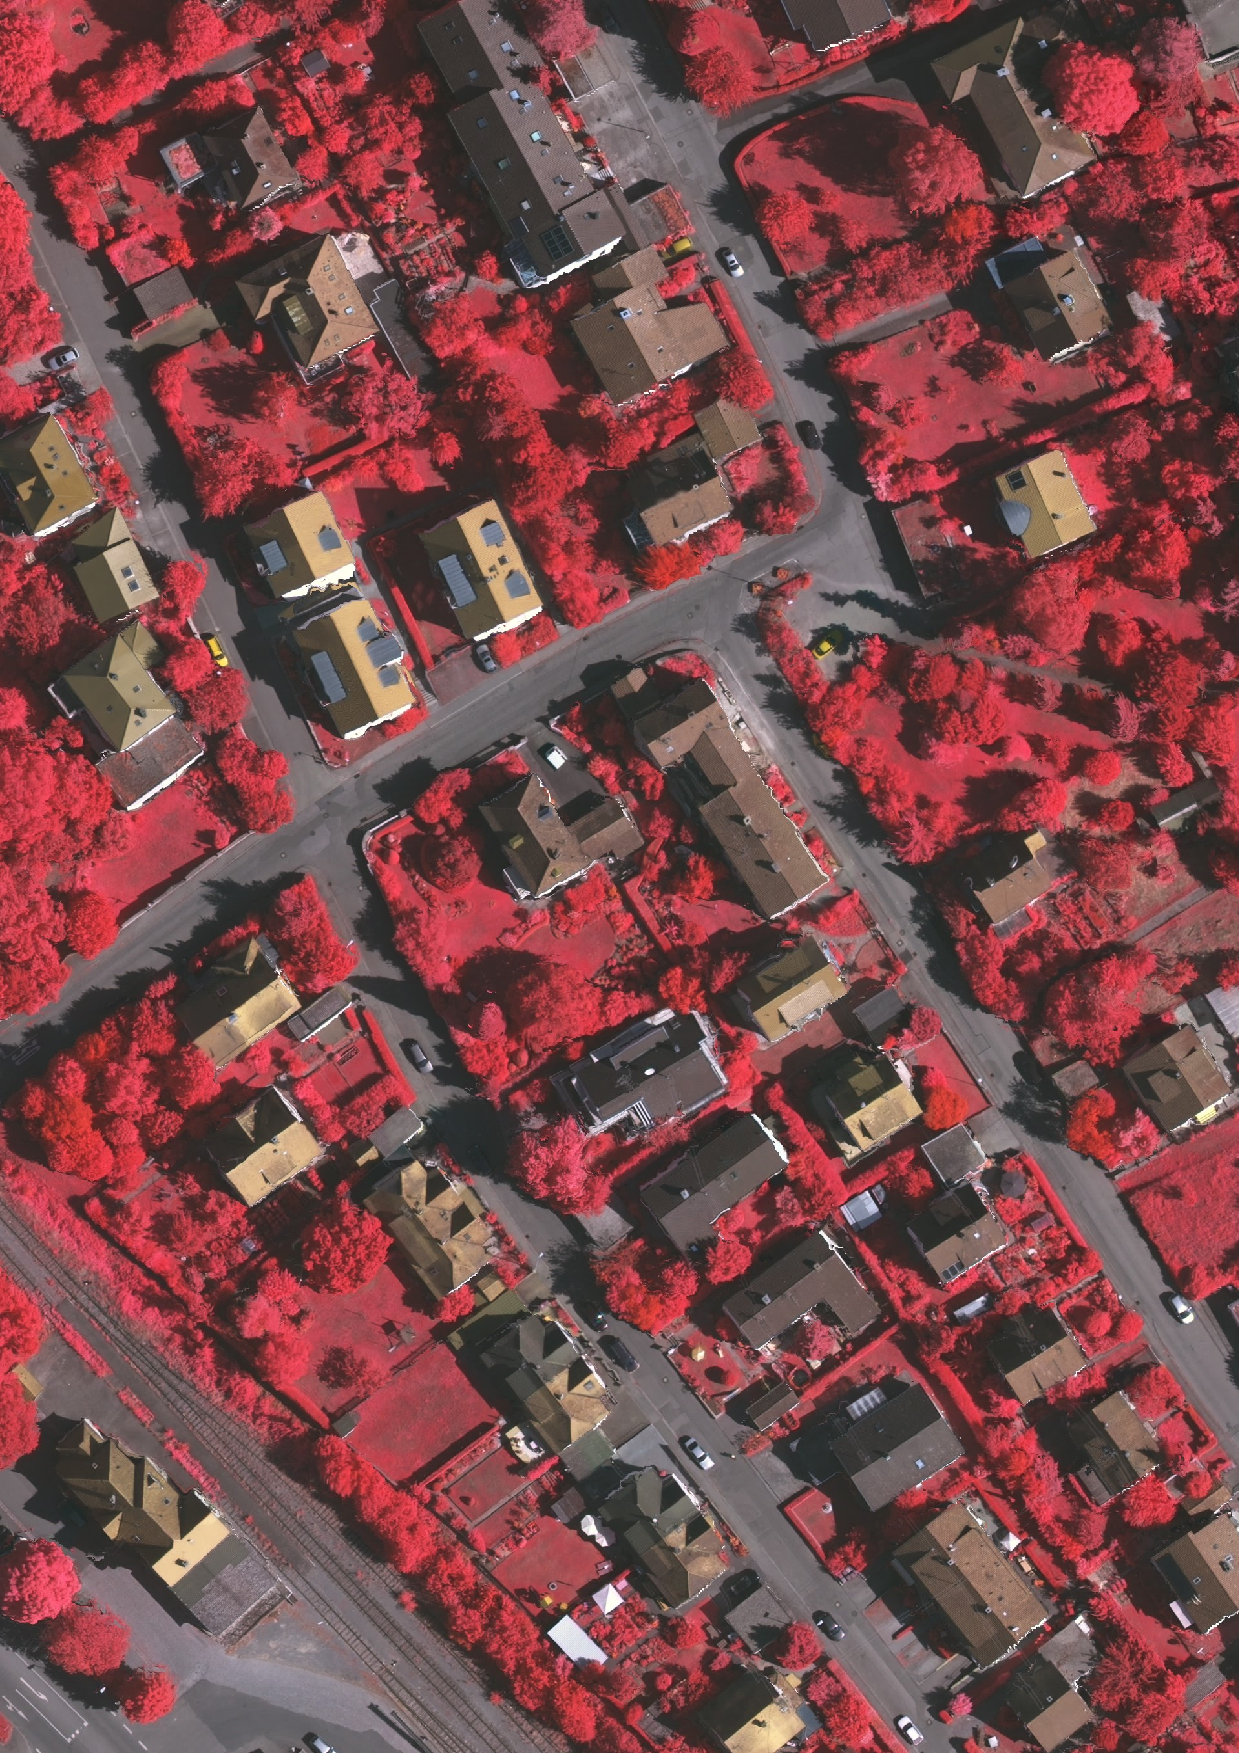
\includegraphics[width=\textwidth]{images/Image_Train.pdf}
      \caption{Train set}
      \label{fig:example_train}
  \end{subfigure}
  \hspace{0.05\textwidth}
  \begin{subfigure}[b]{0.32\textwidth}
      \centering
      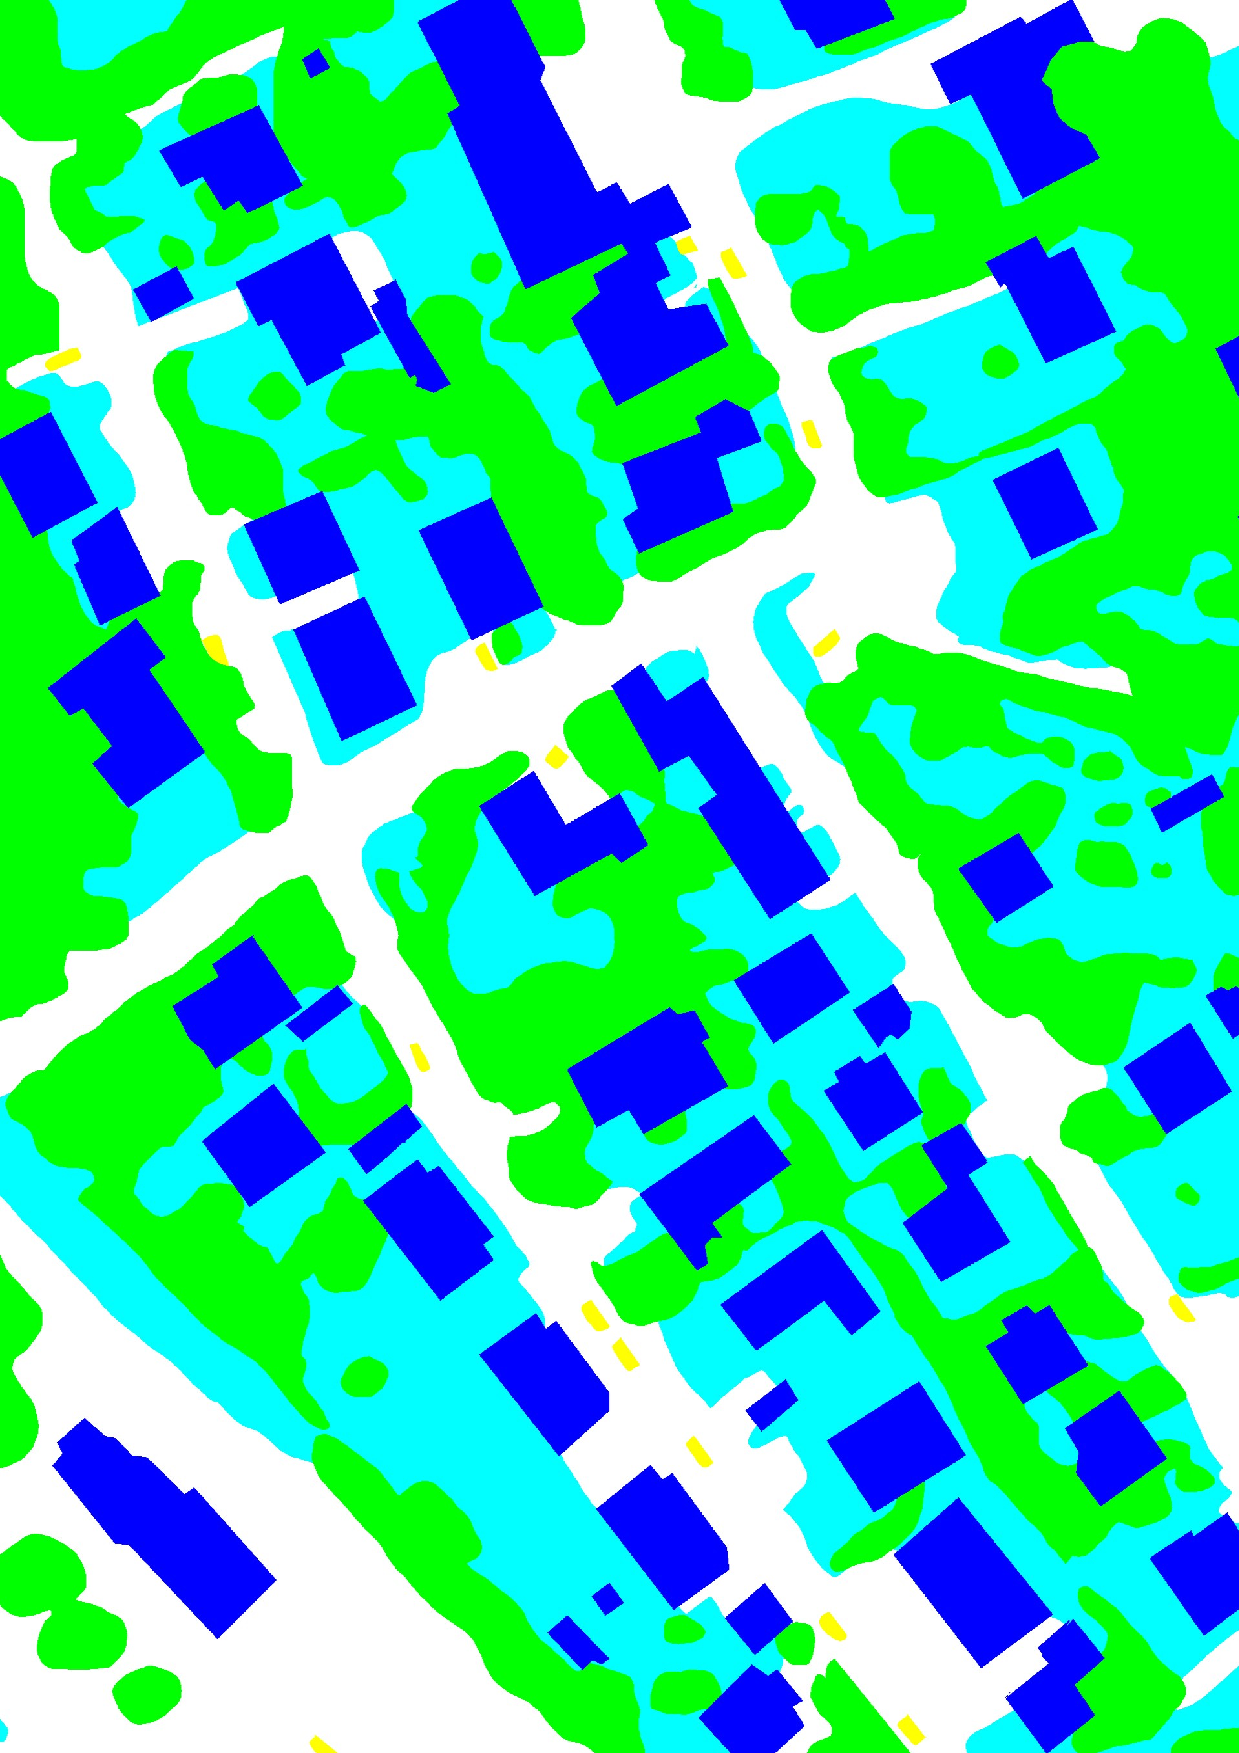
\includegraphics[width=\textwidth]{images/Reference_Train.pdf}
      \caption{Train mask}
      \label{fig:example_test}
  \end{subfigure}
  \caption{Train image to be used in the exercice}
  \label{fig:example}
\end{figure}

It is important to notice that the datasets are deeply unbalanced, with the class Car (4) having considerably less samples than the others. The table 
\ref{tab:class_distrib} summarizes the class distribution of the pixels in the train and test dataset.

\begin{table}[htpb]
  \centering
  \begin{tabular}{l|c|c|}
    Class                   &	train image	  & test image \\
    \hline
    0 (Buildings)           & 17.62\%       & 18.07\%    \\
    1 (Tree)                & 33.59\%       & 29.75\%    \\
    2 (Low vegetation)      & 25.50\%       & 35.36\%    \\
    3 (Car)                 & 00.27\%       & 00.38\%    \\
    4 (Impervious surfaces) & 23.01\%       & 16.44\%    \\
    \hline
  \end{tabular}
  \caption{Classes distribution in train and test datasets}
  \label{tab:class_distrib}
\end{table}

\subsection{Exercice}


The main objective of this notebook is to implement a DeepLabV3+ Network for semantic segmentation using Segmentation Models of PyTorch. 
The following steps should be followed:

\begin{enumerate}
  \item Split the train image for training (80\%) and validation (20\%)
  \item Generate patches from the training image (128x128, 64x64, 32x32)
  \item Train a DeepLabV3+ network using the Segmentation Models of pytorch using the ecoder \ 
        {\tt 'mobilenet\_v2'} from scratch and with pretrained weights of {\tt 'imagenet'}, {\tt encoder\_depth = 4} \
        and {\tt decoder\_channels = [256, 128, 64, 32]}\label{item:step03}
  \item For training, use the {\tt “weighted\_categorical\_crossentropy”} as a loss function. To compute the weights you must count the number of pixels of each class
  \item Evaluate the model on the test image using patches and make the mosaic to visualize the complete image
  \item Compute metrics for each class
  \item Compare and analize the results
\end{enumerate}

Use the following mean and standard deviation values according to the adopted weights initialization:

\begin{python}
  #Normalization for ImageNet
  mean_ = [0.485, 0.456, 0.406]
  std_  = [0.229, 0.224, 0.225]

  #Normalization for training from scratch
  mean_ = 0.0
  std_  = 1.0
\end{python}

\subsection{Cases of study}

From the proposed exercice, the following tests will be performed and compared regardign general error metrics and confusion matrices:

\begin{enumerate}
  \item Using imagenet weights as starting values\label{item:1}
  \begin{enumerate}[a]
    \item Creating patches of 32 x 32 pixels\label{item:1a}
    \item Creating patches of 64 x 64 pixels\label{item:1b}
    \item Creating patches of 128 x 128 pixels\label{item:1c}
  \end{enumerate}
  \item Using randomly initiated weights\label{item:2}
  \begin{enumerate}[a]
    \item Creating patches of 32 x 32 pixels\label{item:2a}
    \item Creating patches of 64 x 64 pixels\label{item:2b}
    \item Creating patches of 128 x 128 pixels\label{item:2c}
  \end{enumerate}
\end{enumerate}


\section{Methodology}

\subsection{Dataset definition}

In order to perform the tasks demanded by the exercice, the class {\tt PatchDataset} was created. This class was based on the {\tt DroneDataset} used on 
the in class exercice and has the function of reading the train image adn breaking it into patches for training the network. The python code of this class is 
exemplified below:

\begin{python}
class PatchDataset(Dataset):
    
    def __init__(self, img_path, mask_path, mean, std, transform=None, n_patches=32, stride=1):
        self.img_path = img_path
        self.mask_path = mask_path
        self.transform = transform
        self.n_patches = n_patches
        self.stride = stride
        self.mean = mean
        self.std = std

        #Reading the image
        img = cv2.imread(self.img_path)
        img = cv2.cvtColor(img, cv2.COLOR_BGR2RGB)
        mask = cv2.imread(self.mask_path, cv2.IMREAD_GRAYSCALE)
        self.img = img
        self.mask = mask
        orig_gray_lbls = np.sort(np.unique(mask))
        self.label_dict = {}
        self.classes_weights = []
        class_i = 0
        for orig_lbl in orig_gray_lbls:
          mask[mask == orig_lbl] = class_i
          self.label_dict[class_i] = orig_lbl
          print(f'Total number of elements in class {class_i}: {np.sum(mask == class_i)} ({np.sum(mask == class_i)/mask.size})')
          self.classes_weights.append(mask.size/np.sum(mask == class_i))
          class_i += 1
        
        img = torch.from_numpy(img).long()
        mask = torch.from_numpy(mask).long()

        self.img_patches = img.unfold(0,self.n_patches,self.stride).unfold(1,self.n_patches,self.stride)
        self.mask_patches = mask.unfold(0,self.n_patches,self.stride).unfold(1,self.n_patches,self.stride)
        self.img_patches_shape = self.img_patches.shape
        
    def __len__(self):
        self.img_patches_shape = self.img_patches.shape
        return self.img_patches_shape[0]*self.img_patches_shape[1]
    
    def __getitem__(self, idx):

        self.img_patches_shape = self.img_patches.shape
        
        idx_x = idx % self.img_patches_shape[0]
        idx_y = idx // self.img_patches_shape[0]

        img = self.img_patches[idx_x, idx_y, :, :, :]
        img = img.transpose(0,2).transpose(0,1).numpy().astype(np.uint8)

        mask = self.mask_patches[idx_x, idx_y, :,  :].numpy()

        if self.transform is not None:
            aug = self.transform(image=img, mask=mask)
            img = Image.fromarray(aug['image'])
            mask = aug['mask']
        
        if self.transform is None:
            img = Image.fromarray(img)
        
        t = T.Compose([T.ToTensor(), T.Normalize(self.mean, self.std)])
        img = t(img)
        mask = torch.from_numpy(mask).long()
            
        return img, mask

\end{python}

This class also estimates weights to be used by the {\tt torch.nn.CrossEntropyLoss} metric in order to train the network. The weights for each class are calculated by
the expression displayed in equation \ref{eq:weights}, where $n_i$ is the number of pixels belonging to the class $i$ in the image. It is worth noticing that this
weight corresponds to the inverse of the class distribution in the training dataset, as displayed in table \ref{tab:class_distrib}.

\begin{equation}\label{eq:weights}
  w_i = \frac{\sum{n_i}}{n_i}
\end{equation}

Another implemented class was the {\tt PatchTestDataset}, that has the objective of generating patches for executing predictions. This class is similar to the {\tt PatchDataset}
class, but also has a method that allows, given a trained model, excecute patch predictions for the input image and consolidate the results as a segmentation for the whole image area.
This method can be explored in the code below.

\begin{python}
    def predict_full(self, model, device):

      n_classes = len(self.label_dict)
      full_mask = torch.zeros((n_classes, self.img.shape[0], self.img.shape[1]))
      mean_mask = torch.zeros((n_classes, self.img.shape[0], self.img.shape[1]))
      t = T.Compose([T.ToTensor(), T.Normalize(mean, std)])
      model.eval()
      model.to(device)
      for i in range(len(self)):

        image, mask = self[i]
        idx_x = i % self.img_patches_shape[0]
        idx_y = i // self.img_patches_shape[0]

        coord_x = idx_x * self.stride
        coord_y = idx_y * self.stride

        image = t(image)
        image=image.to(device)
        mask = mask.to(device)
        with torch.no_grad():

          image = image.unsqueeze(0)
          mask = mask.unsqueeze(0)

          masked = model(image)
          masked = masked.cpu().squeeze(0)

        full_mask[:,coord_x:coord_x+self.n_patches, coord_y:coord_y+self.n_patches] += masked
        mean_mask[:,coord_x:coord_x+self.n_patches, coord_y:coord_y+self.n_patches] = torch.ones(masked.shape)
  
      img = torch.from_numpy(self.img).long()
      img = img.numpy().astype(np.uint8)

      img = Image.fromarray(img)
      real_mask = torch.from_numpy(self.mask).long()
      full_mask /= mean_mask
      pred_mask = full_mask.argmax(dim=0)

      return img, real_mask, pred_mask
\end{python}

It is worth mentioning that, since different patches can have intersections, the convention used for these cases is to consider the result for the intersection as
the simple average of all the patches that cover that area.

\subsection{Train and validation split}

In order to perform validation, the dataset created by dividing the train image in patches as splitted using the torch functionality {\tt SubsetRandomSampler}. After
that, two {\tt DataLoaders} were created for train and validation. The code for this particular step is presented below.

\begin{python}
# Creating data indices for training and validation splits:
dataset_size = len(dataset)
indices = list(range(dataset_size))
split = int(np.floor(validation_split * dataset_size))
if shuffle_dataset :
    np.random.seed(random_seed)
    np.random.shuffle(indices)
train_indices, val_indices = indices[split:], indices[:split]

# Creating PT data samplers and loaders:
train_sampler = SubsetRandomSampler(train_indices)
valid_sampler = SubsetRandomSampler(val_indices)

train_loader = torch.utils.data.DataLoader(dataset, batch_size=batch_size, 
                                           sampler=train_sampler)
validation_loader = torch.utils.data.DataLoader(dataset, batch_size=batch_size,
                                                sampler=valid_sampler)
\end{python}

\subsection{Hyperparameter selection}

In this exercice, the only hyperparameters that allowed some tunning where the stride of the patches, the parameters related to the optimization epochs and the 
maximum number of epochs. The selected stride was 16 in order to allow at least 50\% overlapping in the 32 x 32 filter case. Also, the number of epochs was raised
to 20 based on some preliminary runs made with the network, that showed in the history plots that there was still some room for improvement of the model by allowing
more training epochs. The parameters regarding the optimization process (learning rate, optimizer) were kept unchanged.

Other relevant comment regarding hyperparameters is that, due to limitations regarding the {\tt segmentation\-models-pytorch} package API, the proposed hyperparameters
to be used in the DeepLabV3+ model and listed in the step \ref{item:step03} of the exercice were not possible. In order to comply with the limitations of the API,
the following configuration were used:

\begin{python}
model = smp.DeepLabV3Plus('mobilenet_v2', encoder_weights='imagenet', classes=5, decoder_channels=256)
\end{python}

It is worth mentioning that, while the limitation of the {\tt decoder\_channels} is documented on the package's documentation, the limitatin on the {\tt classes} 
parameter seems to be an implementation error and only the default value $5$ worked on this case. For more information regarding the DeepLabV3+ model API, refer
to the package \href{https://smp.readthedocs.io/en/latest/models.html#id9}{documentation}.

\newpage
\section{Results and discussions}

\subsection{Colab Notebook}

All the code, examples and tests made are documented on the following Colab Notebooks. 

\begin{itemize}
  \item \href{https://colab.research.google.com/drive/1CsJtybd_mc1ewyKjQQcVnqqpMvM5mJwv?usp=sharing}{Link to the Colab Notebook}
  \item \href{https://colab.research.google.com/drive/1BkBRiBi91MBf_vex8Zw54tjMMbIPAN75?usp=sharing}{Link to the Colab Notebook used for metrics calculation}
\end{itemize}
\subsection{Item \ref{item:1a}}

Figure \ref{fig:q1a_metrics} shows the convergency of the 20 epochs using the ImageNet weights as initialization and dividing the train image into 32 x 32 patches 
with a stride of 16 pixels. It is possible to see that the value of 20 epochs seems to be a reasonable value for the problem with no overfitting (train and validation
with very different performances) and apparently a final value very close to the minimum achievable with more epochs. More epochs could perhaps improve the final result,
but given the computational cost for the problem, the result obtained for this case is considered satisfactory.

\begin{figure}[htpb]
  \centering
  \begin{subfigure}[b]{0.32\textwidth}
      \centering
      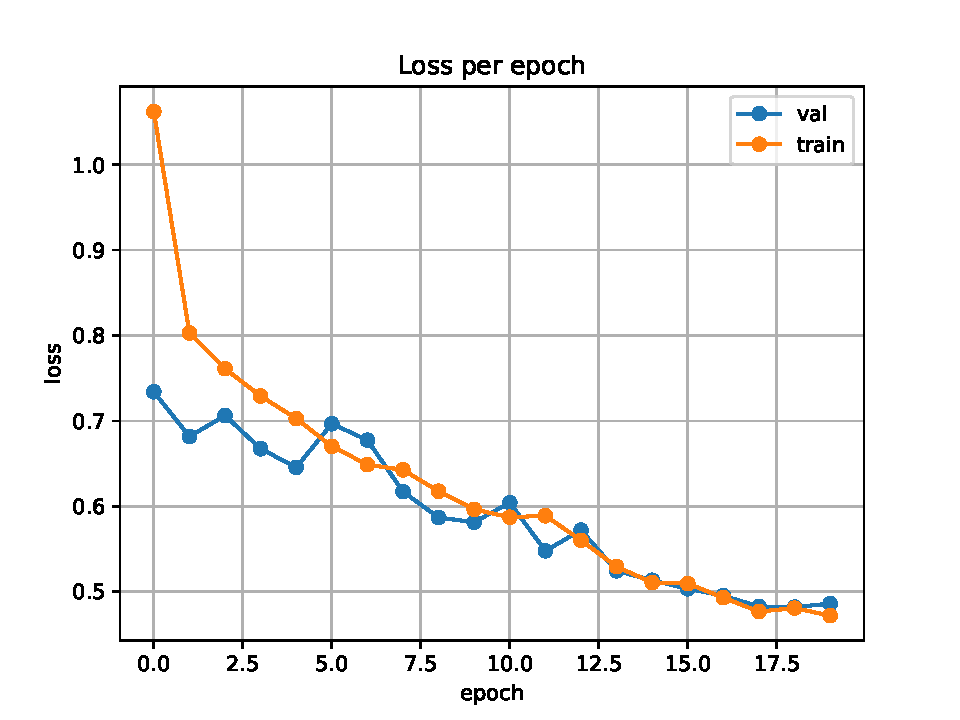
\includegraphics[width=\textwidth]{images/Patch32_imagenet_loss.pdf}
      \caption{Loss evolution}
      \label{fig:q1a_loss}
  \end{subfigure}
  \hfill
  \begin{subfigure}[b]{0.32\textwidth}
    \centering
    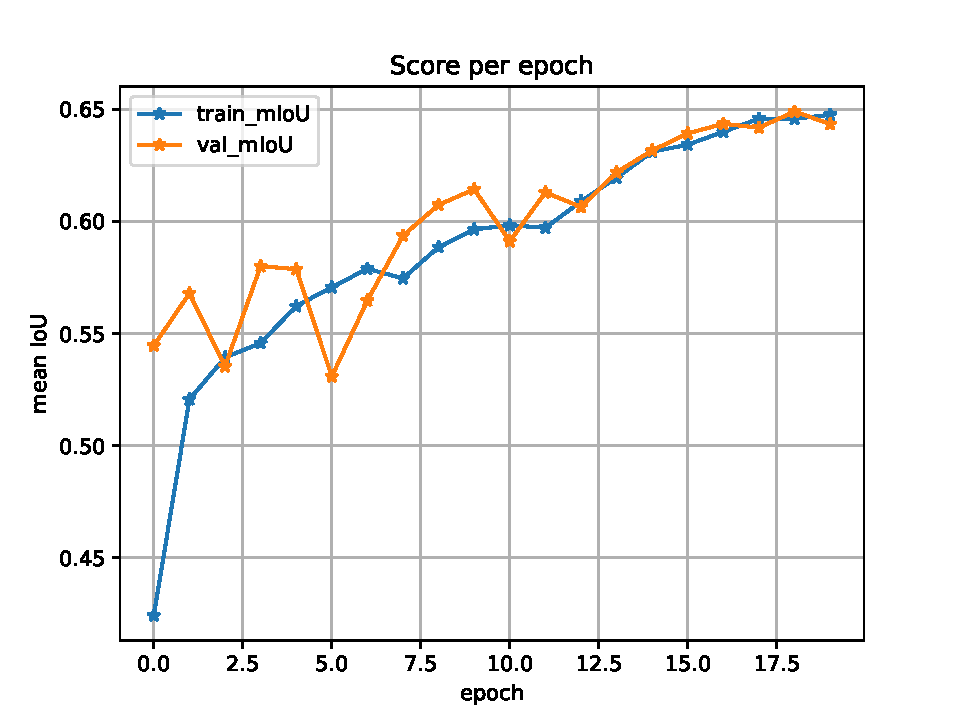
\includegraphics[width=\textwidth]{images/Patch32_imagenet_score.pdf}
    \caption{Score evolution}
    \label{fig:q1a_score}
  \end{subfigure}
  \hfill
  \begin{subfigure}[b]{0.32\textwidth}
      \centering
      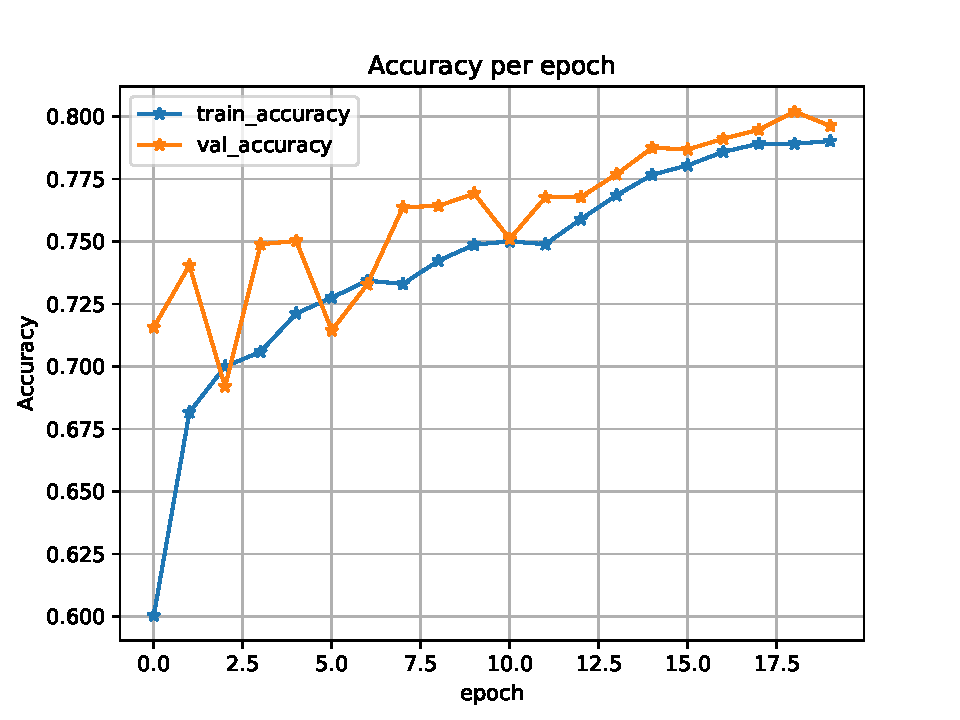
\includegraphics[width=\textwidth]{images/Patch32_imagenet_acc.pdf}
      \caption{Accuracy evolution}
      \label{fig:q1a_acc}
  \end{subfigure}
  \caption{Metrics evolution during training for item \ref{item:1a}}
  \label{fig:q1a_metrics}
\end{figure}

In figure \ref{fig:q1a_results} we see a comparison of the results obtained by running a prediction in the train and test datasets. The error metric indicated
in the image is the mean IoU between the classes. For this first test it is worth noticing that good results were obtained for both the train and test results,
but there is still room for improvement. The model seems to present great confusion between the classes 1 (Tree) and 2 (Low vegetation), which is justifiable
for their similarities regarding color and aspect when seen from above. It is also worth mentioning that the class 3 (Car) i considerably well predicted considering
that it is a subsampled class, ti all thanks to the weights selected. Also worth mentioning is that the improvement in the class 3 prediction also comes with a cost,
since it is possible to see in the results that two near class 3 regions tend to be merged, supressing class 4 (Impervious surfaces) between them.

\begin{figure}[htpb]
  \centering
  \begin{subfigure}[b]{0.45\textwidth}
      \centering
      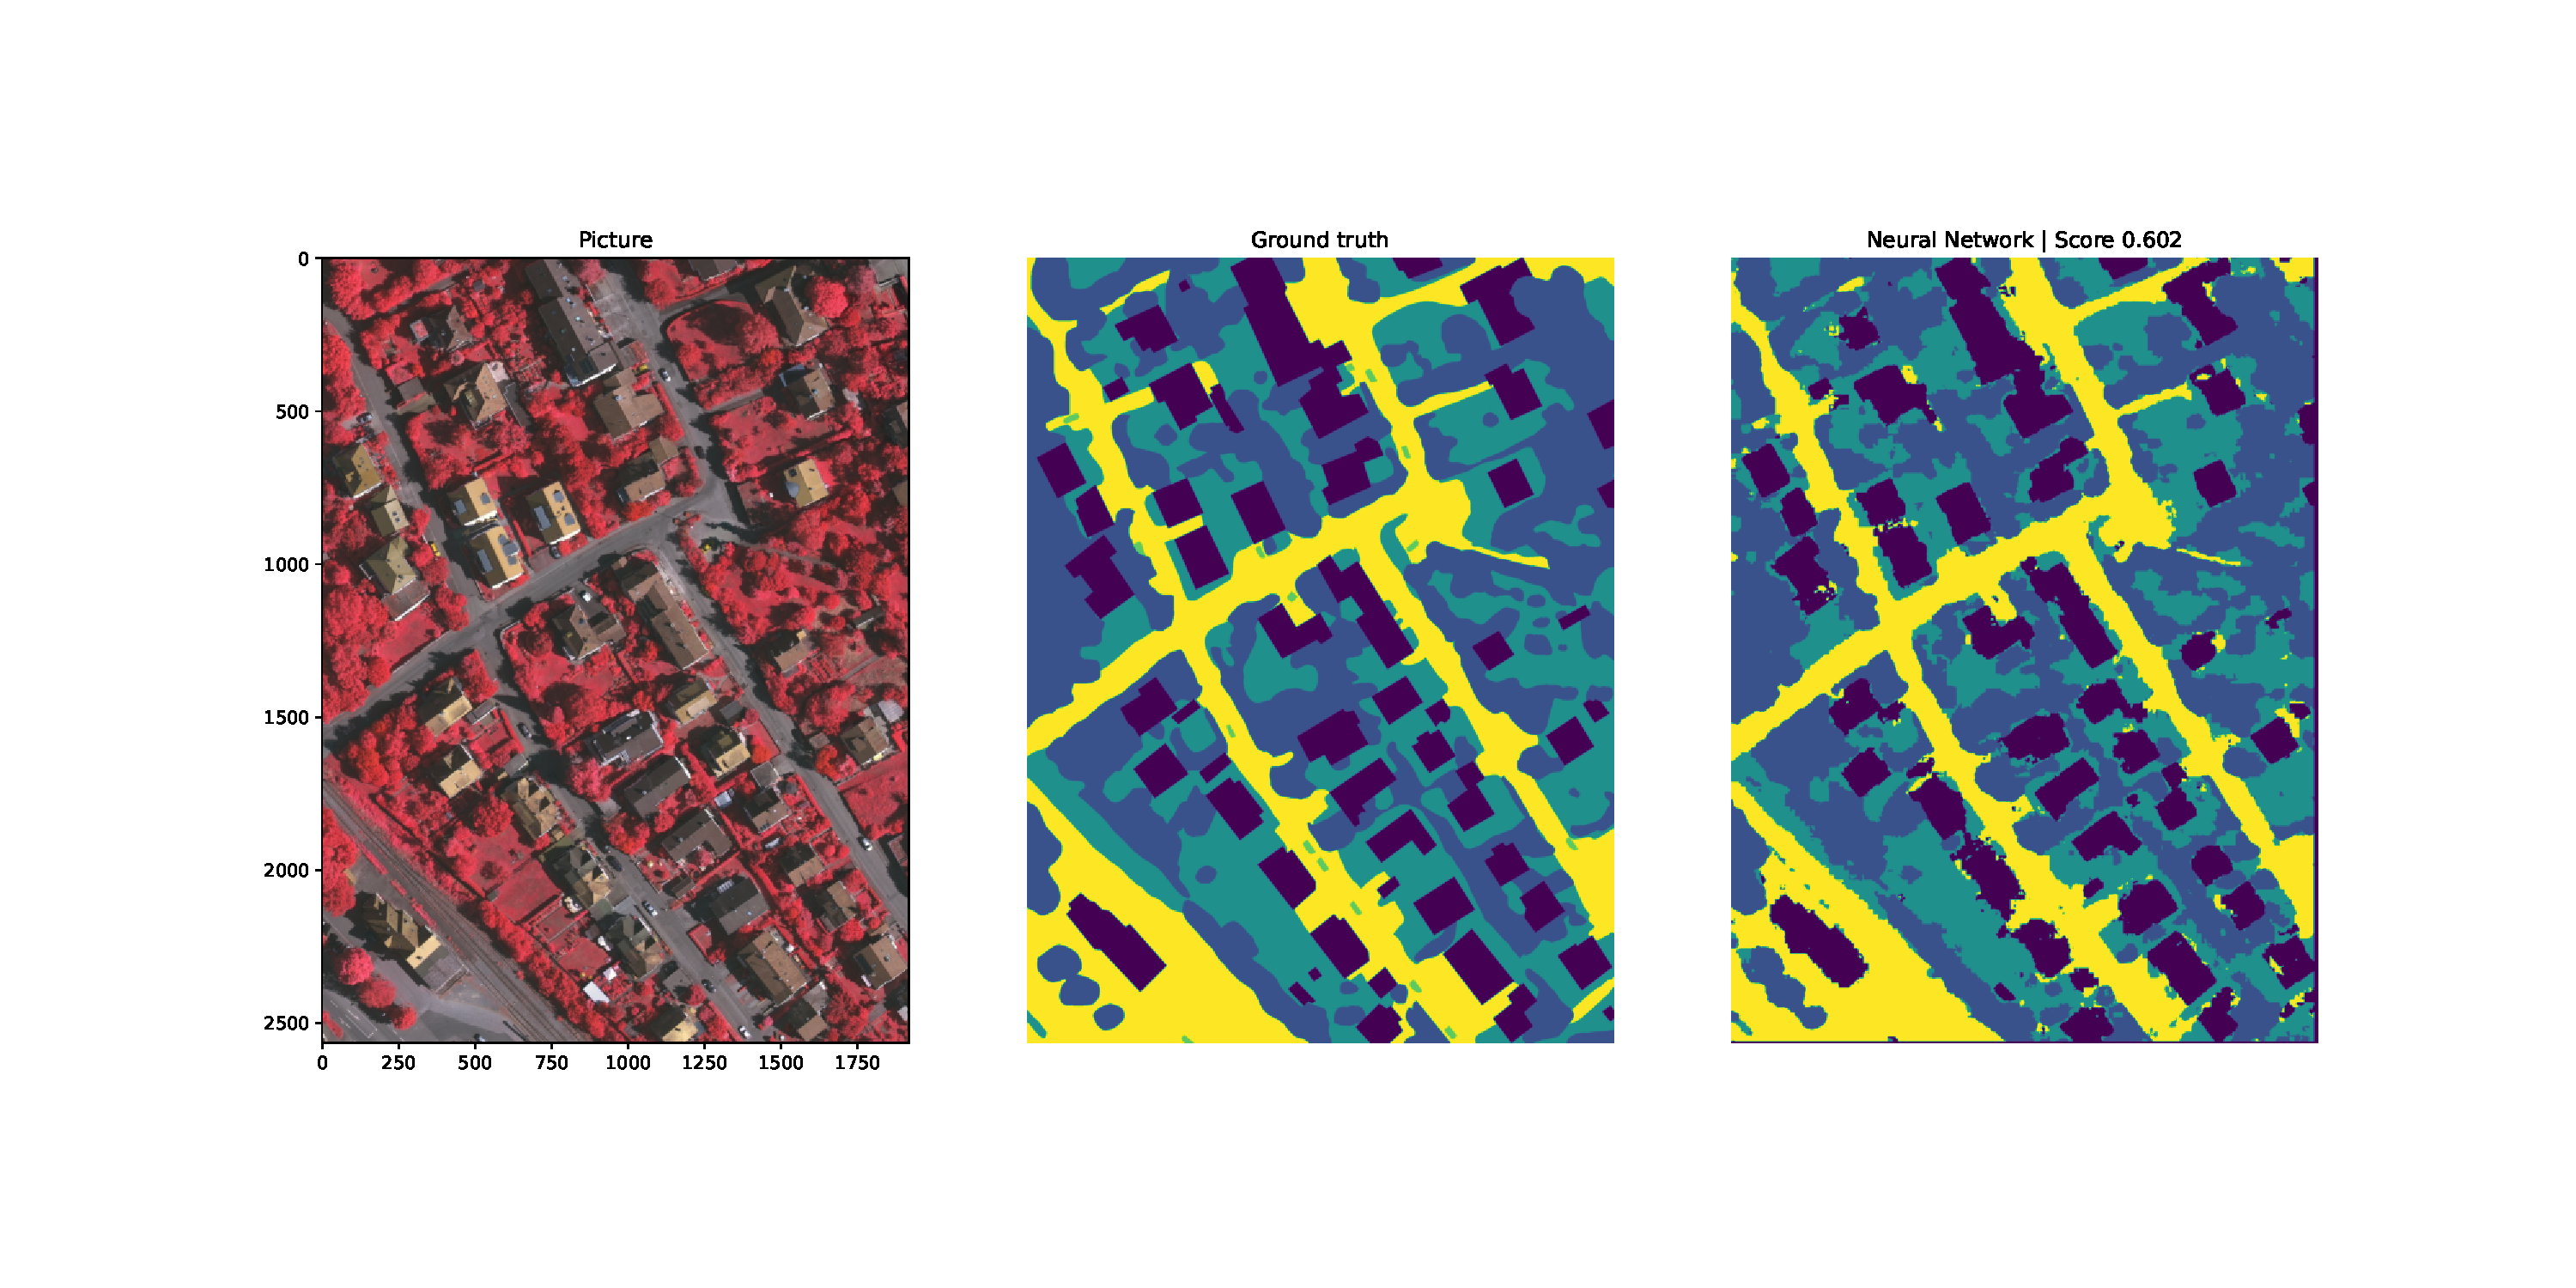
\includegraphics[width=\textwidth]{images/Patch32_imagenet_train.pdf}
      \caption{Train results}
      \label{fig:q1a_train}
  \end{subfigure}
  \hspace{0.05\textwidth}
  \begin{subfigure}[b]{0.45\textwidth}
    \centering
    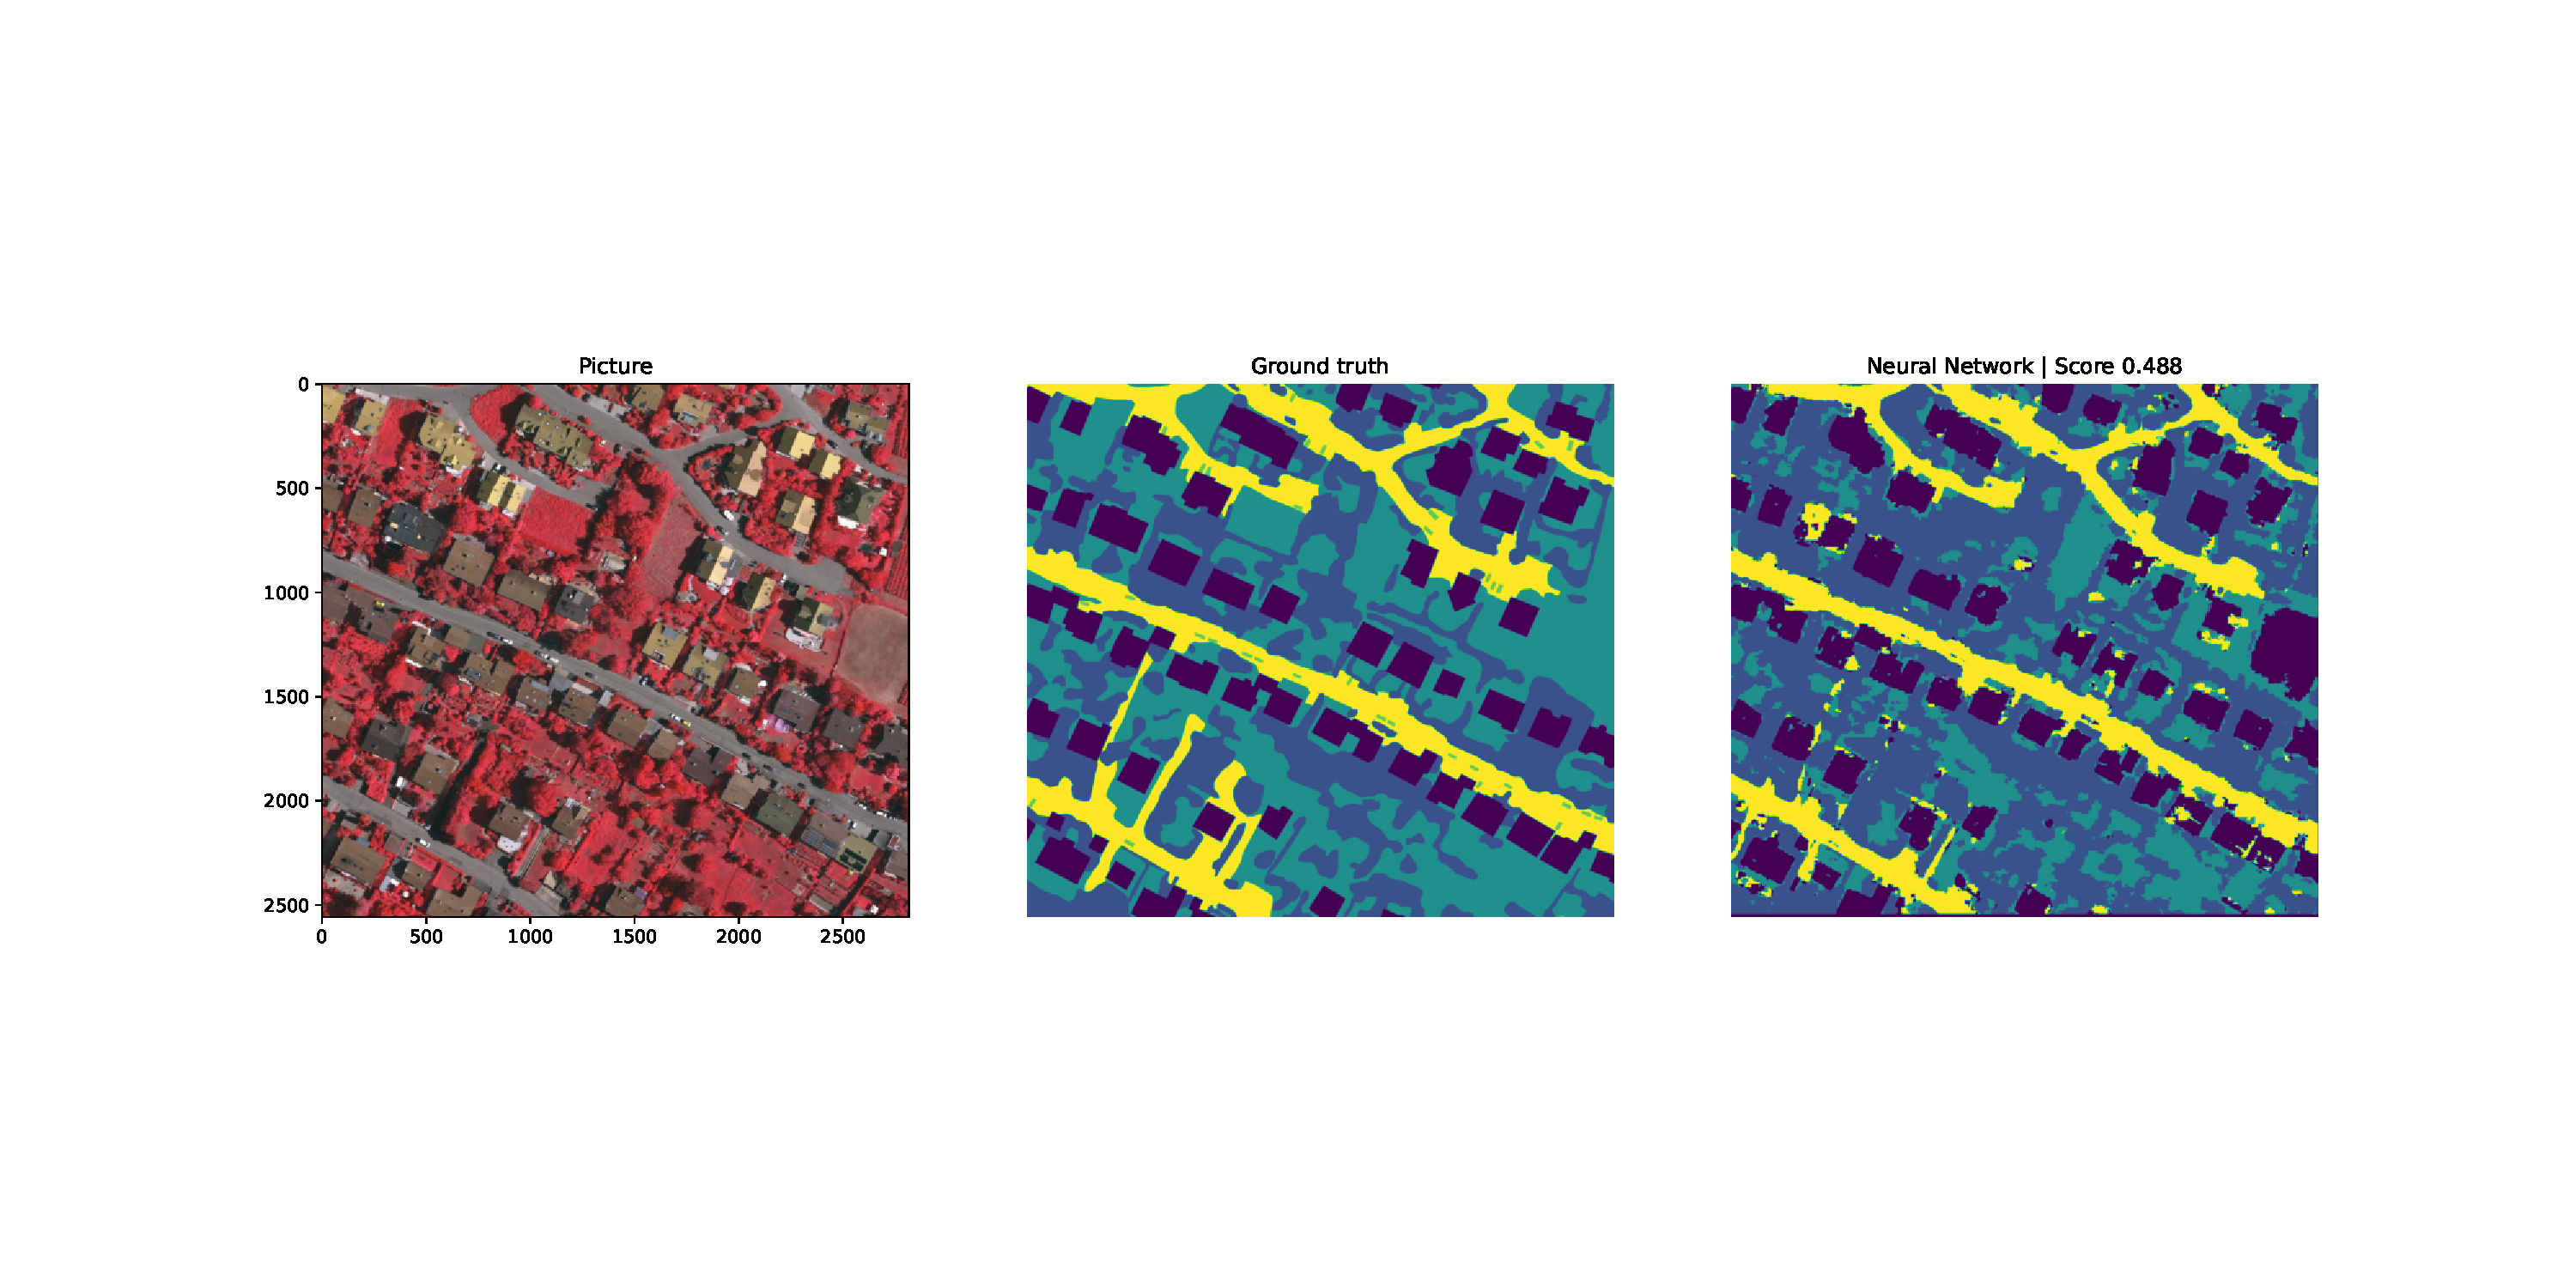
\includegraphics[width=\textwidth]{images/Patch32_imagenet_test.pdf}
    \caption{test results}
    \label{fig:q1a_test}
  \end{subfigure}
  \caption{Results of predictions for item \ref{item:1a}}
  \label{fig:q1a_results}
\end{figure}

\subsection{Item \ref{item:1b}}

Figure \ref{fig:q1b_metrics} shows the convergency of the 20 epochs using the ImageNet weights as initialization and dividing the train image into 64 x 64 patches 
with a stride of 16 pixels. As compared to case \ref{item:1a}, the same conclusions can be taken from this test, together with a general improvement in the metrics 
results.

\begin{figure}[htpb]
  \centering
  \begin{subfigure}[b]{0.32\textwidth}
      \centering
      
\includegraphics[width=\textwidth]{images/Patch64_imagenet_loss.pdf}
      \caption{Loss evolution}
      \label{fig:q1b_loss}
  \end{subfigure}
  \hfill
  \begin{subfigure}[b]{0.32\textwidth}
    \centering
    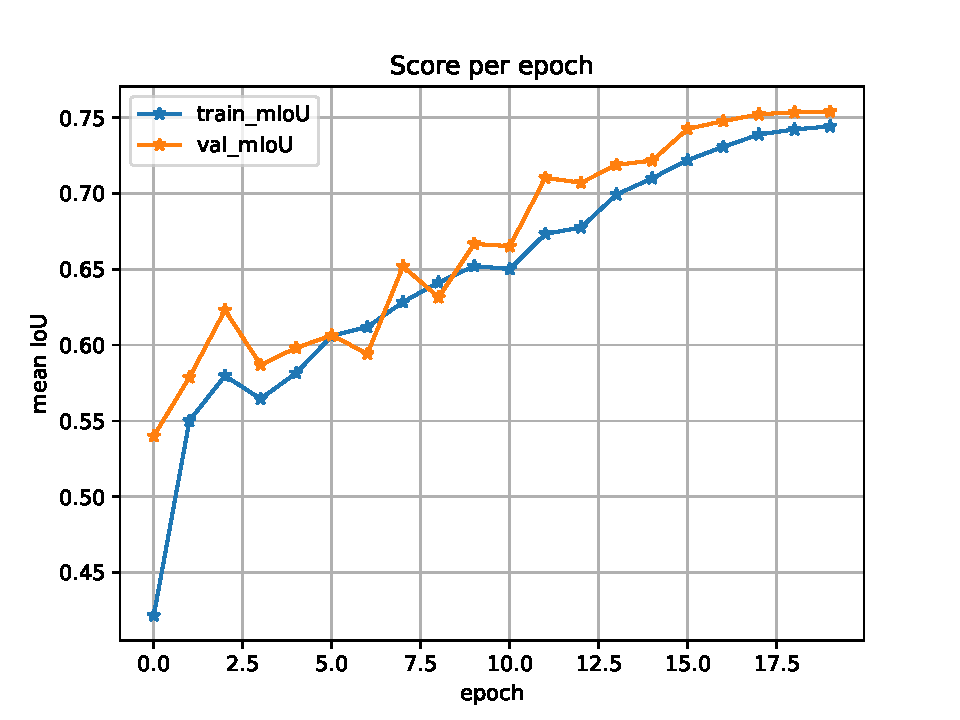
\includegraphics[width=\textwidth]{images/Patch64_imagenet_score.pdf}
    \caption{Score evolution}
    \label{fig:q1b_score}
  \end{subfigure}
  \hfill
  \begin{subfigure}[b]{0.32\textwidth}
      \centering
      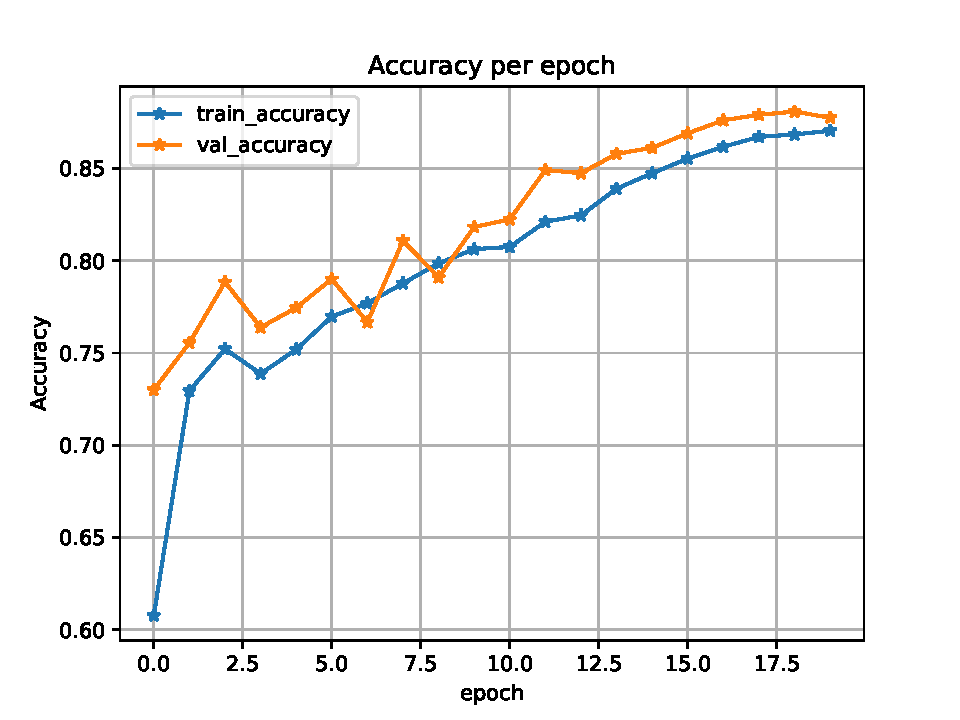
\includegraphics[width=\textwidth]{images/Patch64_imagenet_acc.pdf}
      \caption{Accuracy evolution}
      \label{fig:q1b_acc}
  \end{subfigure}
  \caption{Metrics evolution during training for item \ref{item:1b}}
  \label{fig:q1b_metrics}
\end{figure}

In figure \ref{fig:q1b_results} we see a comparison of the results obtained by running a prediction in the train and test datasets. The error metric indicated
in the image is the mean IoU between the classes. Once again, the conclusions from the test \ref{item:1a} are still valid, with the comment on the improvement
in performance and specially better separation between classes 1 and 2.

\begin{figure}[htpb]
  \centering
  \begin{subfigure}[b]{0.45\textwidth}
      \centering
      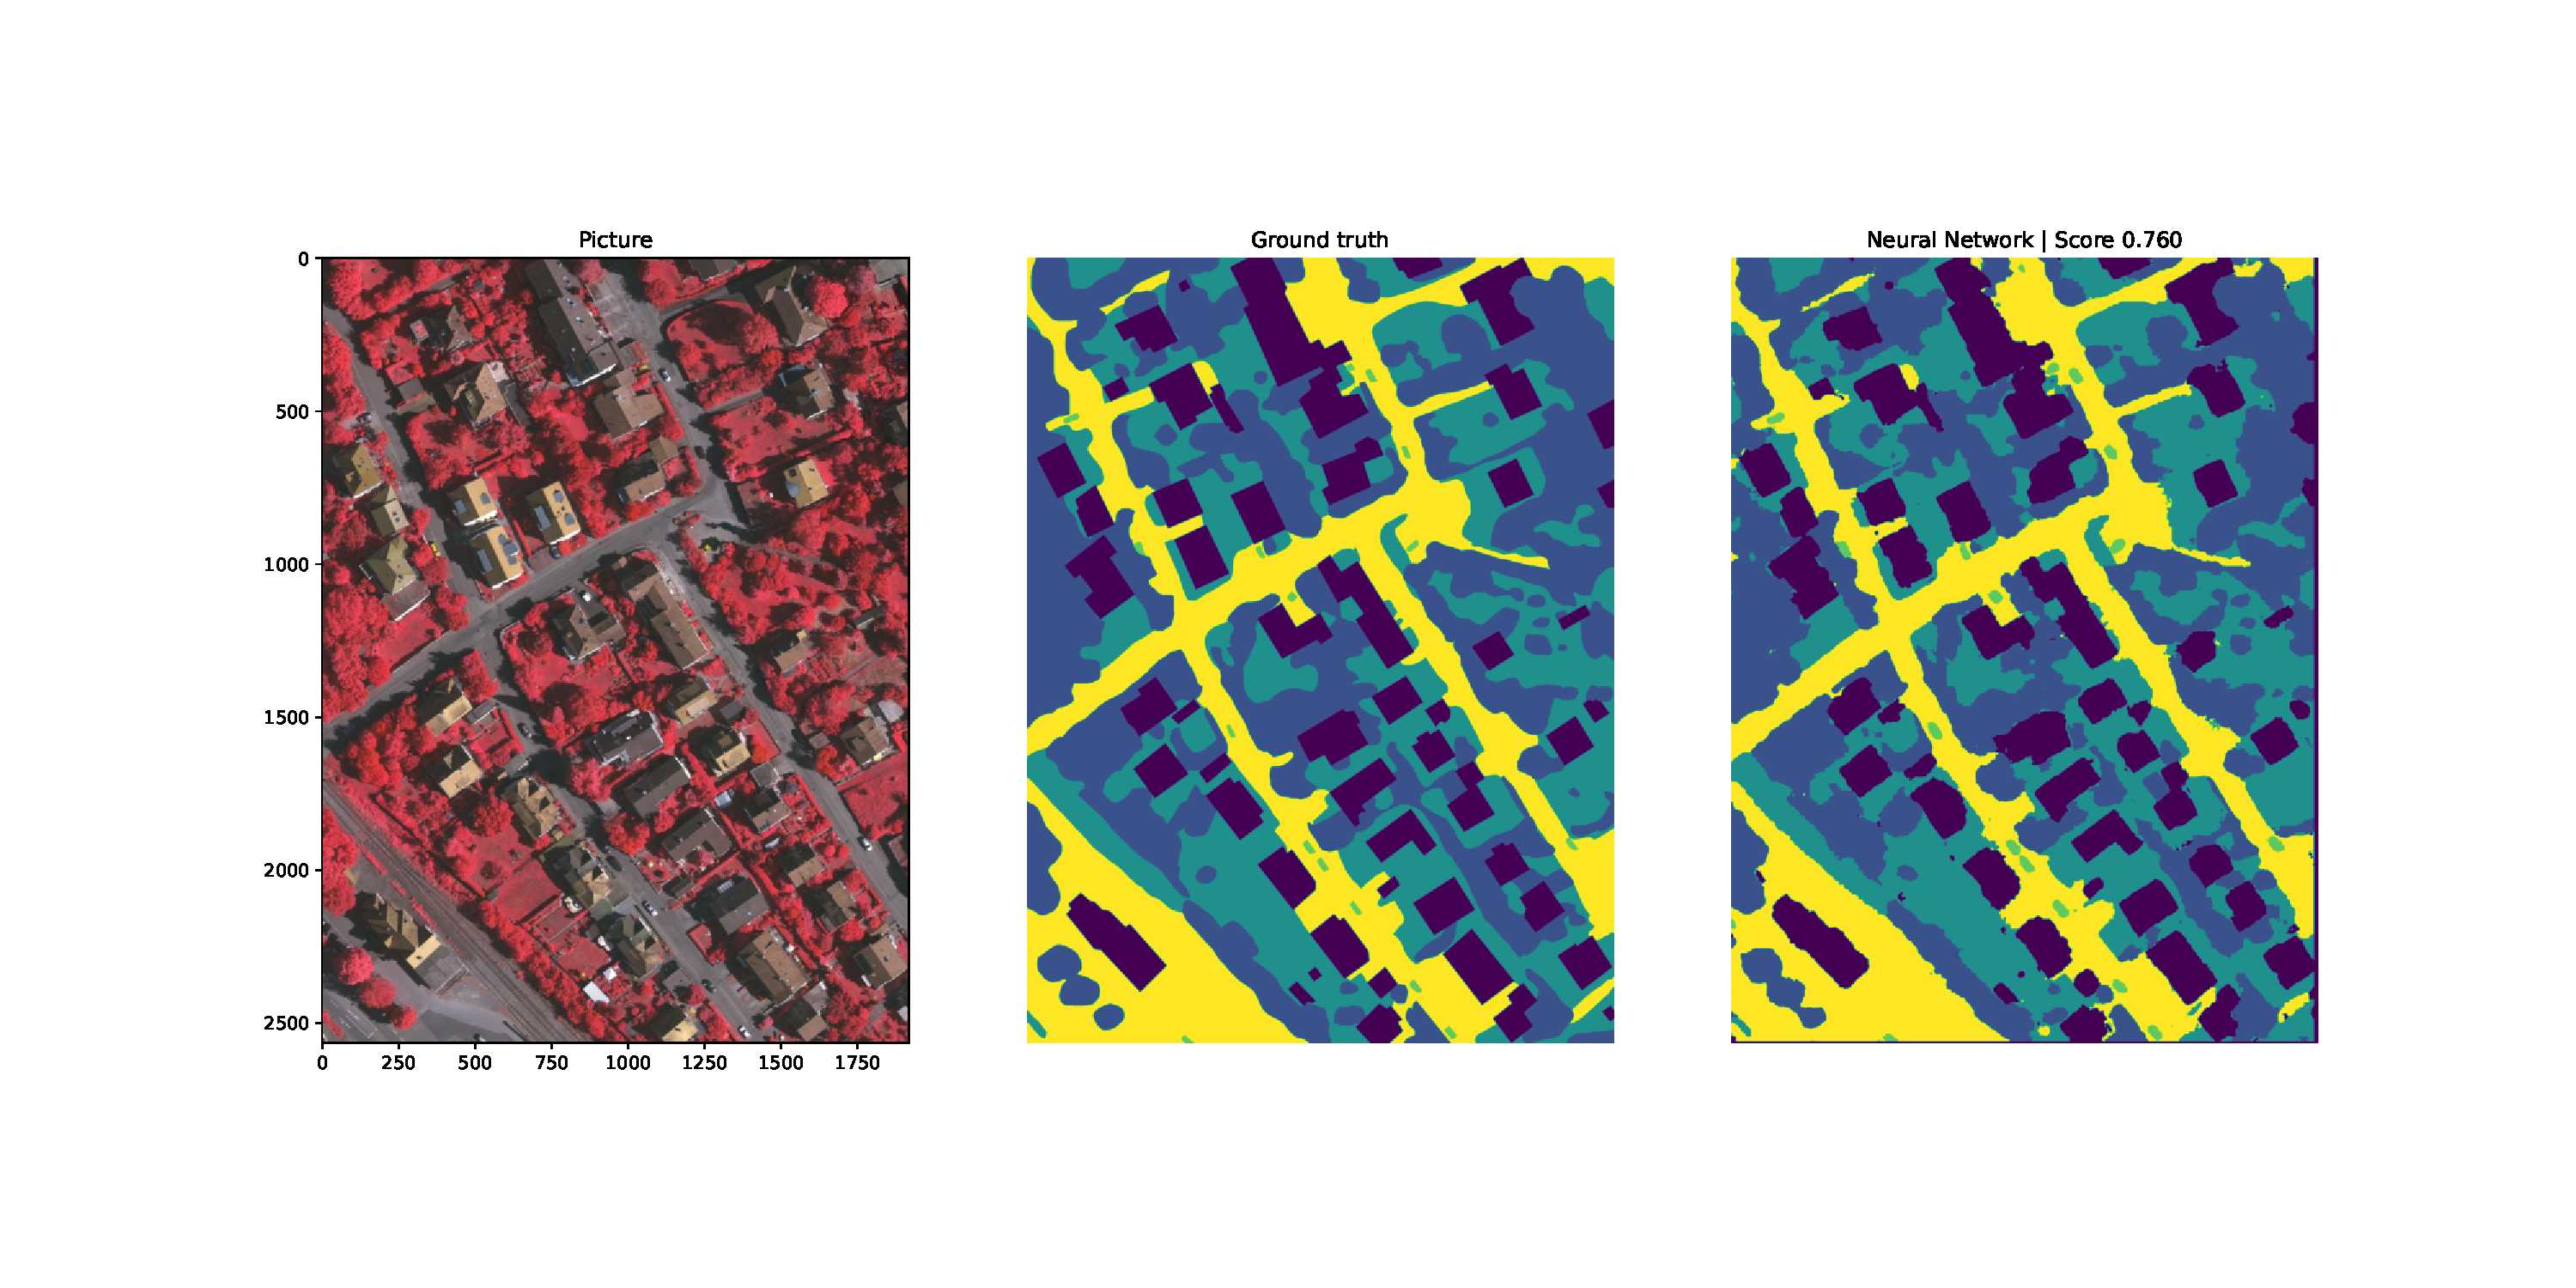
\includegraphics[width=\textwidth]{images/Patch64_imagenet_train.pdf}
      \caption{Train results}
      \label{fig:q1b_train}
  \end{subfigure}
  \hspace{0.05\textwidth}
  \begin{subfigure}[b]{0.45\textwidth}
    \centering
    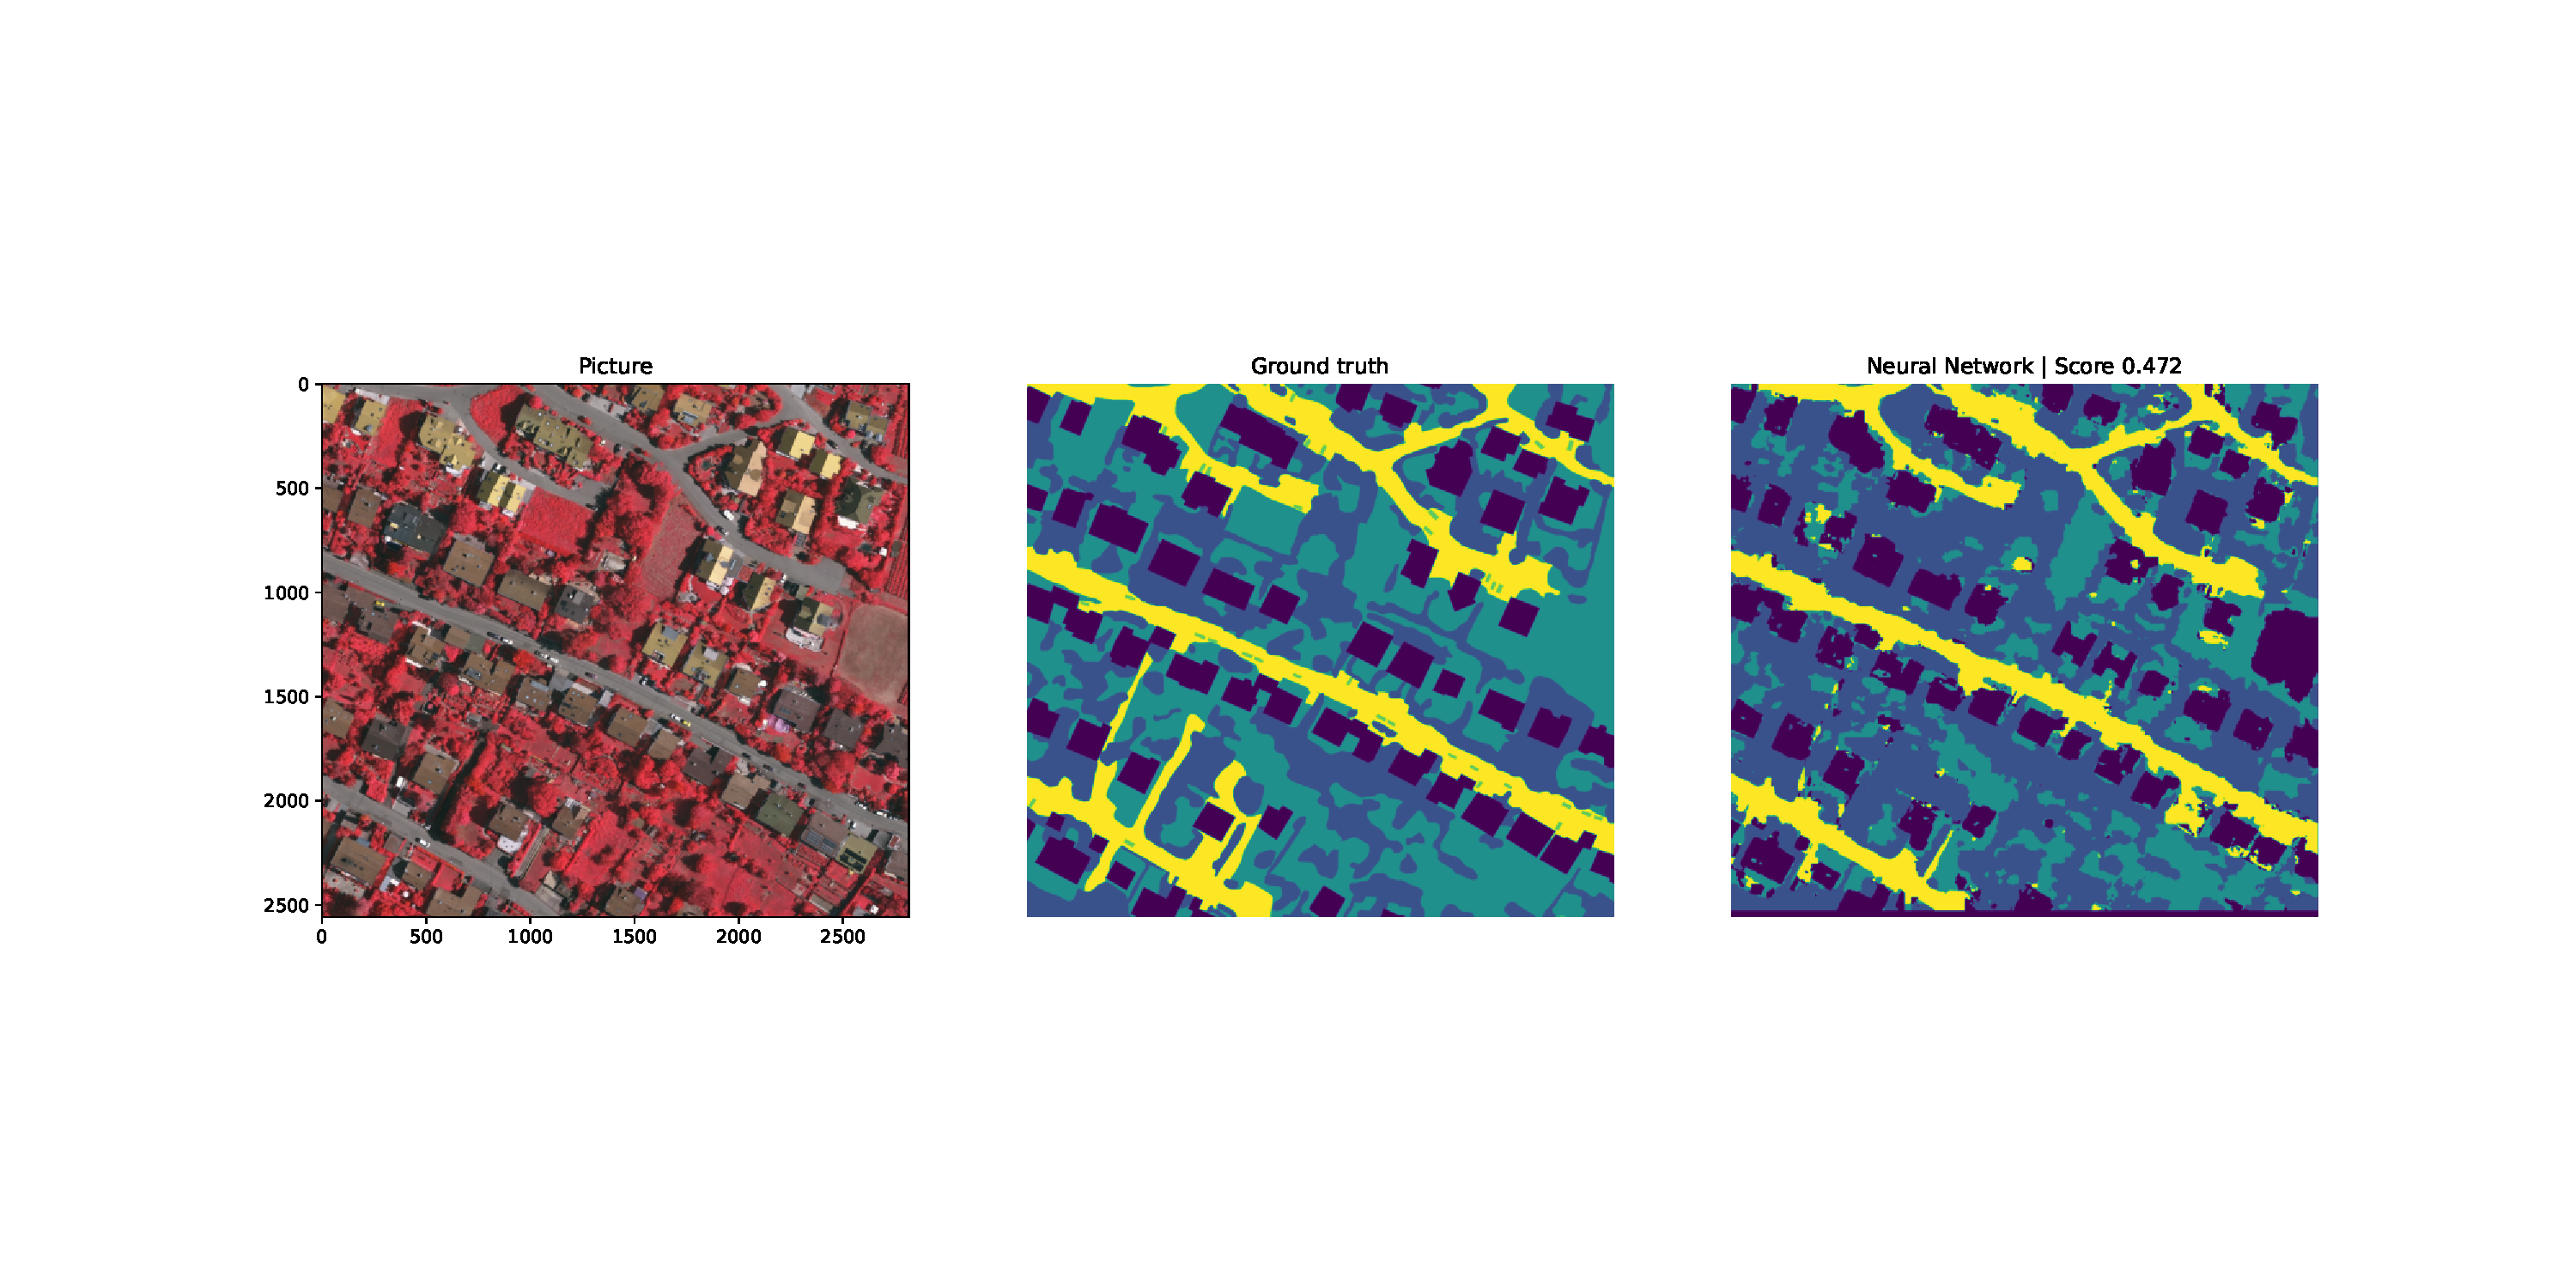
\includegraphics[width=\textwidth]{images/Patch64_imagenet_test.pdf}
    \caption{test results}
    \label{fig:q1b_test}
  \end{subfigure}
  \caption{Results of predictions for item \ref{item:1b}}
  \label{fig:q1b_results}
\end{figure}

\subsection{Item \ref{item:1c}}

Figure \ref{fig:q1c_metrics} shows the convergency of the 20 epochs using the ImageNet weights as initialization and dividing the train image into 128 x 128 patches 
with a stride of 16 pixels. Once again, as compared to cases \ref{item:1a} and \ref{item:1b}, the same conclusions can be taken from this test, together with a general improvement in the metrics 
results.

\begin{figure}[htpb]
  \centering
  \begin{subfigure}[b]{0.32\textwidth}
      \centering
      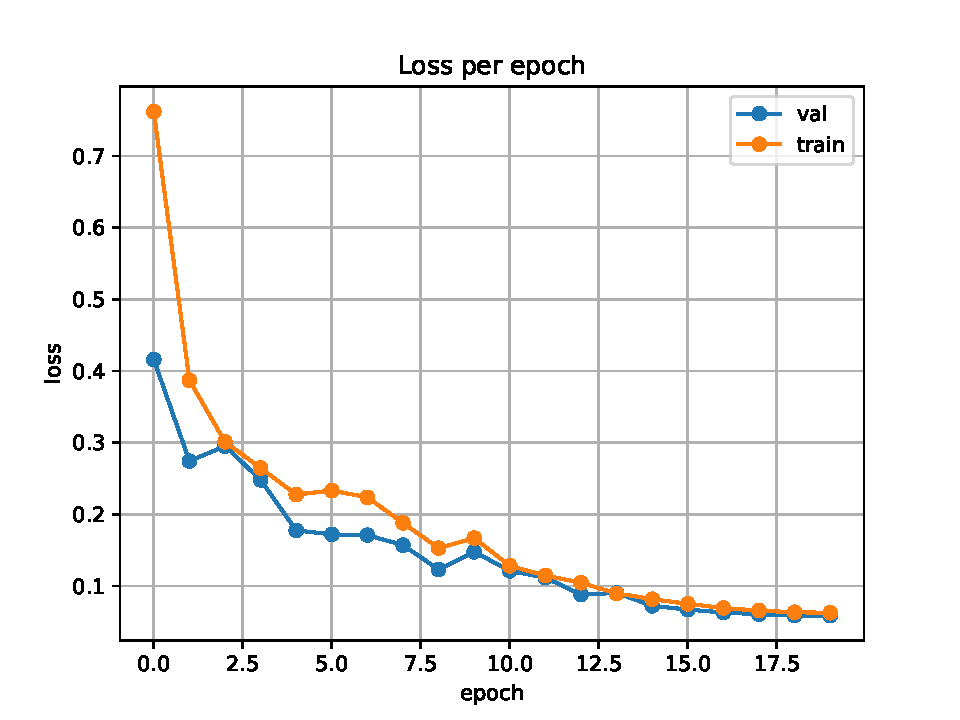
\includegraphics[width=\textwidth]{images/Patch128_imagenet_loss.pdf}
      \caption{Loss evolution}
      \label{fig:q1c_loss}
  \end{subfigure}
  \hfill
  \begin{subfigure}[b]{0.32\textwidth}
    \centering
    
\includegraphics[width=\textwidth]{images/Patch128_imagenet_score.pdf}
    \caption{Score evolution}
    \label{fig:q1c_score}
  \end{subfigure}
  \hfill
  \begin{subfigure}[b]{0.32\textwidth}
      \centering
      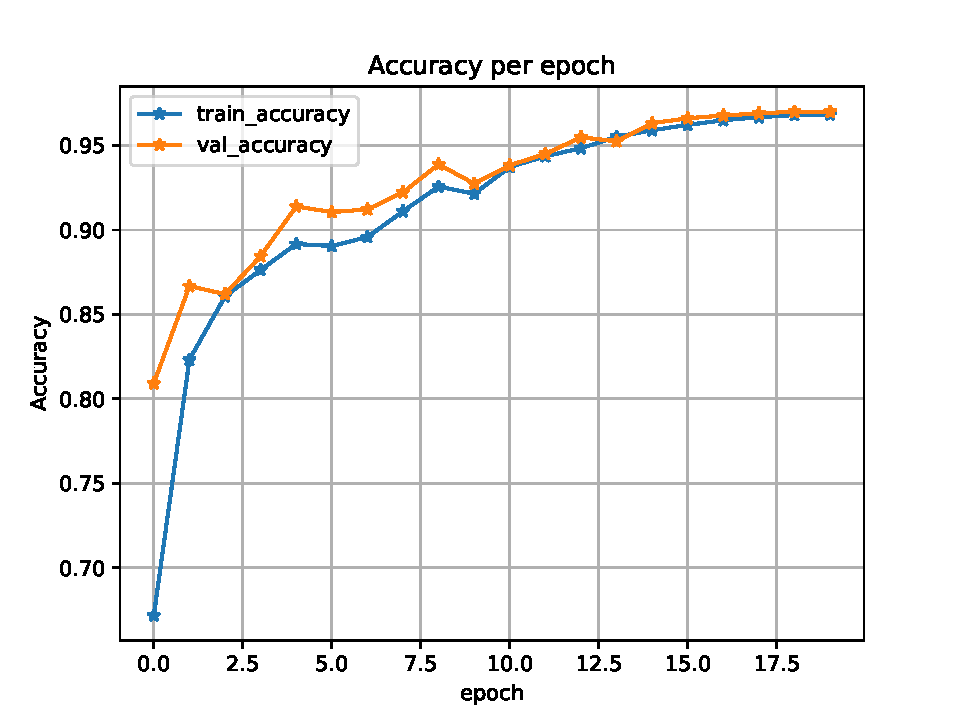
\includegraphics[width=\textwidth]{images/Patch128_imagenet_acc.pdf}
      \caption{Accuracy evolution}
      \label{fig:q1c_acc}
  \end{subfigure}
  \caption{Metrics evolution during training for item \ref{item:1c}}
  \label{fig:q1c_metrics}
\end{figure}

In figure \ref{fig:q1b_results} we see a comparison of the results obtained by running a prediction in the train and test datasets. The error metric indicated
in the image is the mean IoU between the classes. Same conclusions from the previous cases can be drawn from this test.

\begin{figure}[htpb]
  \centering
  \begin{subfigure}[b]{0.45\textwidth}
      \centering
      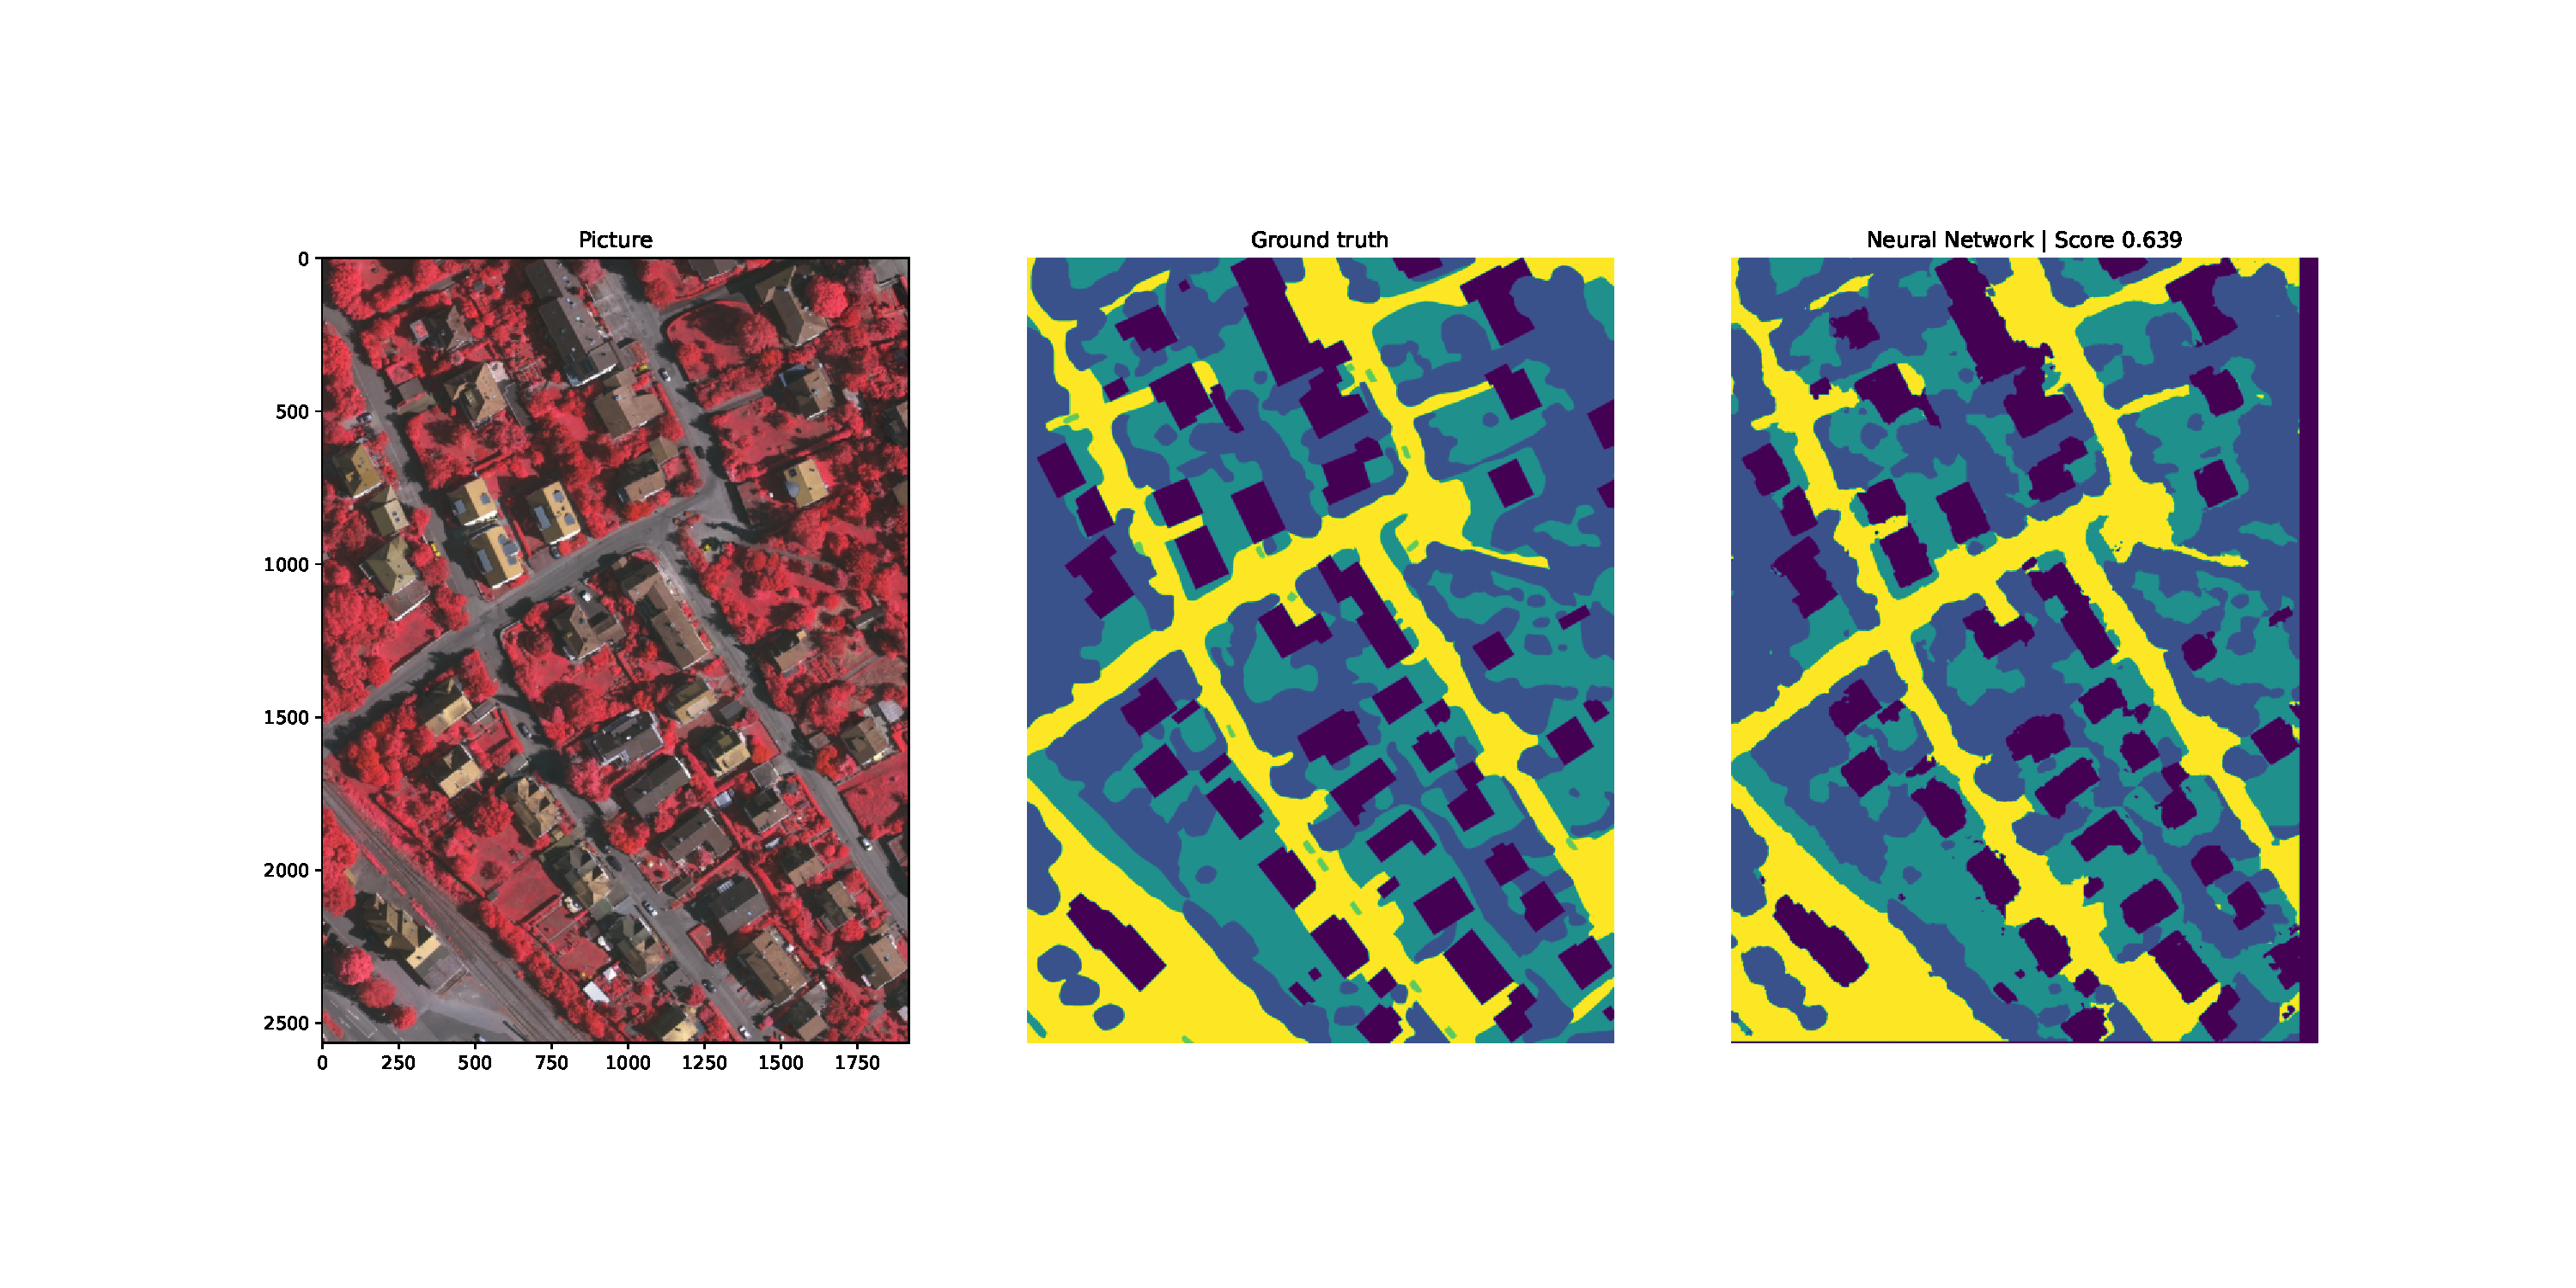
\includegraphics[width=\textwidth]{images/Patch128_imagenet_train.pdf}
      \caption{Train results}
      \label{fig:q1c_train}
  \end{subfigure}
  \hspace{0.05\textwidth}
  \begin{subfigure}[b]{0.45\textwidth}
    \centering
    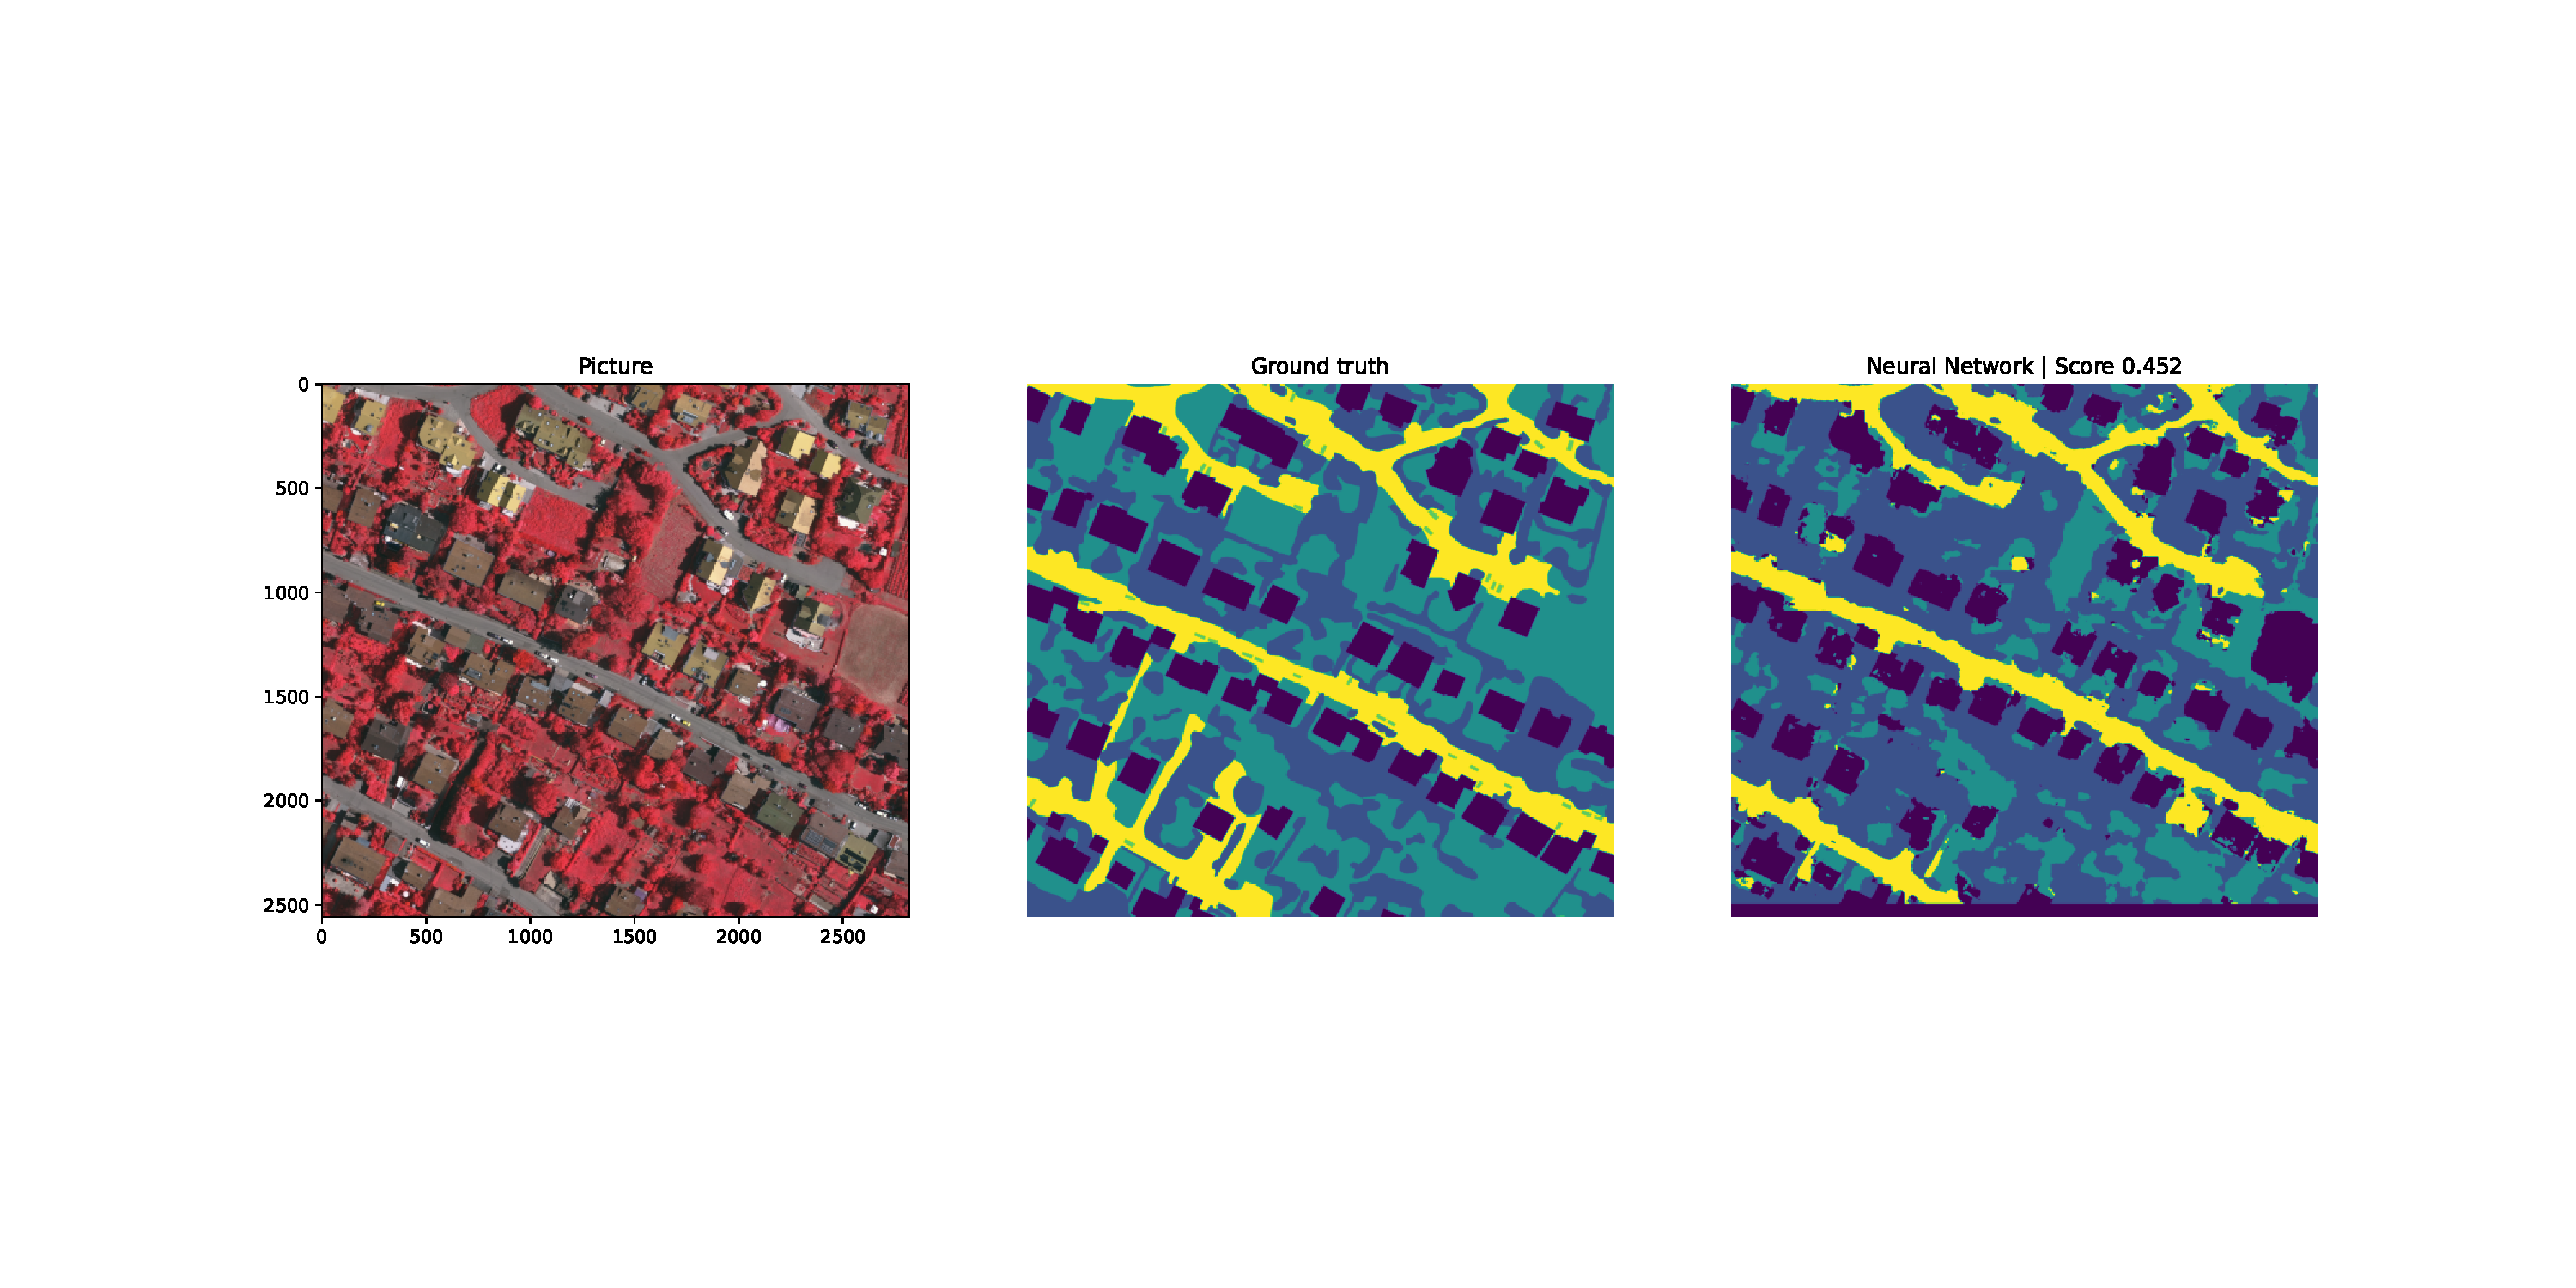
\includegraphics[width=\textwidth]{images/Patch128_imagenet_test.pdf}
    \caption{test results}
    \label{fig:q1c_test}
  \end{subfigure}
  \caption{Results of predictions for item \ref{item:1c}}
  \label{fig:q1c_results}
\end{figure}

\newpage
\subsection{Item \ref{item:2a}}

Figure \ref{fig:q2a_metrics} shows the convergency of the 20 epochs using the random weights as initialization and dividing the train image into 32 x 32 patches 
with a stride of 16 pixels. Overall, the results are similar to the case \ref{item:1a}, but is noticeable a worse performence of this initial weights. Perhaps this
could be mitigated by allowing more training epochs, but it does not seem to be the case since the aspect of the convergency is similar to the one displayed in
Figure \ref{fig:q1a_metrics}

\begin{figure}[htpb]
  \centering
  \begin{subfigure}[b]{0.32\textwidth}
      \centering
      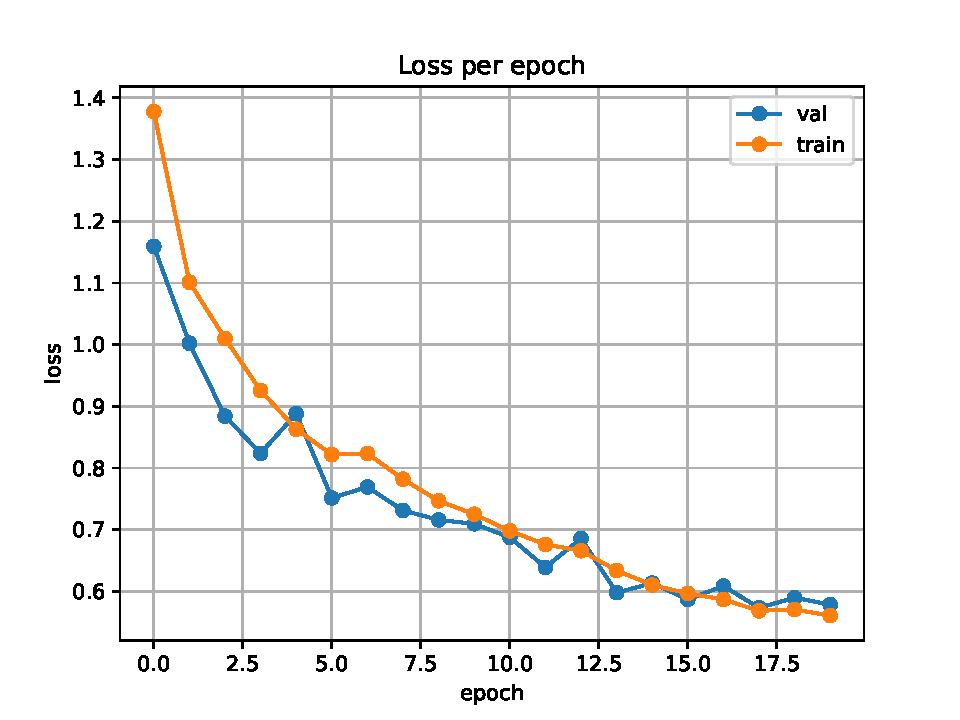
\includegraphics[width=\textwidth]{images/Patch32_scratch_loss.pdf}
      \caption{Loss evolution}
      \label{fig:q2a_loss}
  \end{subfigure}
  \hfill
  \begin{subfigure}[b]{0.32\textwidth}
    \centering
    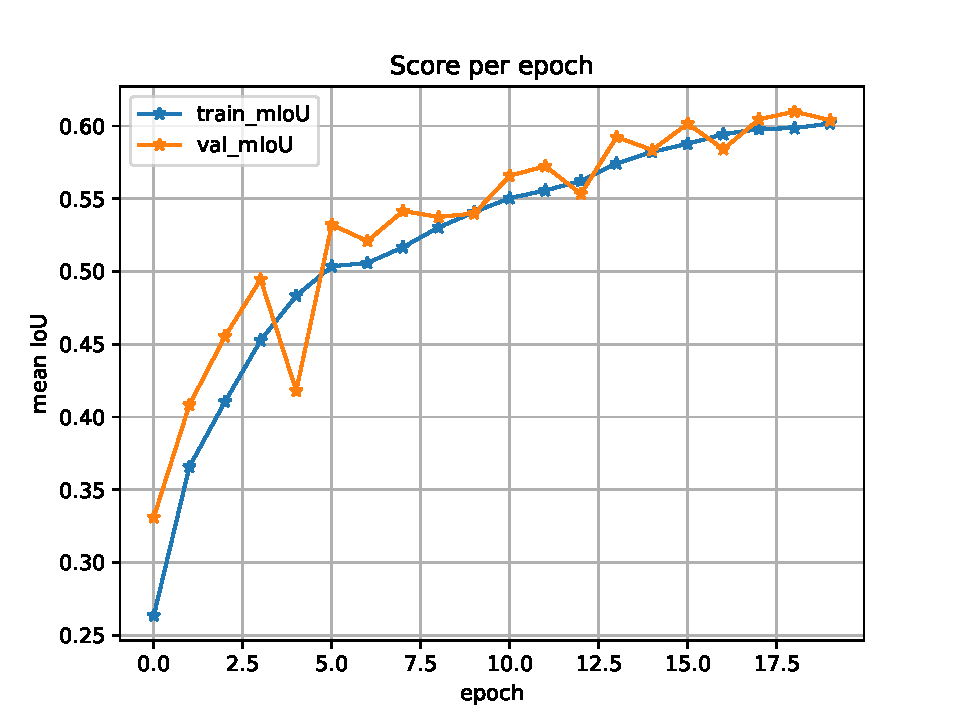
\includegraphics[width=\textwidth]{images/Patch32_scratch_score.pdf}
    \caption{Score evolution}
    \label{fig:q2a_score}
  \end{subfigure}
  \hfill
  \begin{subfigure}[b]{0.32\textwidth}
      \centering
      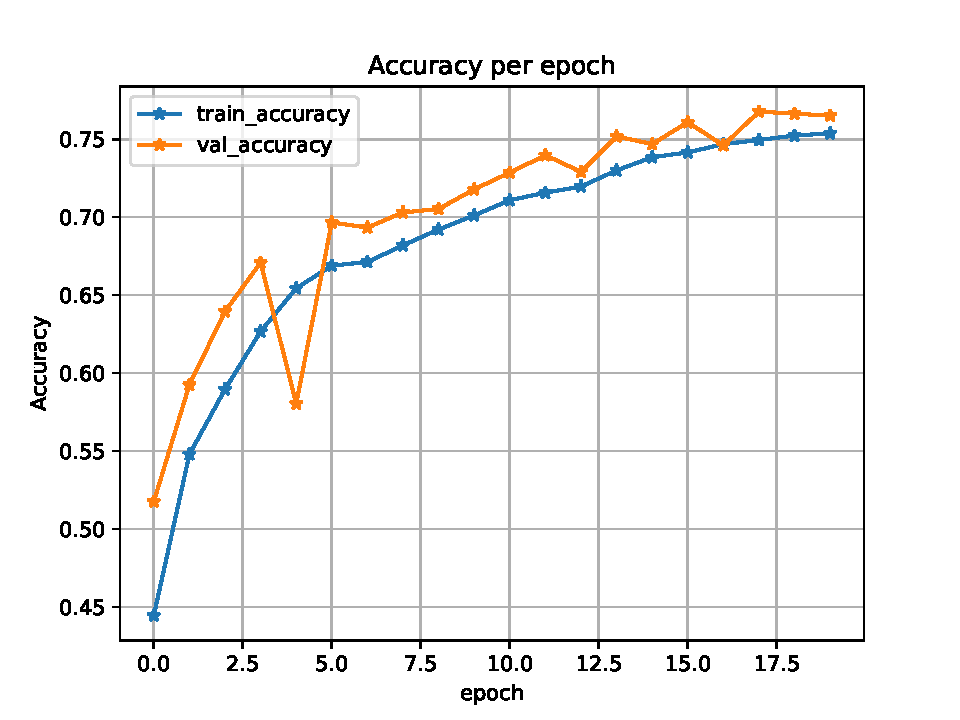
\includegraphics[width=\textwidth]{images/Patch32_scratch_acc.pdf}
      \caption{Accuracy evolution}
      \label{fig:q2a_acc}
  \end{subfigure}
  \caption{Metrics evolution during training for item \ref{item:2a}}
  \label{fig:q2a_metrics}
\end{figure}

The results obtained by running predicitions on the images nd displayed in Figure \ref{fig:q2a_results} also show a worse version of the prediction performed in
case \ref{item:1a}.

\begin{figure}[htpb]
  \centering
  \begin{subfigure}[b]{0.45\textwidth}
      \centering
      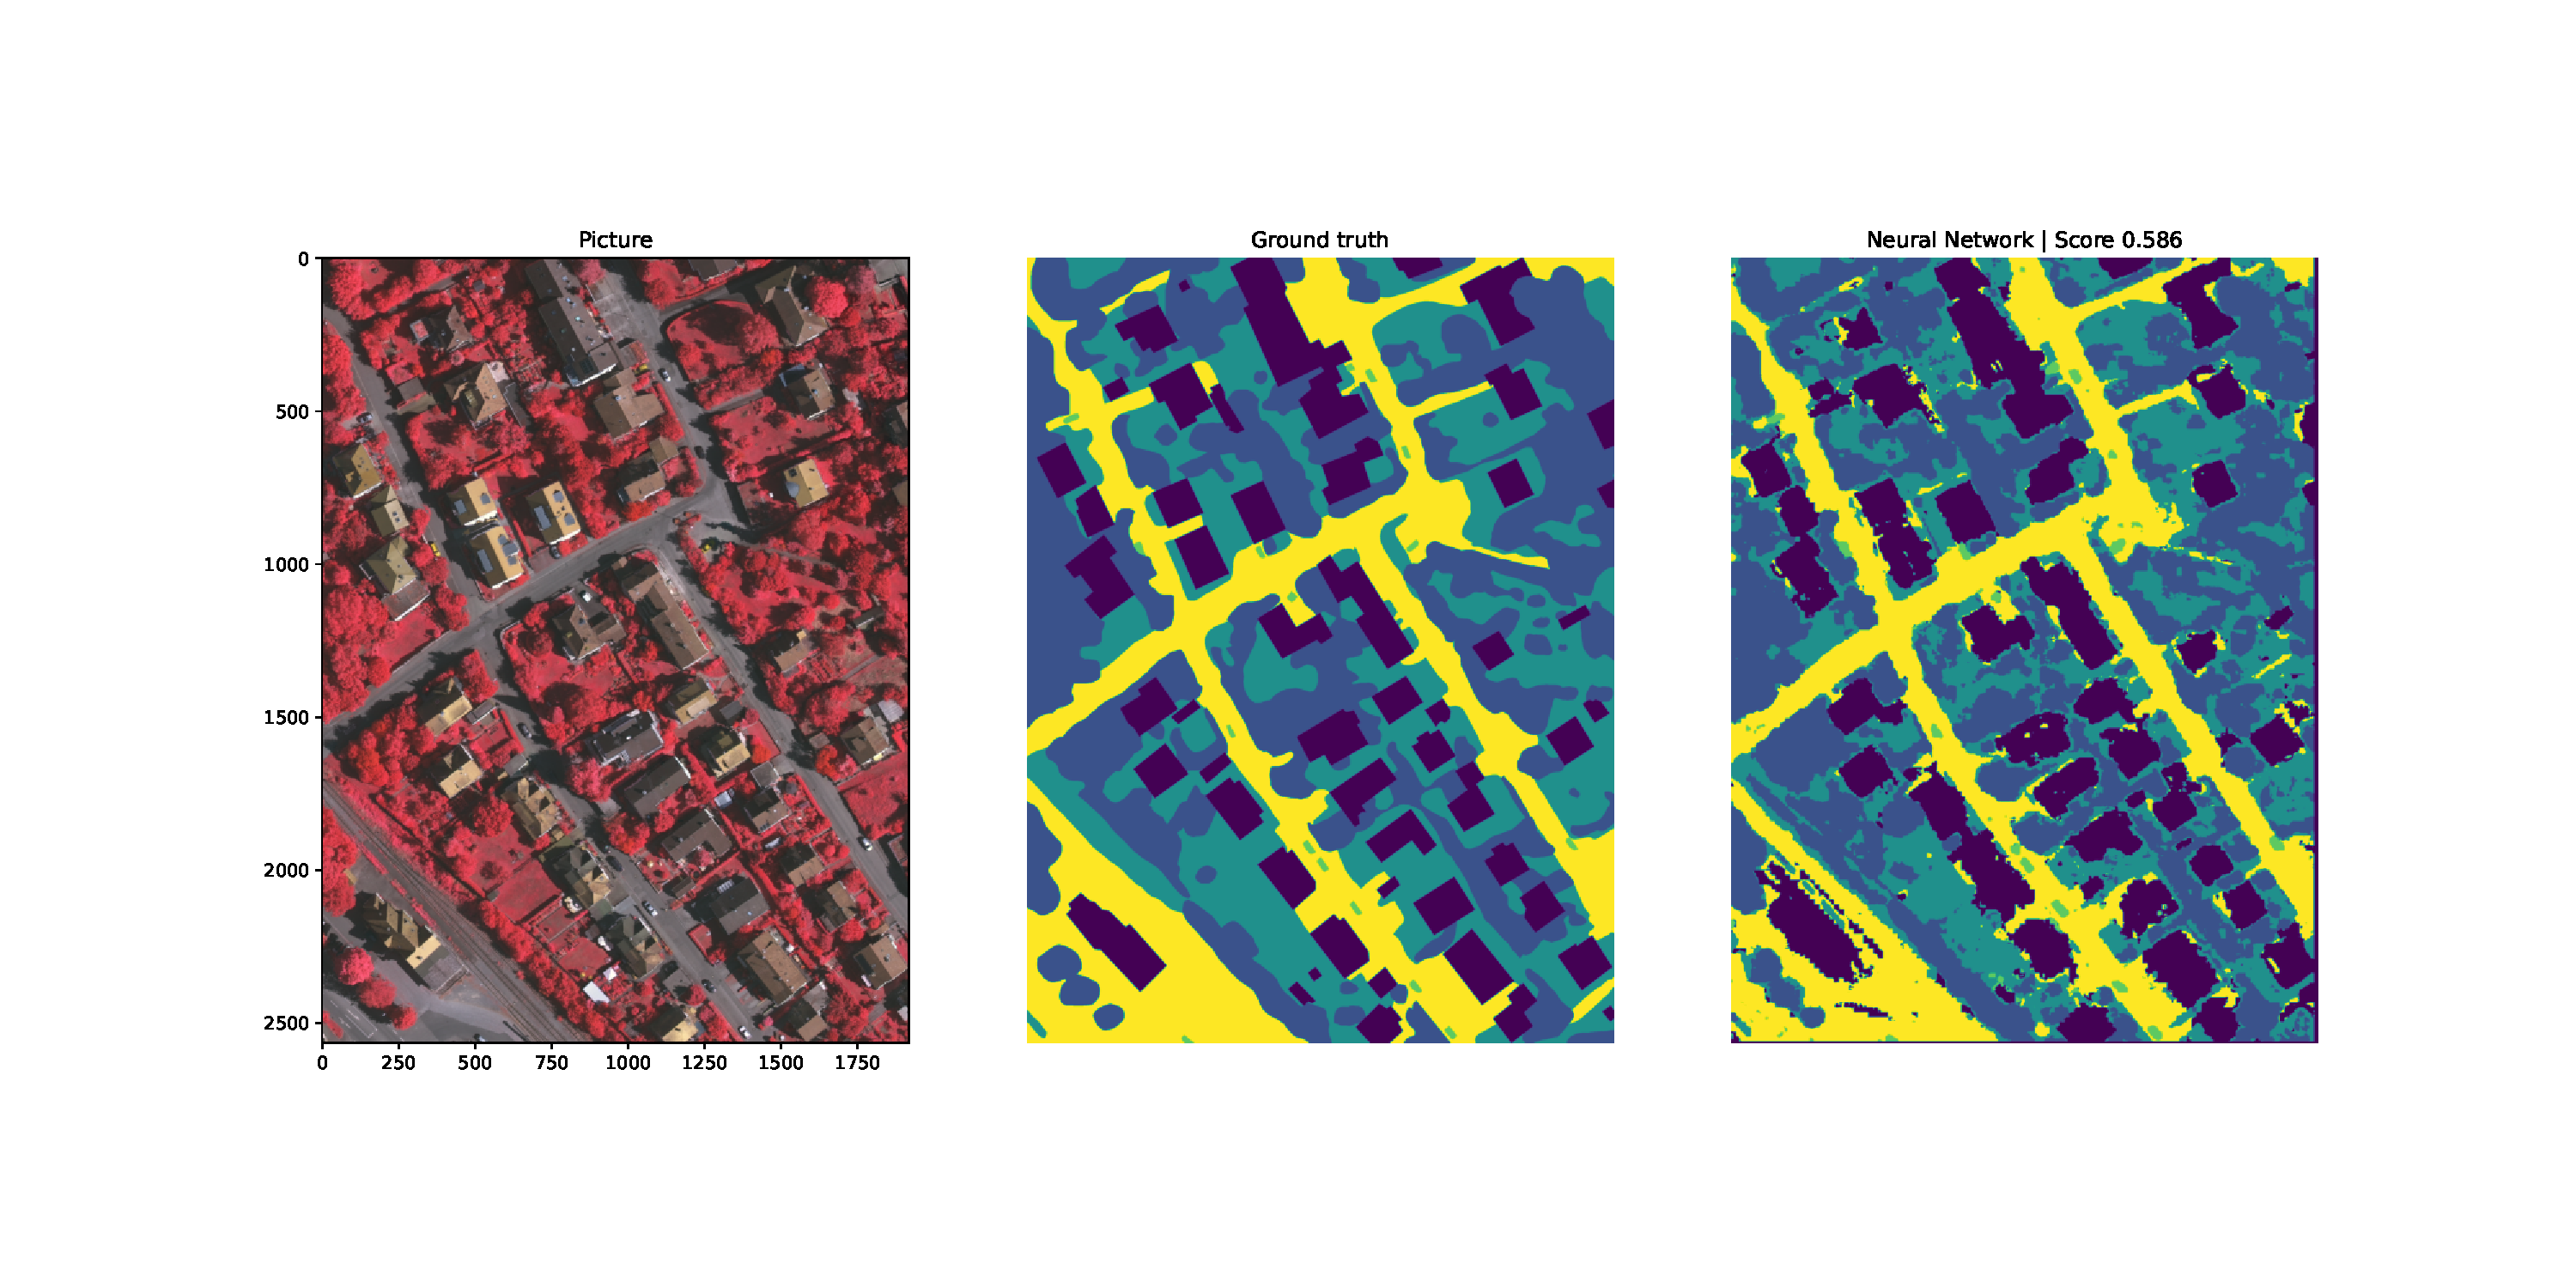
\includegraphics[width=\textwidth]{images/Patch32_scratch_train.pdf}
      \caption{Train results}
      \label{fig:q2a_train}
  \end{subfigure}
  \hspace{0.05\textwidth}
  \begin{subfigure}[b]{0.45\textwidth}
    \centering
    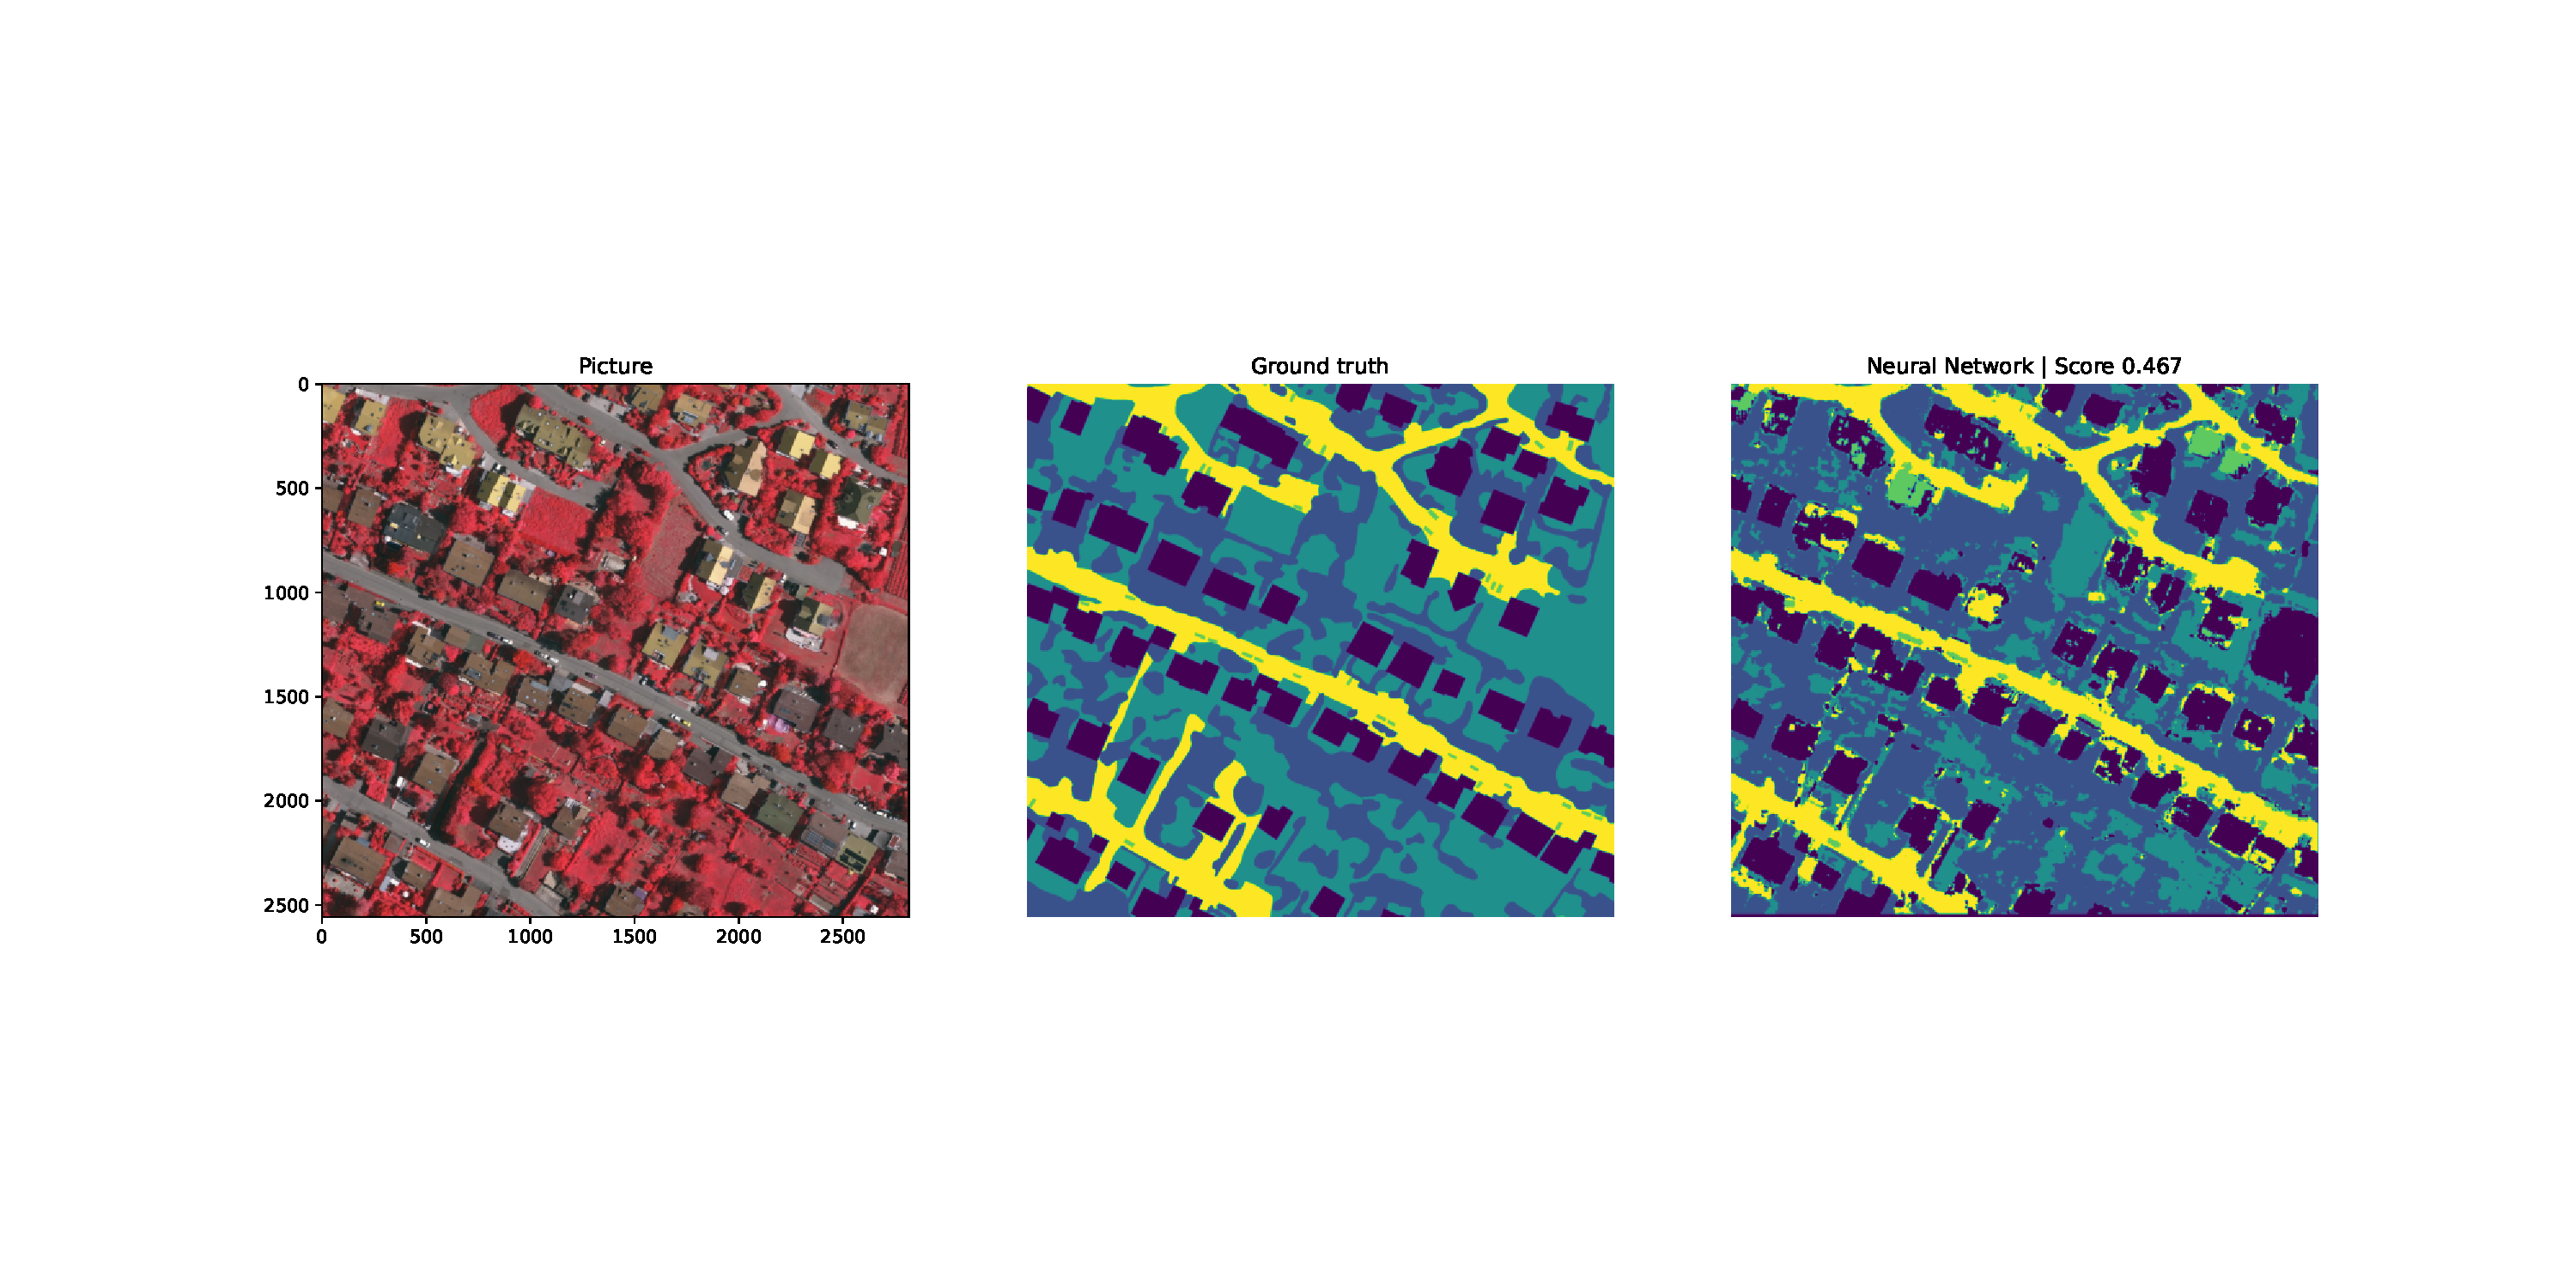
\includegraphics[width=\textwidth]{images/Patch32_scratch_test.pdf}
    \caption{test results}
    \label{fig:q2a_test}
  \end{subfigure}
  \caption{Results of predictions for item \ref{item:2a}}
  \label{fig:q2a_results}
\end{figure}

\subsection{Item \ref{item:2b}}

Figures \ref{fig:q2b_metrics} and \ref{fig:q2b_results} show the convergency of the 20 epochs and test results obtained by using the random weights as initialization 
and dividing the train image into 64 x 64 patches with a stride of 16 pixels. Once again, slightly worse results are obtained when compared to case \ref{item:1b}.

\begin{figure}[htpb]
  \centering
  \begin{subfigure}[b]{0.32\textwidth}
      \centering
      
\includegraphics[width=\textwidth]{images/Patch64_scratch_loss.pdf}
      \caption{Loss evolution}
      \label{fig:q2b_loss}
  \end{subfigure}
  \hfill
  \begin{subfigure}[b]{0.32\textwidth}
    \centering
    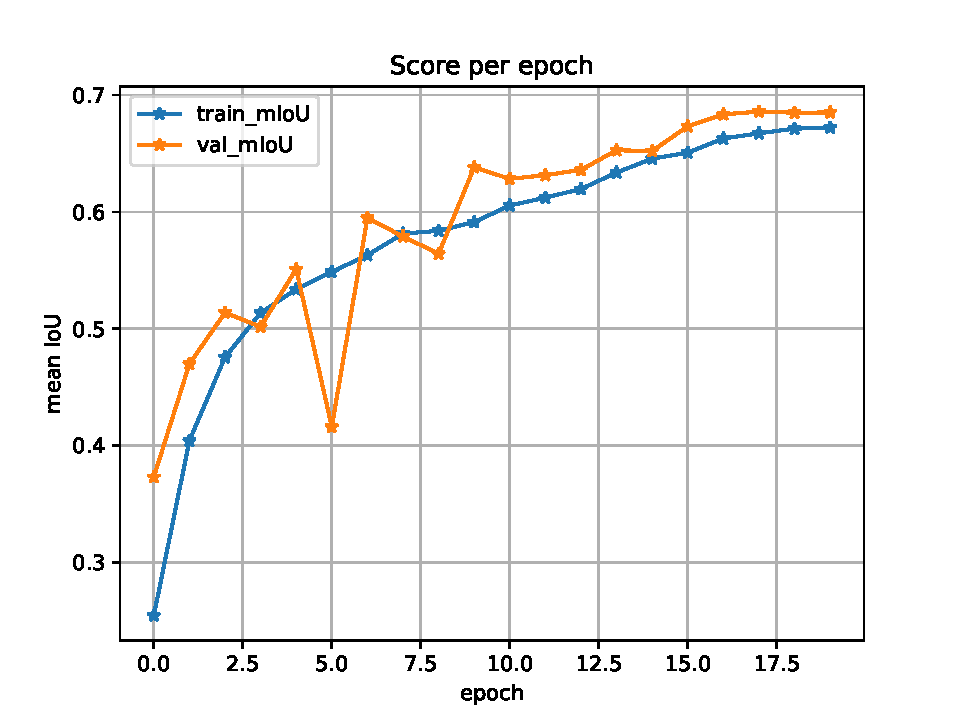
\includegraphics[width=\textwidth]{images/Patch64_scratch_score.pdf}
    \caption{Score evolution}
    \label{fig:q2b_score}
  \end{subfigure}
  \hfill
  \begin{subfigure}[b]{0.32\textwidth}
      \centering
      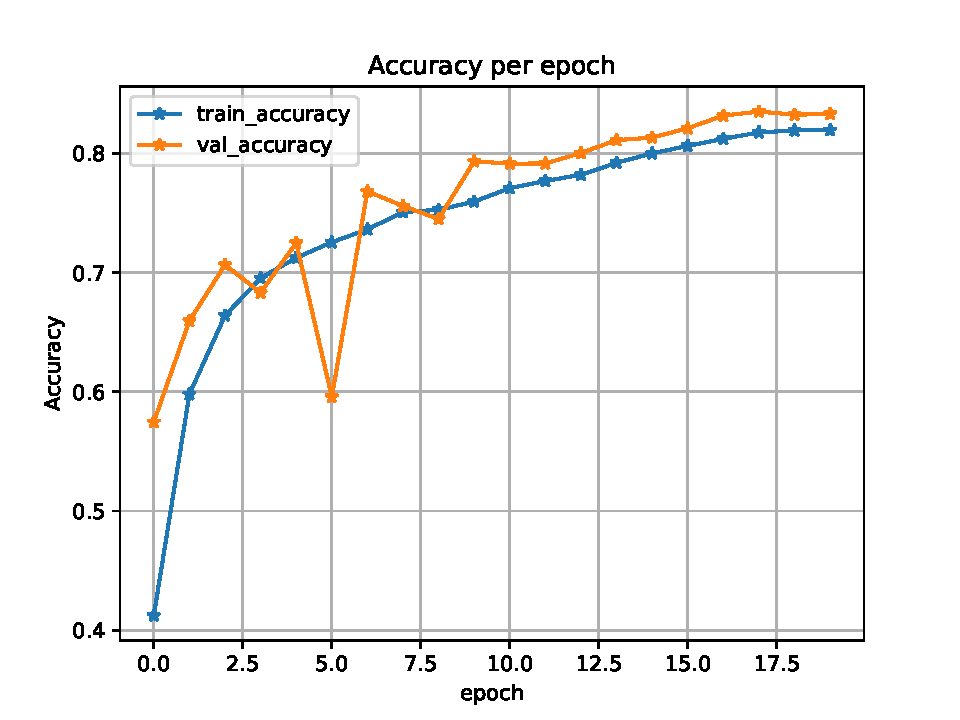
\includegraphics[width=\textwidth]{images/Patch64_scratch_acc.pdf}
      \caption{Accuracy evolution}
      \label{fig:q2b_acc}
  \end{subfigure}
  \caption{Metrics evolution during training for item \ref{item:2b}}
  \label{fig:q2b_metrics}
\end{figure}

\begin{figure}[htpb]
  \centering
  \begin{subfigure}[b]{0.45\textwidth}
      \centering
      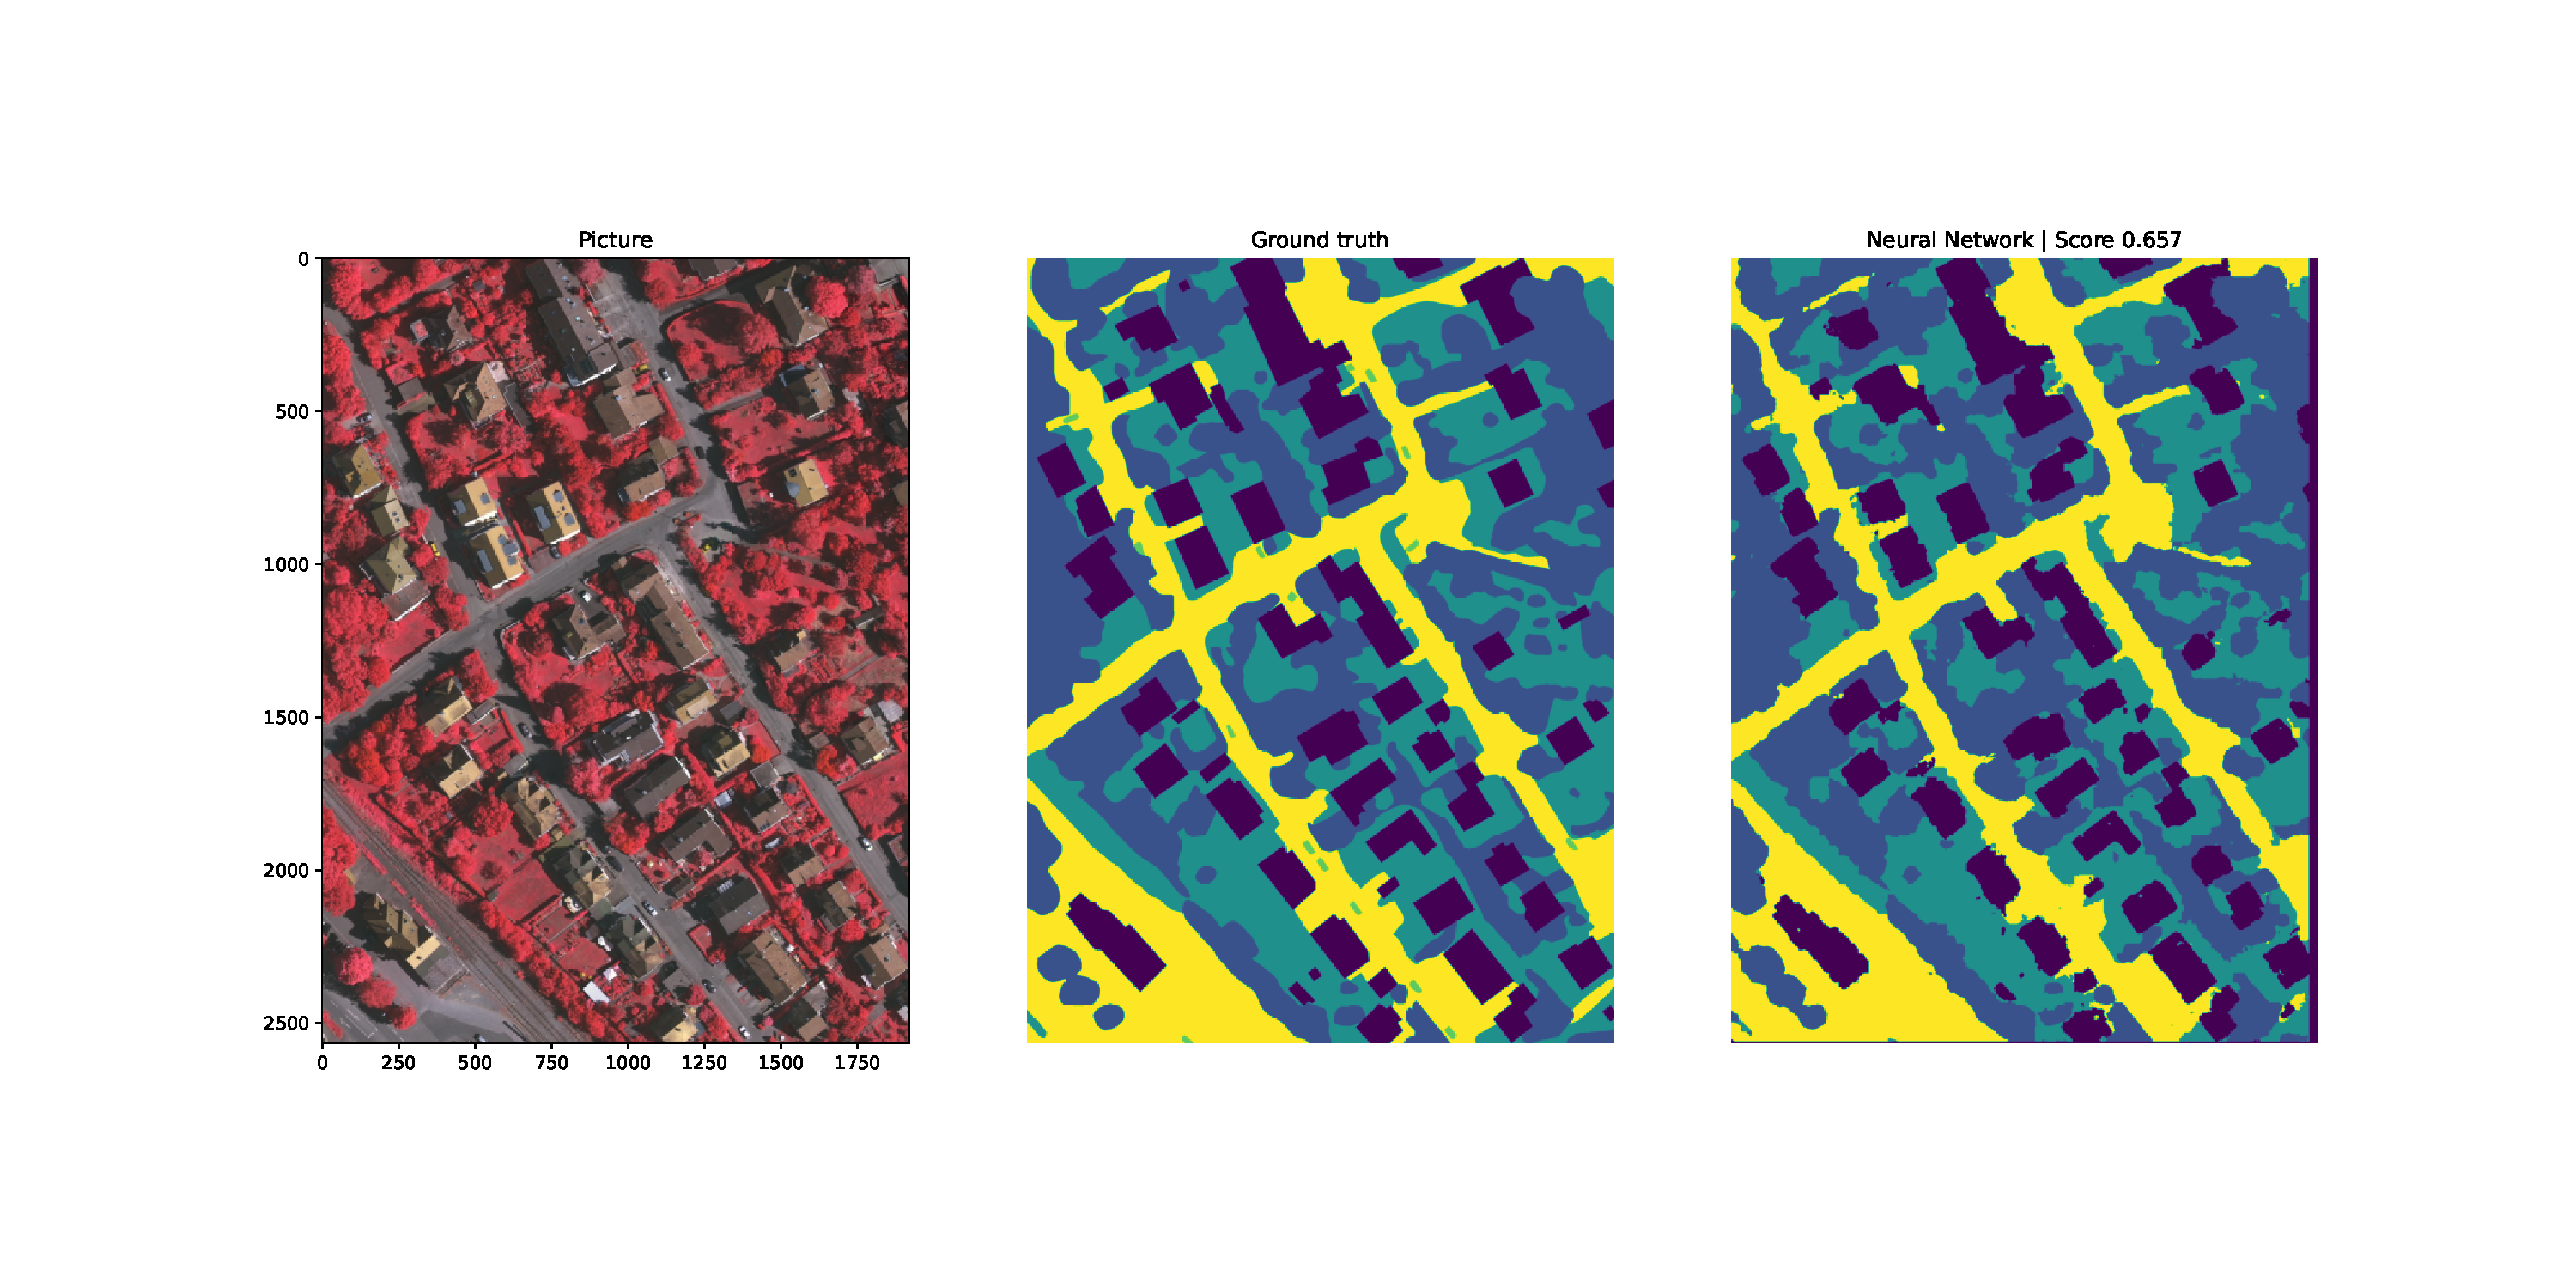
\includegraphics[width=\textwidth]{images/Patch64_scratch_train.pdf}
      \caption{Train results}
      \label{fig:q2b_train}
  \end{subfigure}
  \hspace{0.05\textwidth}
  \begin{subfigure}[b]{0.45\textwidth}
    \centering
    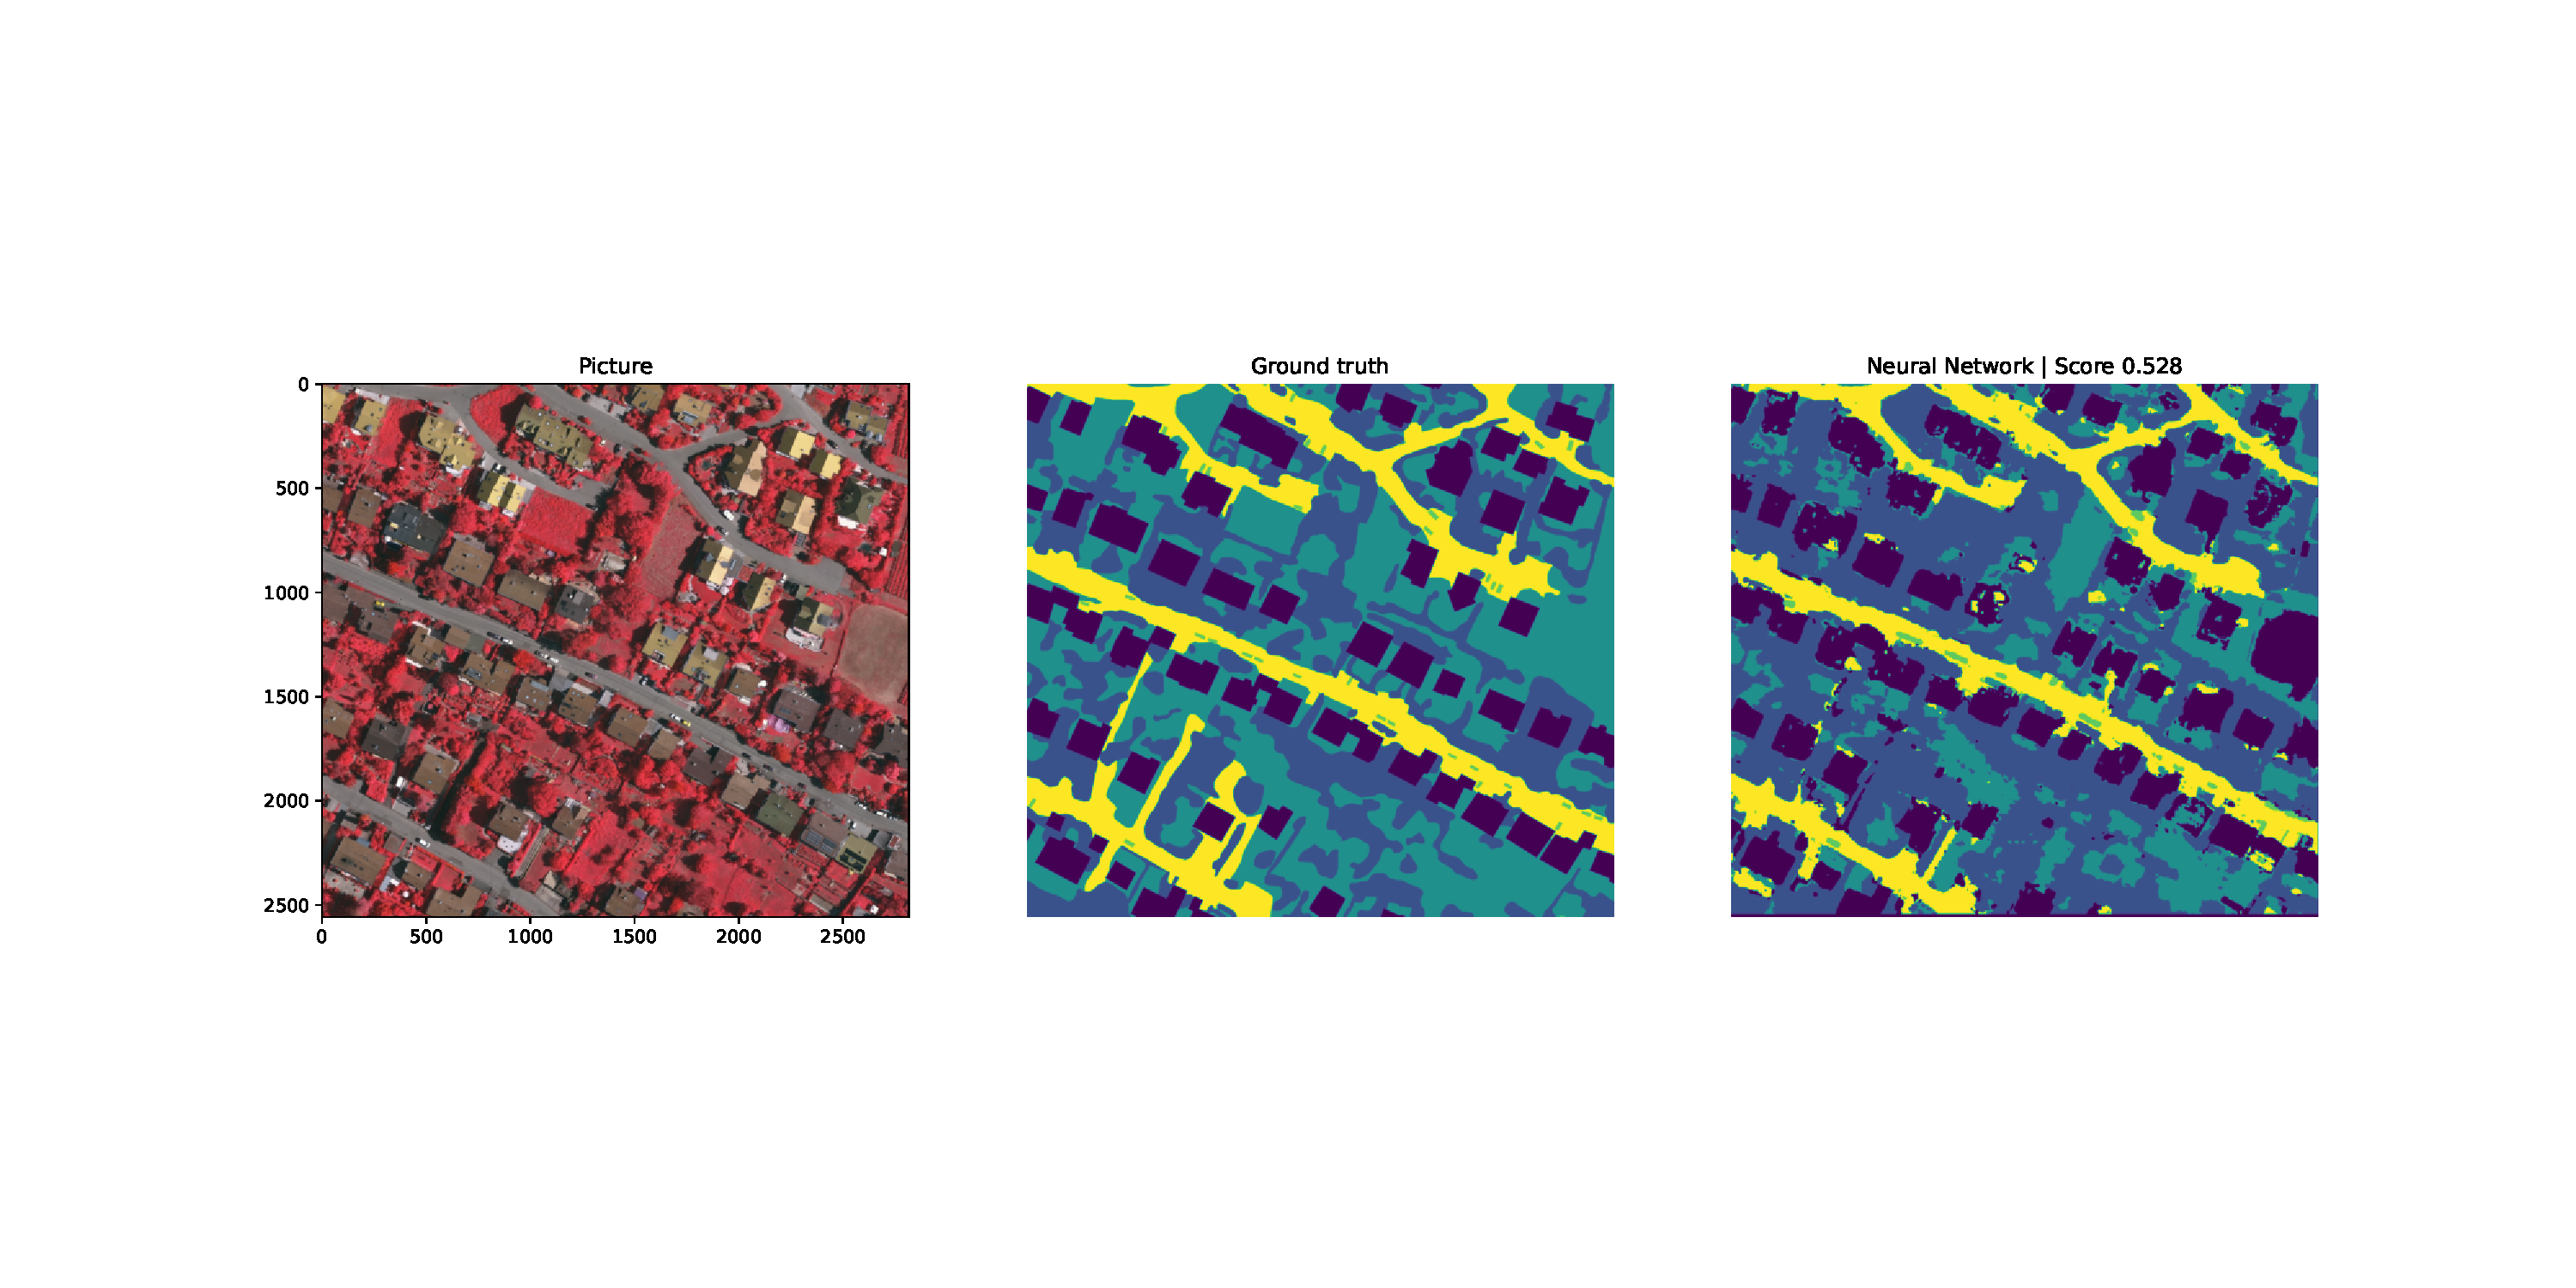
\includegraphics[width=\textwidth]{images/Patch64_scratch_test.pdf}
    \caption{test results}
    \label{fig:q2b_test}
  \end{subfigure}
  \caption{Results of predictions for item \ref{item:2b}}
  \label{fig:q2b_results}
\end{figure}

\newpage
\subsection{Item \ref{item:2c}}

Figures \ref{fig:q2c_metrics} and \ref{fig:q2c_results} show the convergency of the 20 epochs and test results obtained by using the random weights as initialization 
and dividing the train image into 128 x 128 patches with a stride of 16 pixels. Once again, slightly worse results are obtained when compared to case \ref{item:1c}.

\begin{figure}[htpb]
  \centering
  \begin{subfigure}[b]{0.32\textwidth}
      \centering
      
\includegraphics[width=\textwidth]{images/Patch128_scratch_loss.pdf}
      \caption{Loss evolution}
      \label{fig:q2c_loss}
  \end{subfigure}
  \hfill
  \begin{subfigure}[b]{0.32\textwidth}
    \centering
    
\includegraphics[width=\textwidth]{images/Patch128_scratch_score.pdf}
    \caption{Score evolution}
    \label{fig:q2c_score}
  \end{subfigure}
  \hfill
  \begin{subfigure}[b]{0.32\textwidth}
      \centering
      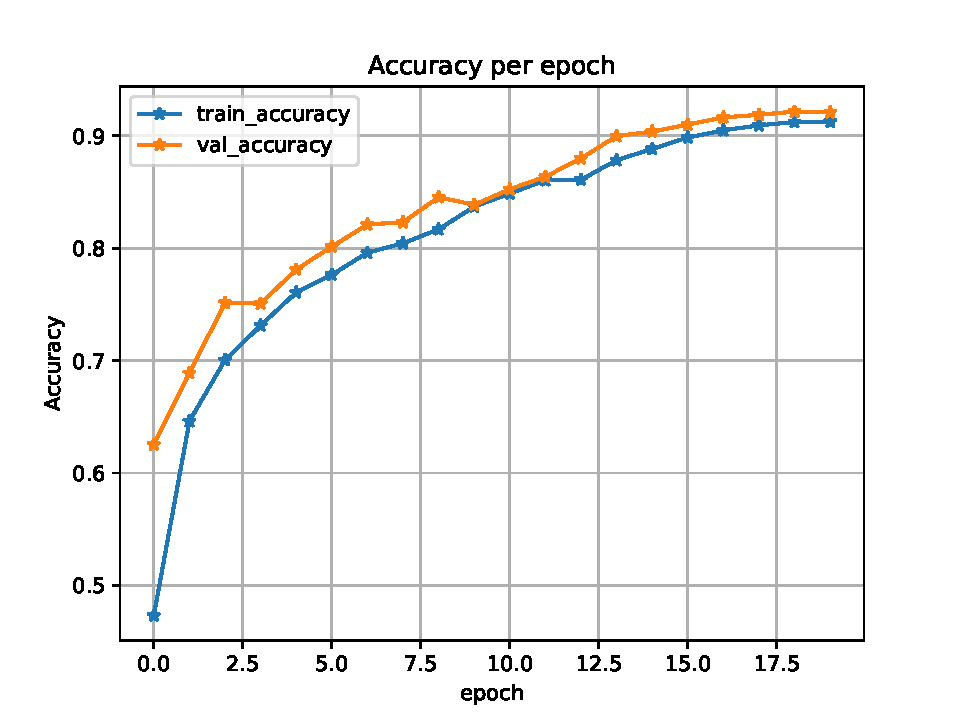
\includegraphics[width=\textwidth]{images/Patch128_scratch_acc.pdf}
      \caption{Accuracy evolution}
      \label{fig:q2c_acc}
  \end{subfigure}
  \caption{Metrics evolution during training for item \ref{item:2c}}
  \label{fig:q2c_metrics}
\end{figure}

\begin{figure}[htpb]
  \centering
  \begin{subfigure}[b]{0.45\textwidth}
      \centering
      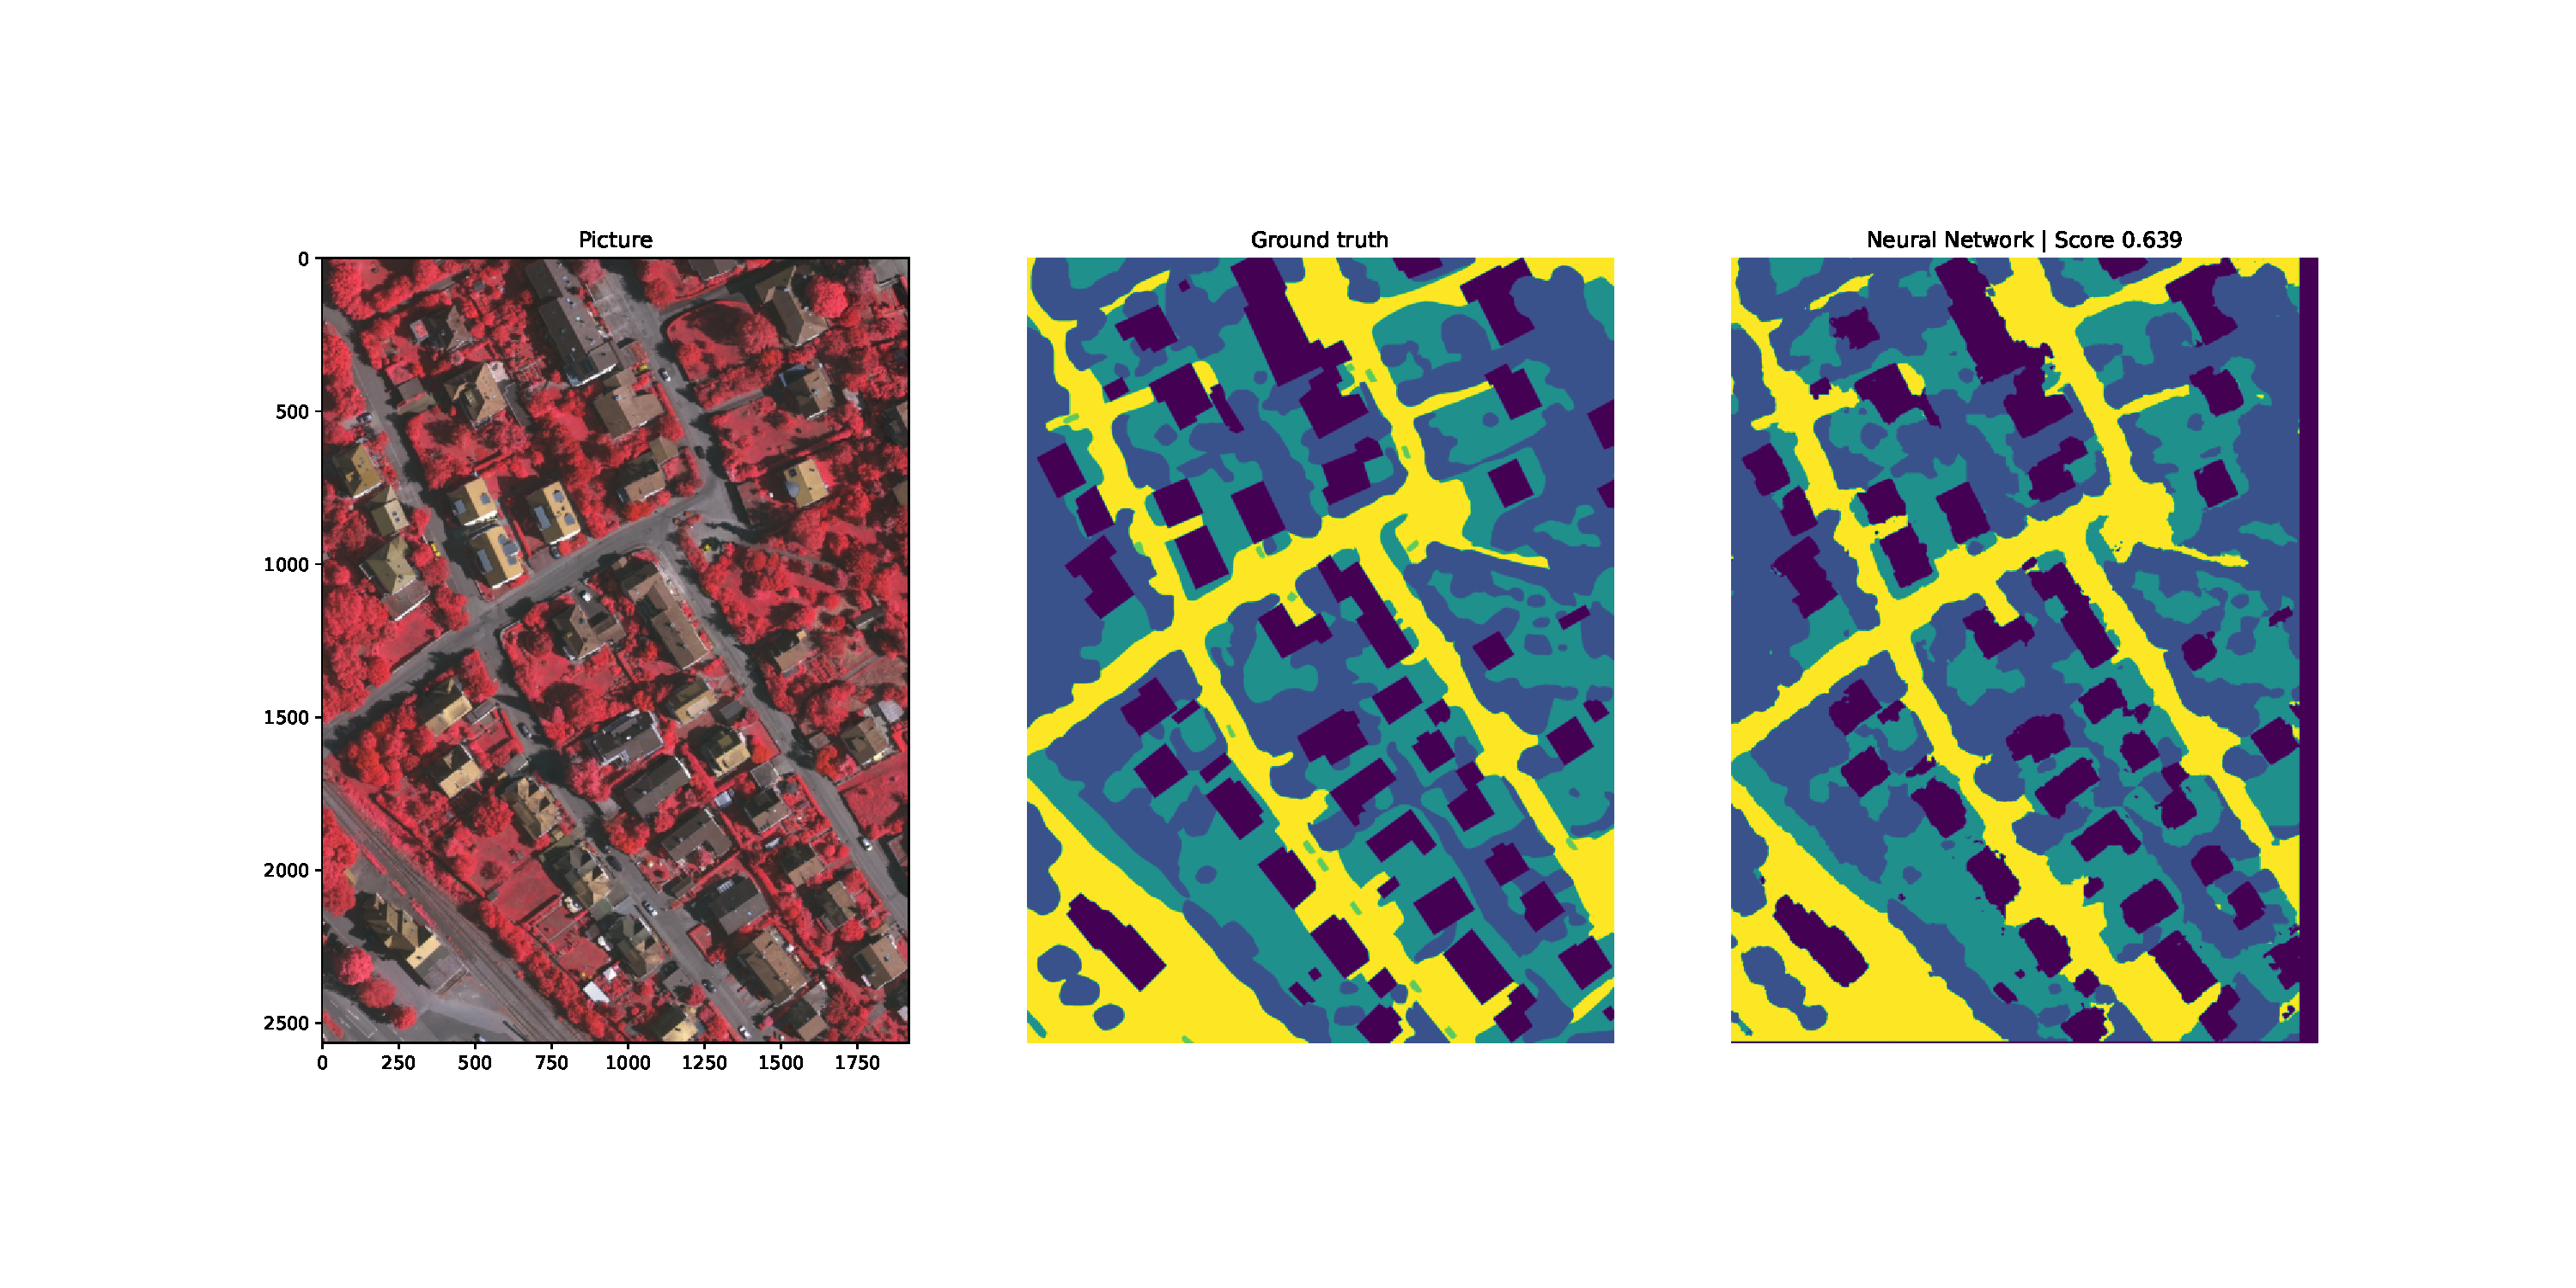
\includegraphics[width=\textwidth]{images/Patch128_scratch_train.pdf}
      \caption{Train results}
      \label{fig:q2c_train}
  \end{subfigure}
  \hspace{0.05\textwidth}
  \begin{subfigure}[b]{0.45\textwidth}
    \centering
    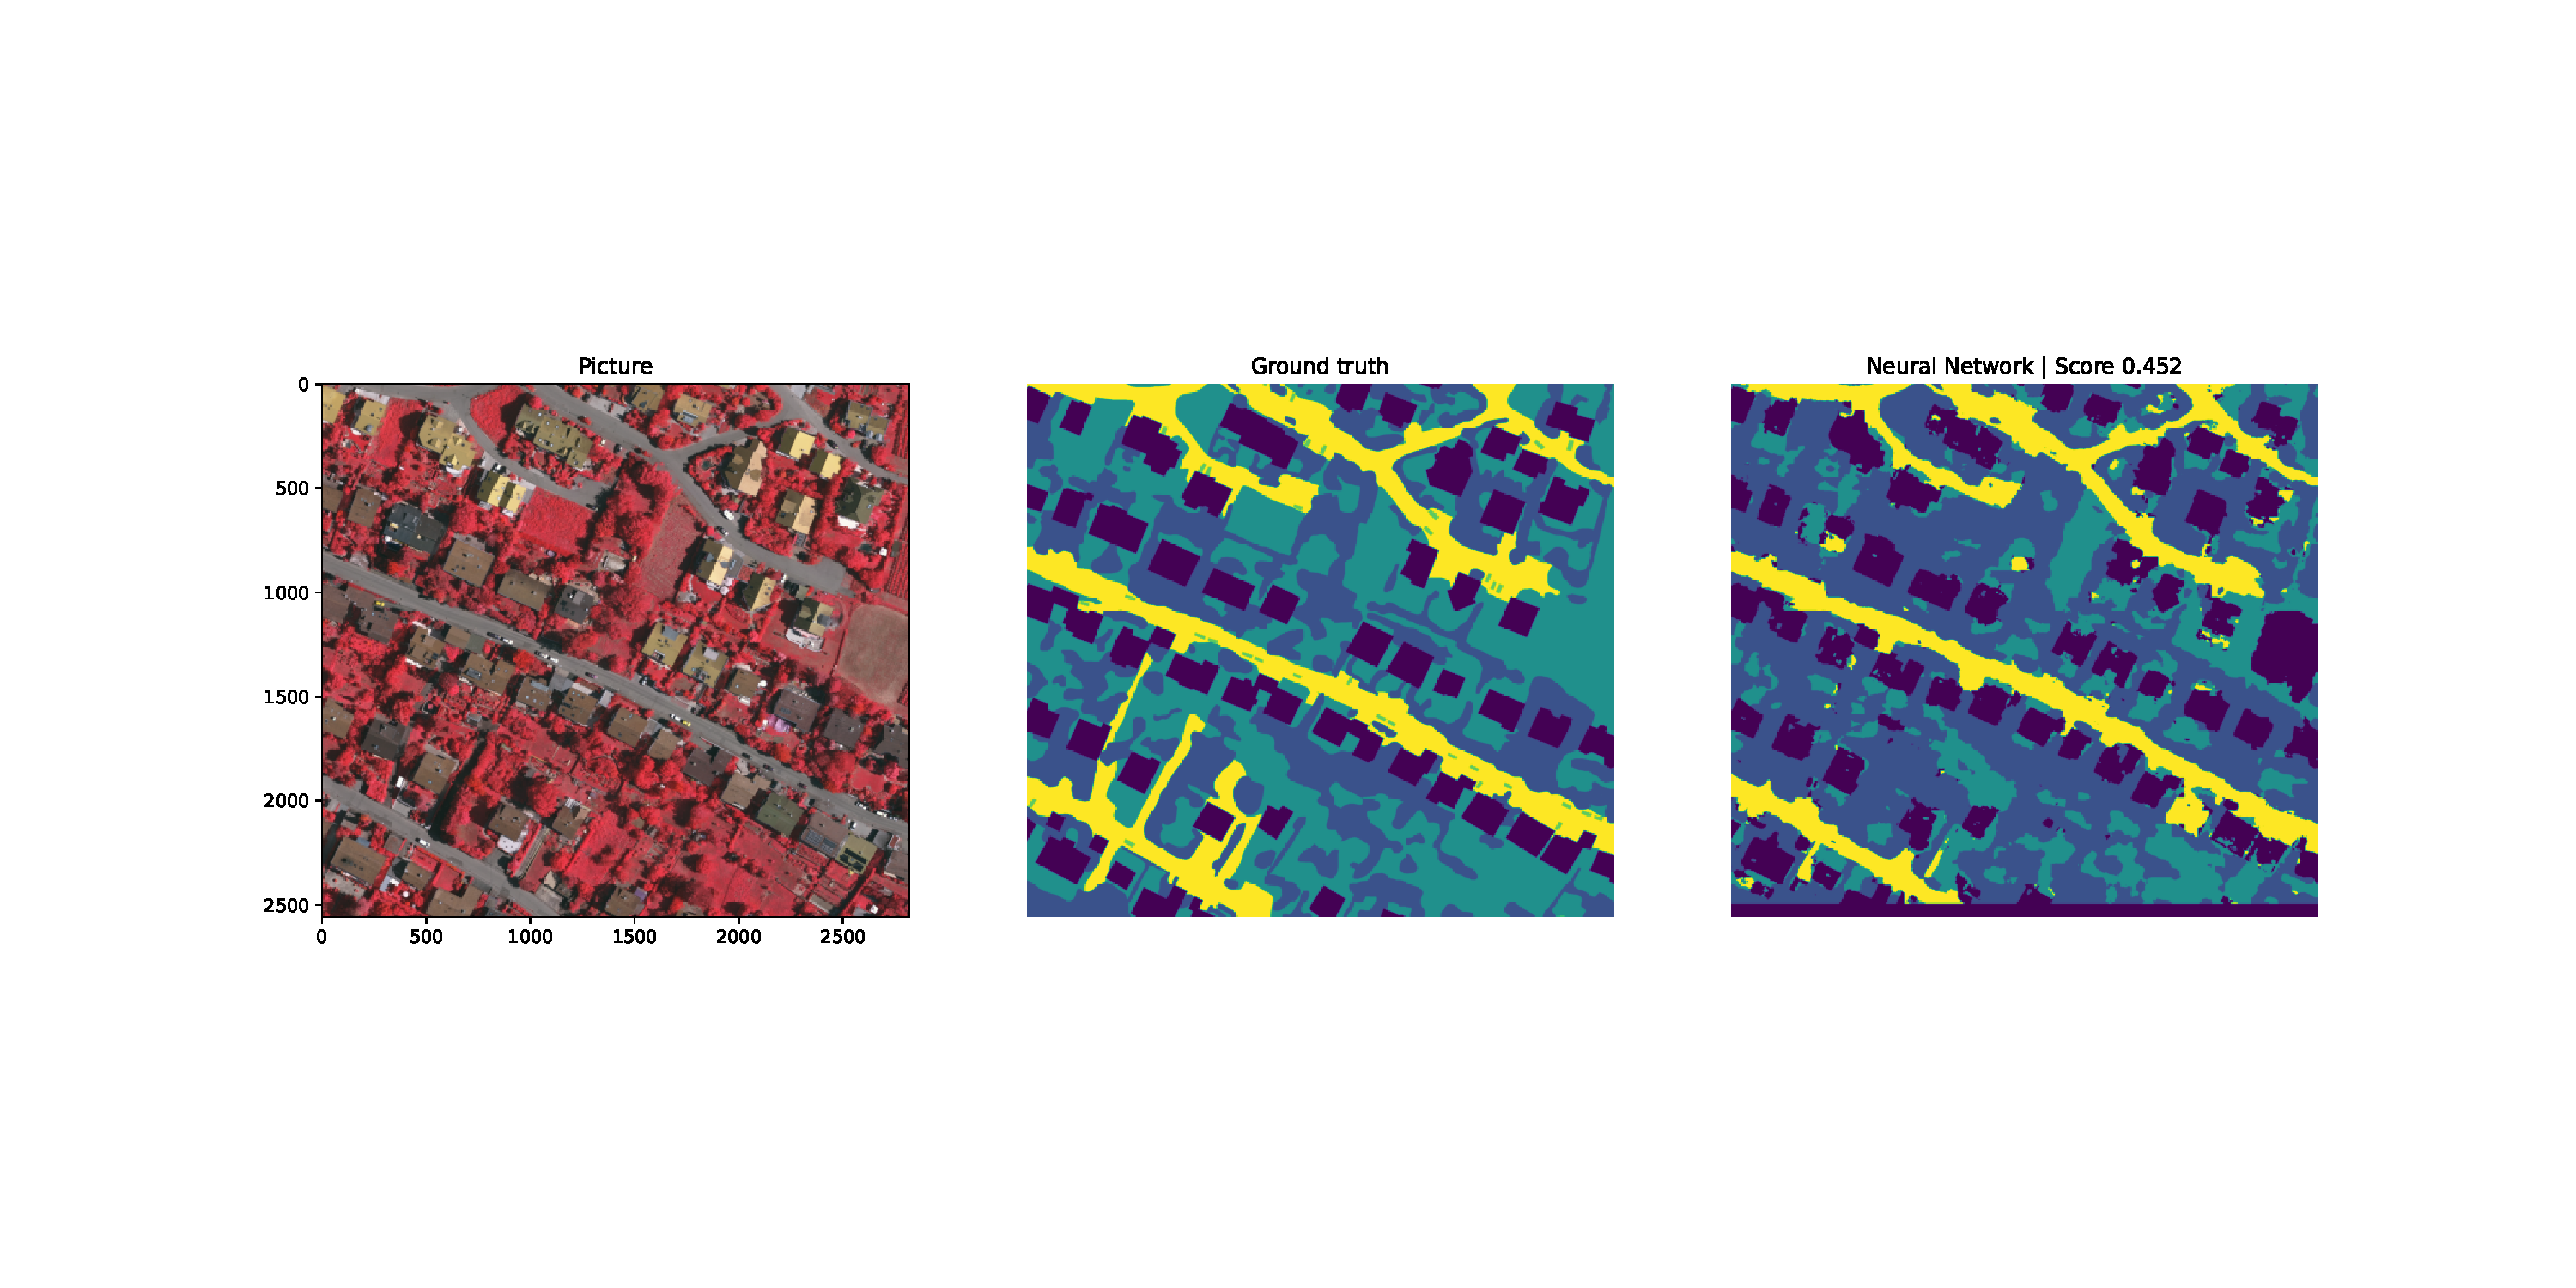
\includegraphics[width=\textwidth]{images/Patch128_scratch_test.pdf}
    \caption{test results}
    \label{fig:q2c_test}
  \end{subfigure}
  \caption{Results of predictions for item \ref{item:2c}}
  \label{fig:q2c_results}
\end{figure}

\subsection{Results Summary and Conclusions}

The patch results at the end of the training are summarized in table \ref{tab:batch_results_summ}. From this results it is possible to draw three main conclusions:
\begin{itemize}
  \item Bigger patches, such as 128 x 128 tend to present better values than smaller patches. This is probably due to the greater information arera they provide \
    to the model when compared to their smaller, more localized, couterparts
  \item Starting from the ImageNet weights allow better performances at the end of the 20 epochs
  \item The change in initialization of the weights does not change considerably the training time for 20 epochs
\end{itemize}

\begin{table}[htpb]
  \centering
  \begin{tabular}{l|c|c|c|c|c|c|c|}
    Exp             &	train acc	      & train loss	& train IoU  & val acc & val loss	 & val IoU & training time \\
    \hline
    \ref{item:1a}   & 79.0\%          & 0.472       & 0.648      & 79.6\%  & 0.486     & 0.644   & 18.20 min     \\
    \ref{item:1b}   & 86.8\%          & 0.281       & 0.744      & 87.8\%  & 0.257     & 0.754   & 20.03 min     \\
    \ref{item:1c}   & 96.8\%          & 0.063       & 0.890      & 97.0\%  & 0.059     & 0.900   & 30.69 min     \\
    \ref{item:2a}   & 75.4\%          & 0.561       & 0.602      & 76.5\%  & 0.578     & 0.604   & 19.11 min     \\
    \ref{item:2b}   & 82.0\%          & 0.398       & 0.672      & 83.3\%  & 0.366     & 0.685   & 21.00 min     \\
    \ref{item:2c}   & 91.2\%          & 0.177       & 0.788      & 92.1\%  & 0.157     & 0.798   & 29.82 min     \\
    \hline
  \end{tabular}
  \caption{Results summary for batch training}
  \label{tab:batch_results_summ}
\end{table}

The same conclusions can be achieved by analizing the results summary for the whole train and test images regarding precision, recall and F1 score. It should be
kept in mind that this scores were calculated using the {\tt scikit-learn} functions having the average by classes taken using the {\tt average='weighted'} option.
It is also important to notice that, while the train and validation differences at the end of the training are very small, the differences in performance between
the train and test images are not neglegible.

\begin{table}[htpb]
  \centering
  \begin{tabular}{l|c|c|c|c|c|c|}
    Exp             &	train precision	& train recall	& train F1 score  &	test precision  & test recall	& test F1 score \\
    \hline
    \ref{item:1a}   & 82.31\%         & 81.91\%       & 81.87\%         & 75.32\%         & 72.28\%     & 71.07\%       \\
    \ref{item:1b}   & 90.58\%         & 90.28\%       & 90.32\%         & 76.95\%         & 75.00\%     & 74.30\%       \\
    \ref{item:1c}   & 97.51\%         & 97.42\%       & 97.44\%         & 78.34\%         & 77.08\%     & 76.73\%       \\
    \ref{item:2a}   & 78.19\%         & 77.75\%       & 77.70\%         & 72.68\%         & 69.50\%     & 68.36\%       \\
    \ref{item:2b}   & 85.36\%         & 84.87\%       & 84.89\%         & 74.66\%         & 71.62\%     & 70.12\%       \\
    \ref{item:2c}   & 93.93\%         & 93.77\%       & 93.79\%         & 75.25\%         & 73.11\%     & 71.92\%       \\
    \hline
  \end{tabular}
  \caption{Results summary for train and test image}
  \label{tab:img_results_summ}
\end{table}

Figures \ref{fig:q1_cm_results} and \ref{fig:q2_cm_results} represent the prediction results for train and test images in terms of confusion matrices, with each 
class being normalized by its real labels. It is interesting to notice that the greatest source of confusion between predictions lays between classes 1 (Tree) and 
2 (Low vegetation), that are similar in color and aspect when observed in the images. Once again, it is made evident that the performance in the train image is 
far superior from the one in the test image.

\begin{figure}[htpb]
  \centering
  \begin{subfigure}[b]{0.47\textwidth}
      \centering
      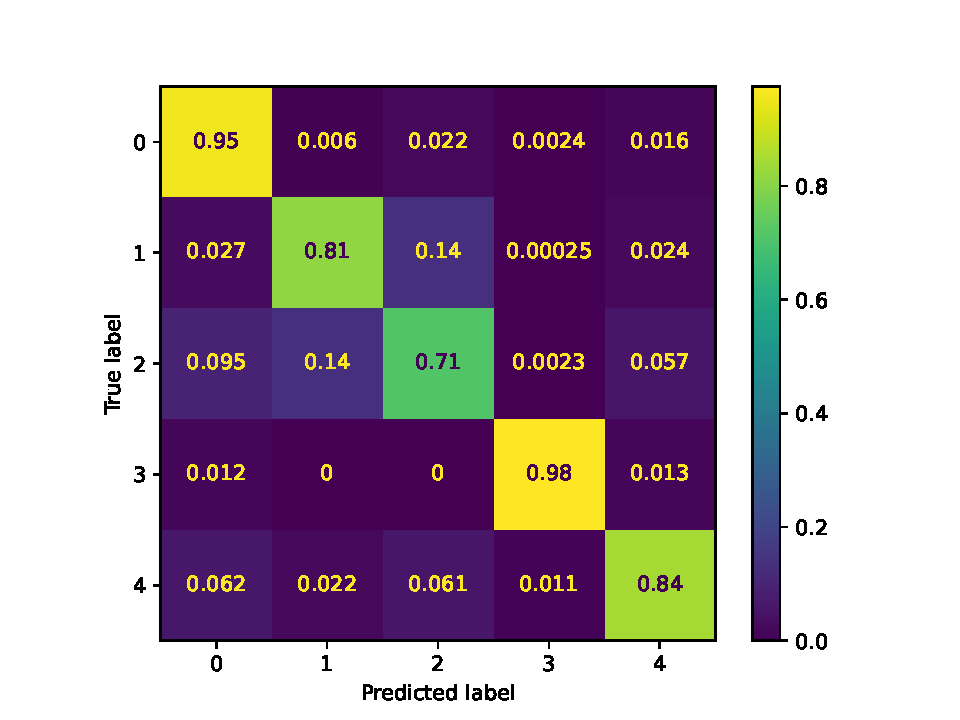
\includegraphics[width=\textwidth]{images/Patch32_imagenet_cm_train.pdf}
      \caption{Item \ref{item:1a} train results}
      \label{fig:q1a_cm_train}
  \end{subfigure}
  \hfill
  \begin{subfigure}[b]{0.47\textwidth}
    \centering
    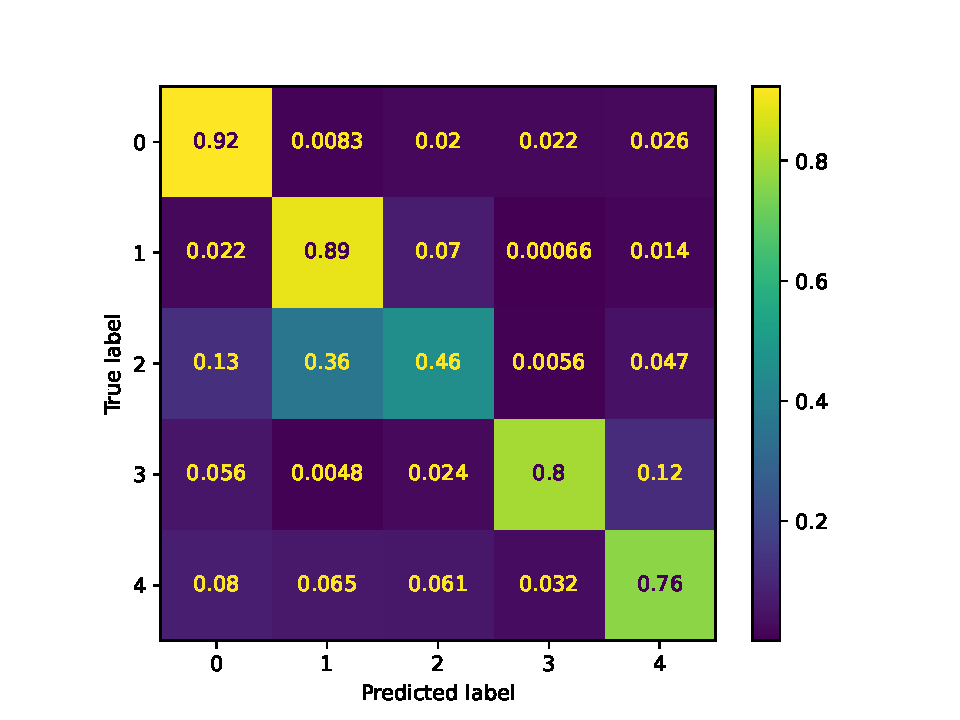
\includegraphics[width=\textwidth]{images/Patch32_imagenet_cm_test.pdf}
    \caption{Item \ref{item:1a} test results}
    \label{fig:q1a_cm_test}
  \end{subfigure}
  \hfill
  \begin{subfigure}[b]{0.47\textwidth}
    \centering
    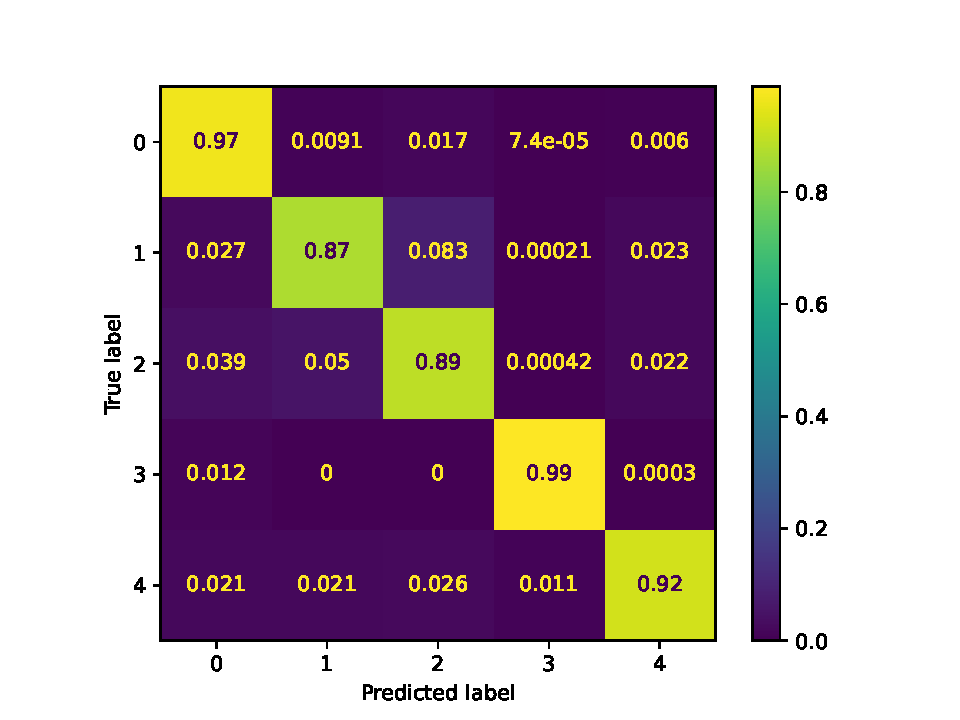
\includegraphics[width=\textwidth]{images/Patch64_imagenet_cm_train.pdf}
    \caption{Item \ref{item:1b} train results}
    \label{fig:q1b_cm_train}
  \end{subfigure}
  \hfill
  \begin{subfigure}[b]{0.47\textwidth}
    \centering
    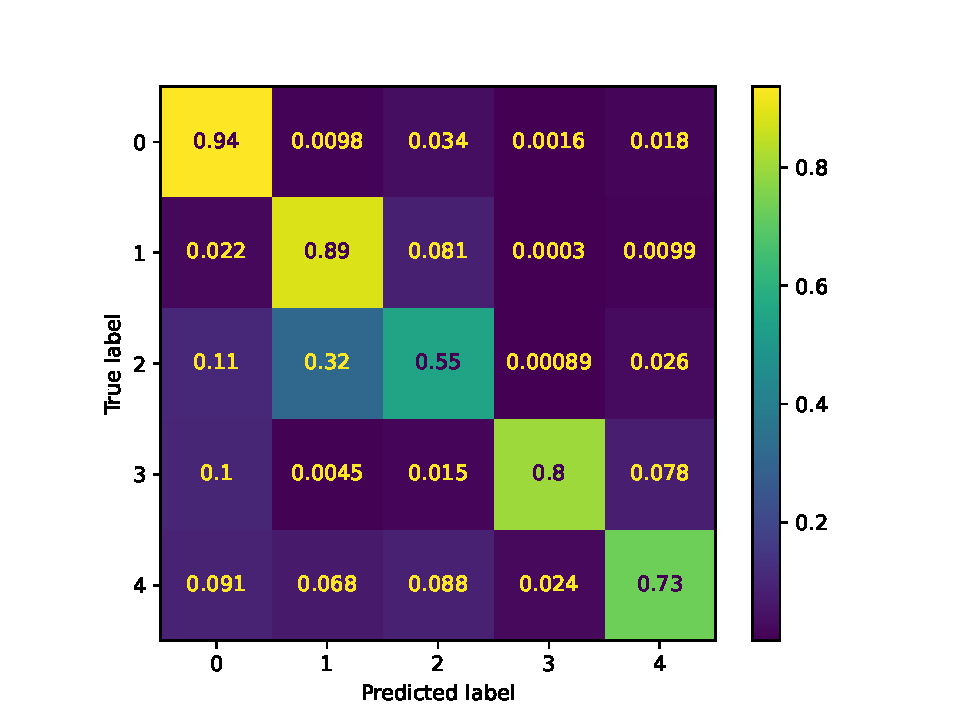
\includegraphics[width=\textwidth]{images/Patch64_imagenet_cm_test.pdf}
    \caption{Item \ref{item:1b} test results}
    \label{fig:q1b_cm_test}
  \end{subfigure}
  \hfill
  \begin{subfigure}[b]{0.47\textwidth}
    \centering
    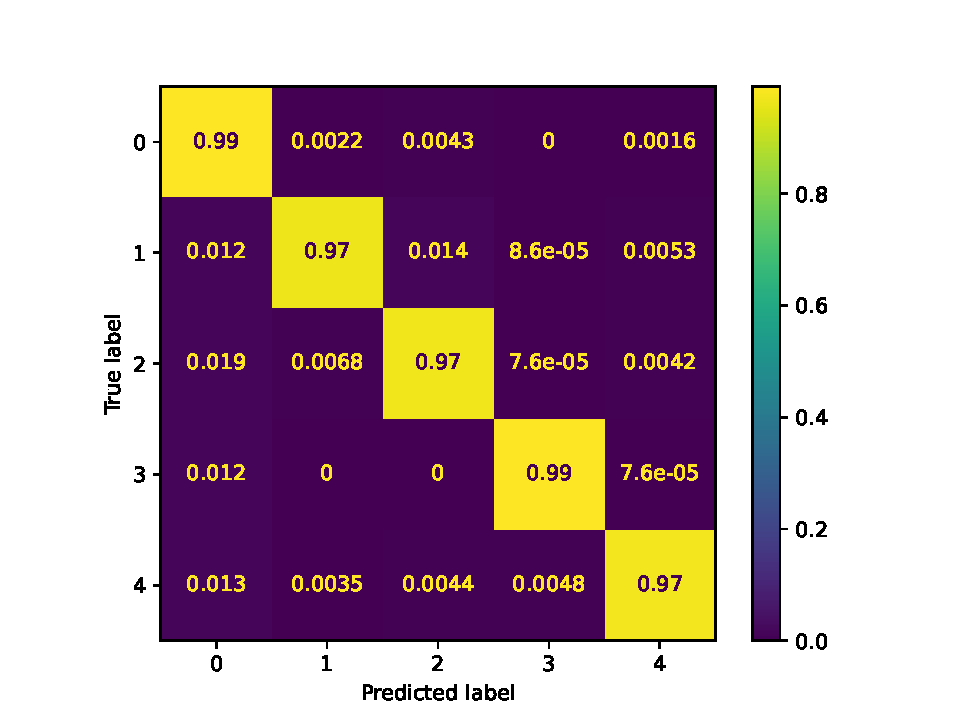
\includegraphics[width=\textwidth]{images/Patch128_imagenet_cm_train.pdf}
    \caption{Item \ref{item:1c} train results}
    \label{fig:q1c_cm_train}
  \end{subfigure}
  \hfill
  \begin{subfigure}[b]{0.47\textwidth}
    \centering
    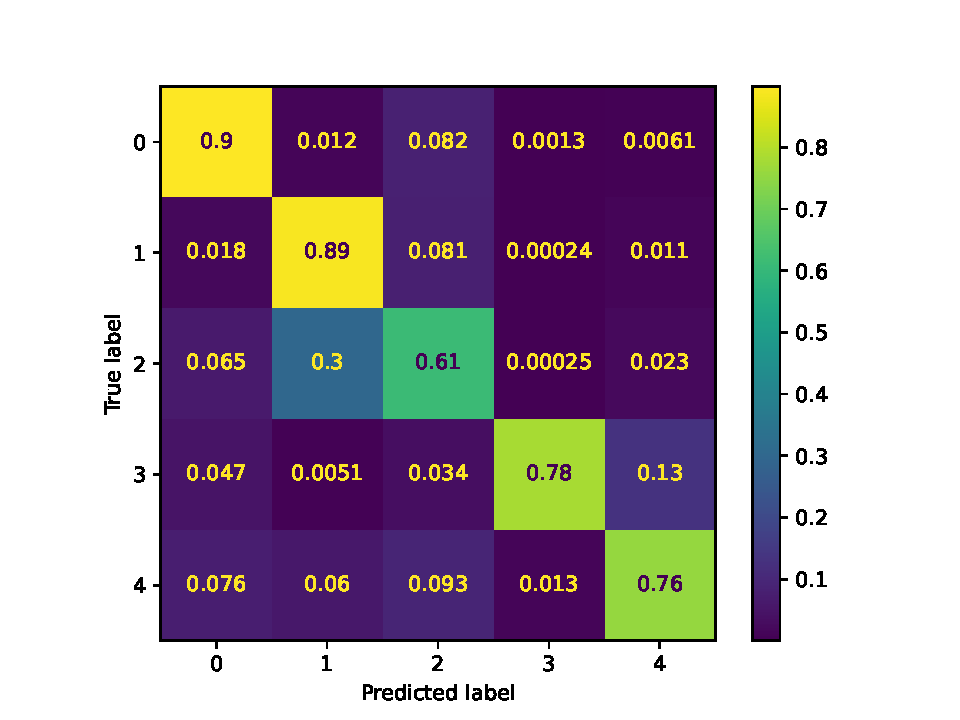
\includegraphics[width=\textwidth]{images/Patch128_imagenet_cm_test.pdf}
    \caption{Item \ref{item:1c} test results}
    \label{fig:q1c_cm_test}
  \end{subfigure}
  \hfill
  \caption{Confusion matrices for performed tests item \ref{item:1}}
  \label{fig:q1_cm_results}
\end{figure}

\begin{figure}[htpb]
  \centering
  \begin{subfigure}[b]{0.47\textwidth}
    \centering
    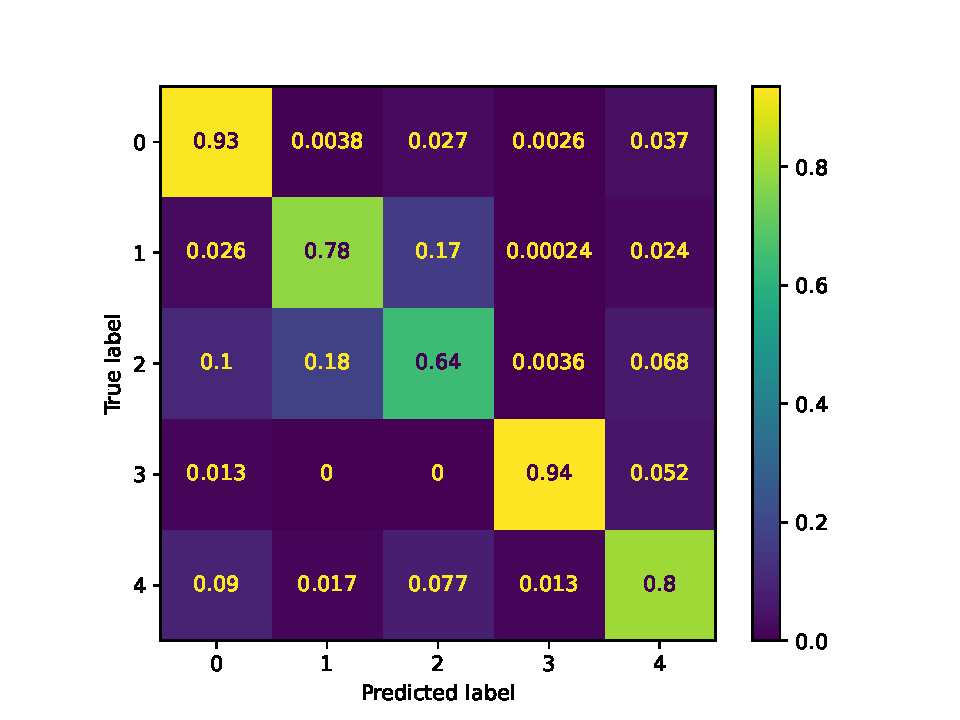
\includegraphics[width=\textwidth]{images/Patch32_scratch_cm_train.pdf}
    \caption{Item \ref{item:2a} train results}
    \label{fig:q2a_cm_train}
  \end{subfigure}
  \hfill
  \begin{subfigure}[b]{0.47\textwidth}
    \centering
    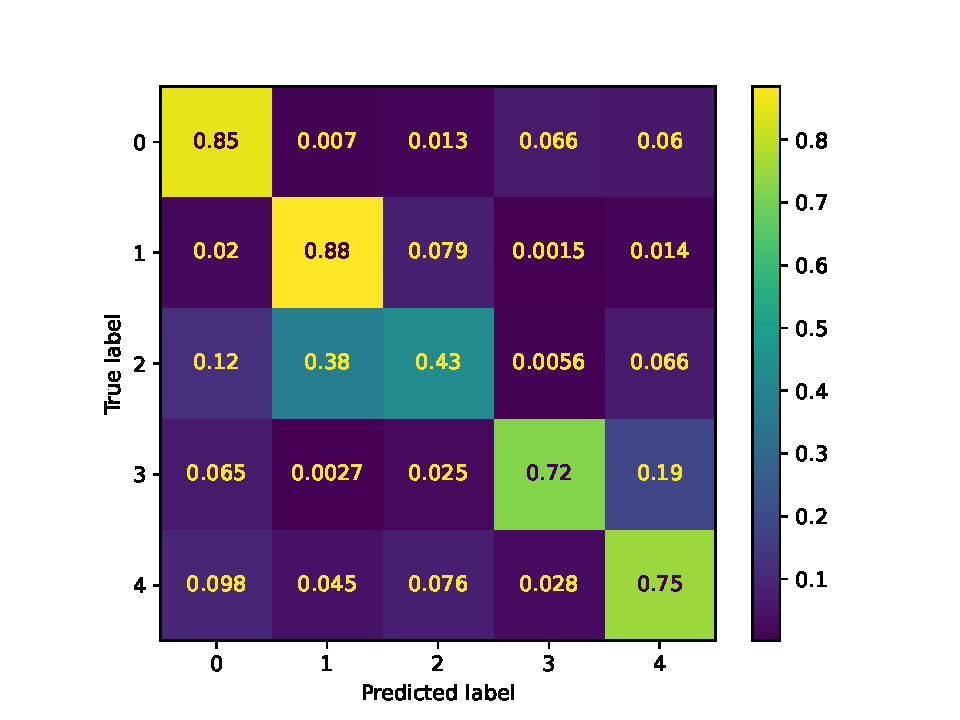
\includegraphics[width=\textwidth]{images/Patch32_scratch_cm_test.pdf}
    \caption{Item \ref{item:2a} test results}
    \label{fig:q2a_cm_test}
  \end{subfigure}
  \hfill
  \begin{subfigure}[b]{0.47\textwidth}
    \centering
    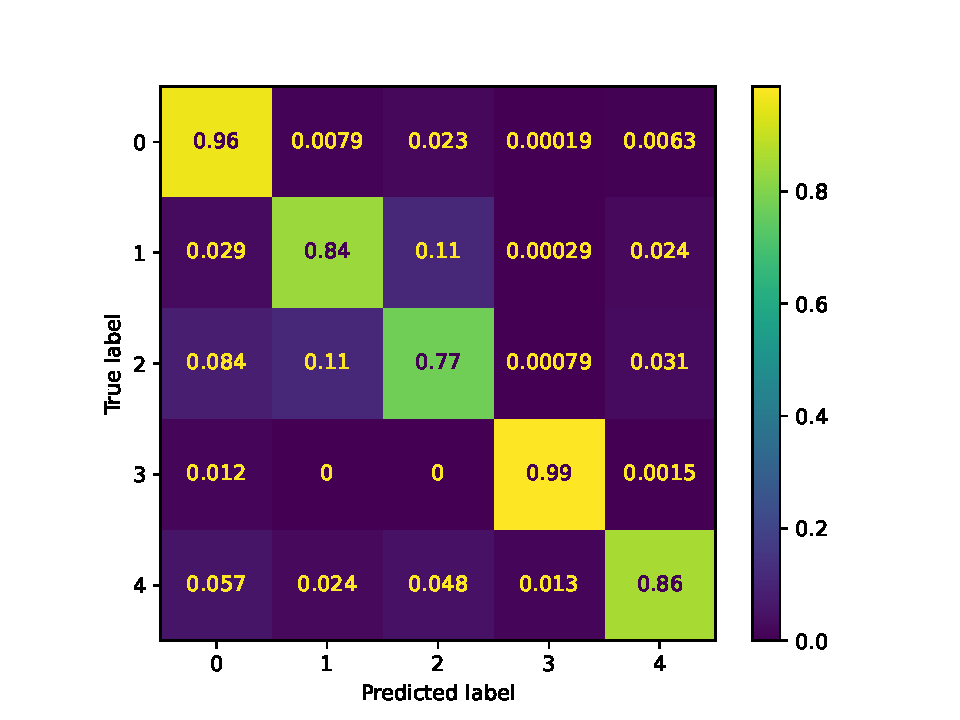
\includegraphics[width=\textwidth]{images/Patch64_scratch_cm_train.pdf}
    \caption{Item \ref{item:2b} train results}
    \label{fig:q2b_cm_train}
  \end{subfigure}
  \hfill
  \begin{subfigure}[b]{0.47\textwidth}
    \centering
    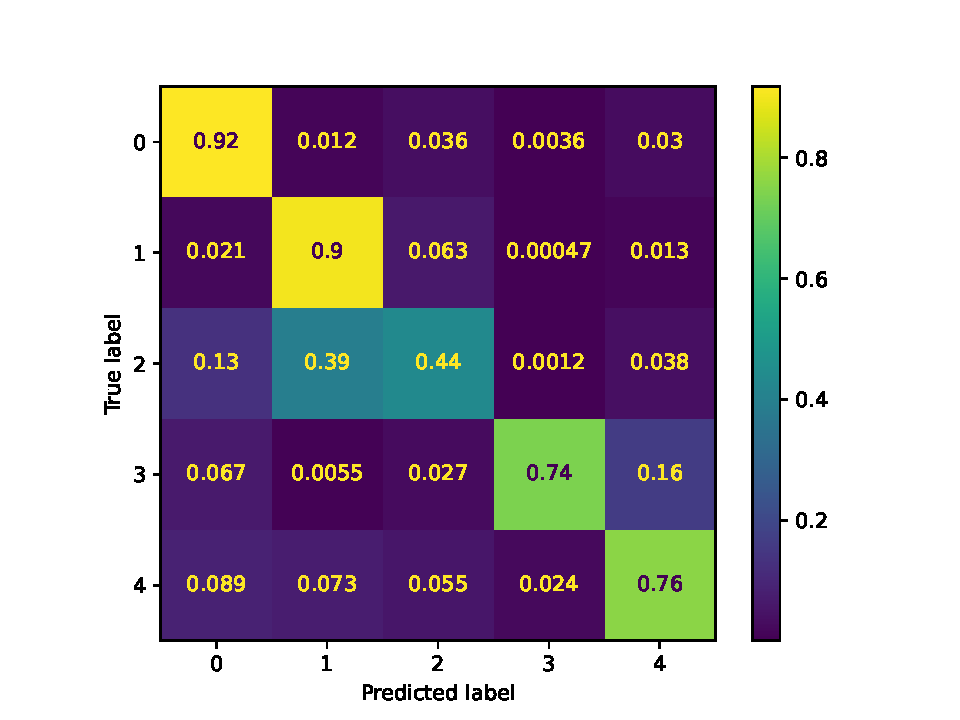
\includegraphics[width=\textwidth]{images/Patch64_scratch_cm_test.pdf}
    \caption{Item \ref{item:2b} test results}
    \label{fig:q2b_cm_test}
  \end{subfigure}
  \hfill
  \begin{subfigure}[b]{0.47\textwidth}
    \centering
    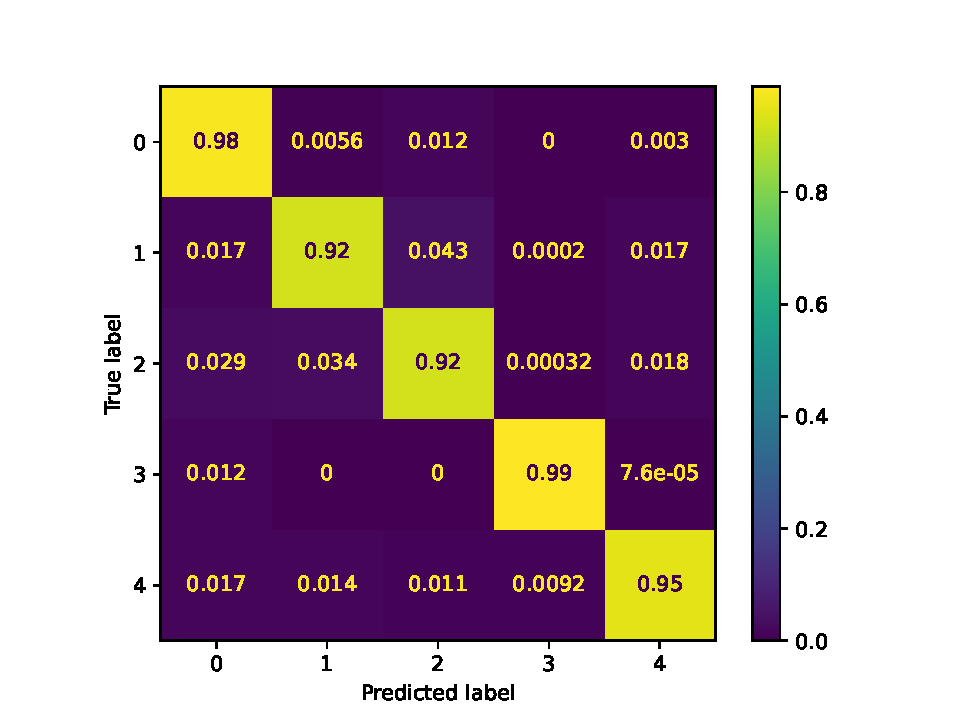
\includegraphics[width=\textwidth]{images/Patch128_scratch_cm_train.pdf}
    \caption{Item \ref{item:2c} train results}
    \label{fig:q2c_cm_train}
  \end{subfigure}
  \hfill
  \begin{subfigure}[b]{0.47\textwidth}
    \centering
    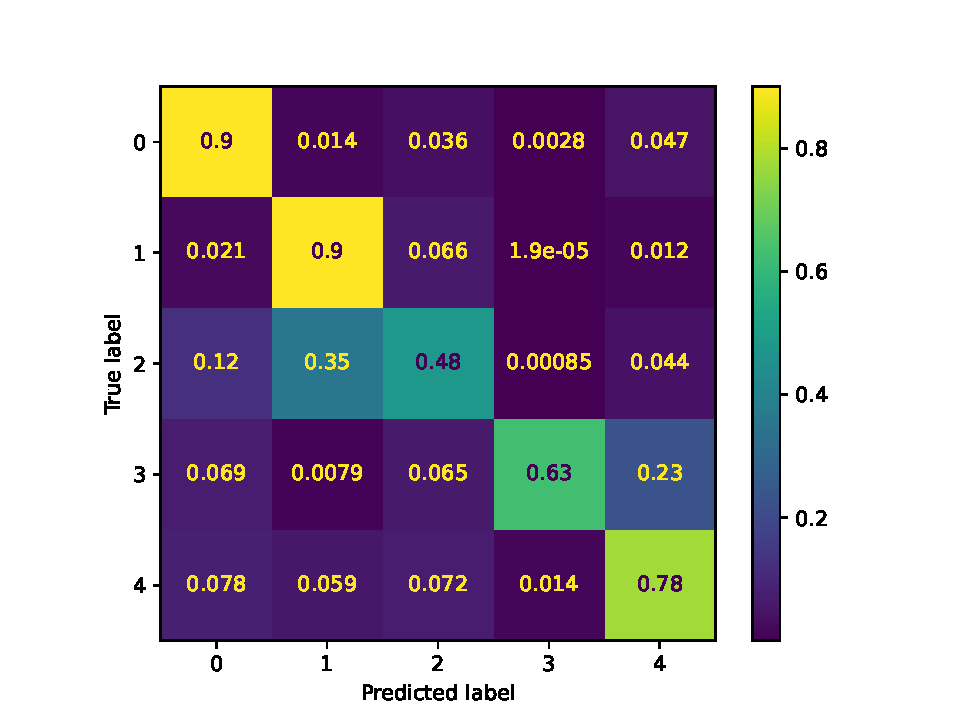
\includegraphics[width=\textwidth]{images/Patch128_scratch_cm_test.pdf}
    \caption{Item \ref{item:2c} test results}
    \label{fig:q2c_cm_test}
  \end{subfigure}
  \hfill
  \caption{Confusion matrices for performed tests item \ref{item:2}}
  \label{fig:q2_cm_results}
\end{figure}






%%%%%%%%%%%%%%%%%%%%%%%%%%%%%%%%%%%%%%%%%%%%%%%%%%%

\bibliographystyle{apalike}
\bibliography{export}

\end{document}